%%% Time-stamp: <2023-06-14 11:53:28 vladimir>
%%% Copyright (C) 2019-2023 Vladimir G. Ivanović
%%% Author: Vladimir G. Ivanović <vladimir@acm.org>
%%% ORCID: https://orcid.org/0000-0002-7802-7970
% arara: lualatex

%%% Time-stamp: <2023-07-11 15:05:00 vladimir>
%%% Copyright (C) 2019-2023 Vladimir G. Ivanović
%%% Author: Vladimir G. Ivanović <vladimir@acm.org>
%%% ORCID: https://orcid.org/0000-0002-7802-7970

% !TEX TS-program = lualatex

\DocumentMetadata{pdfversion=2.0}
\nonstopmode\synctex=1
%\RequirePackage[l2tabu, orthodox]{nag}

\documentclass[letterpaper,twoside,openright,article,12pt]{memoir} % SJSU EDD Guidelines Checklist #18

\tracinglostcharacters=3

\usepackage[pagewise]{lineno}
\usepackage{adforn}
\usepackage{array}
\usepackage{authblk}
\usepackage{booktabs}
\usepackage{calc}
\usepackage[labelfont=rm]{caption}
\usepackage{csquotes}
\usepackage{datetime2}
\usepackage[shortlabels]{enumitem}
% \usepackage[draft,inline,margin=false]{fixme}
\usepackage{fontspec}
\usepackage[ragged]{footmisc}
\usepackage[edges]{forest}
\usepackage[left=1.5in, top=1.25in, bottom=1.25in, nomarginpar]{geometry}
\usepackage{graphicx}
\usepackage{imakeidx}
\usepackage{makecell}
\usepackage{multirow}
\usepackage{mVersion}
\usepackage{orcidlink}
\usepackage{pgfplots}
%\pgfplotsset{compat/show suggested version=false}
% \usepackage{subcaption}
\usepackage{prettyref}
\newrefformat{figp}{Figure \ref{#1},   \textit{\titleref{#1}} on p.\pageref{#1}}
\newrefformat{ch}{Chapter \ref{#1},    \textit{\titleref{#1}}}
\newrefformat{sec}{Section \ref{#1},   \textit{\titleref{#1}}}
\newrefformat{tab}{Table \ref{#1},     \textit{\titleref{#1}}}
\newrefformat{fig}{Figure \ref{#1},    \textit{\titleref{#1}}}
\newrefformat{appx}{Appendix \ref{#1}, \textit{\titleref{#1}}}
\usepackage[normalem]{ulem}
\usepackage{tikz}
% \usetikzlibrary{graphdrawing.trees}
% \tikzstyle{every node}=[draw=black,thick,rectangle]
\usepackage{url}
%\usepackage[nospace]{varioref}
\usepackage{xcolor}
\usepackage{hyperref}           % Should be last

\usepackage{polyglossia}
\setdefaultlanguage{american}
\usepackage[style=apa,sortcites=false,sorting=nyt,backend=biber]{biblatex}
\DeclareLanguageMapping{american}{american-apa}

% \setVersion{1.0}                % Major.minor.build; Increment major and minor as appropriate
\increaseBuild{}

\setmainfont[Ligatures=TeX,Numbers=OldStyle]{Alegreya}
\setsansfont[Ligatures=TeX,Numbers=OldStyle]{Alegreya Sans}
\setmonofont[Scale=MatchLowercase]{Fira Mono}
\setmathtt[Scale=MatchLowercase]{Fira Math}

\pagestyle{plain}               % SJSU EDD Guidelines Checklist #10
%\checkthelayout

\raggedright%                    % SJSU EDD Guidelines Checklist #2, #4

% % See memman.pdf p.52
% % \clubpenalty=10000
% % \widowpenalty=10000
% \sloppybottom%

\setlength{\footskip}{\onelineskip}
\setlength{\footnotesep}{\onelineskip}

\def\UrlFont{\footnotesize\texttt}
\urlstyle{tt}

\pgfplotsset{compat=default}

\setlength{\parindent}{0.25in}  % SJSU EDD Guidelines Checklist #3

\DoubleSpacing%

\tightlists%
\setlist[1]{labelindent=\parindent}
\setlist[itemize]{leftmargin=*}
\setlist[enumerate]{leftmargin=*}
\setlist[description]{leftmargin=2\parindent}

\setsecnumdepth{subsubsection}
\maxsecnumdepth{subsubsection}
\settocdepth{subsubsection}

% % \citeauthor prints only the last name. This command prints the author(s) first and last name.
% \newrobustcmd*{\citefirstlastauthor}{\AtNextCite{\DeclareNameAlias{labelname}{given-family}}\citeauthor}

\makechapterstyle{sjsu}{%
  \chapterstyle{article}
  \setlength{\afterchapskip}{0in}
  \renewcommand{\chapnamefont}{\normalfont\bfseries}
  \renewcommand{\chapnumfont}{\normalfont\bfseries}
  \renewcommand{\chaptitlefont}{\normalfont\bfseries}
  \renewcommand{\printchaptername}{}
  \renewcommand{\printchapternum}{}
  \renewcommand{\printchaptertitle}[1]{%          % APA Level 1 Heading: centered, bold, title case
    \SingleSpacing\centering\normalfont\bfseries\chaptitlefont{}##1}
}
\chapterstyle{sjsu}

\makechapterstyle{appdx_sjsu}{%
  \settocdepth{subsection}
  \setlength{\afterchapskip}{0in}
  \renewcommand*{\chapterheadstart}{}
  \renewcommand*{\chaptitlefont}{}
  \renewcommand*{\printchaptername}{}
  \renewcommand*{\printchapternum}{}
  % \renewcommand*{\midchapskip}{-0.24in}
  \renewcommand*{\printchaptertitle}[1]{%
  \SingleSpacing\centering{\textbf\chaptitlefont{}##1}}}

\indentafterchapter%

\setsecheadstyle{\noindent\normalfont\bfseries\raggedright}% APA Level 2 Heading: flush left, bold, title case
\setsubsecheadstyle{\noindent\normalfont\itshape\bfseries\raggedright}% APA Level 3 Heading: flush left, bold italic, title case
\setsubsubsecheadstyle{\indent\normalfont\bfseries\raggedright}% APA Level 4 Heading: indented, bold, title case, end with '.'

\setbeforesecskip{-\onelineskip}
\setbeforesubsecskip{0pt}
\setbeforesubsubsecskip{0pt}

\setaftersecskip{0pt}
\setaftersubsecskip{0pt}
\setaftersubsubsecskip{0pt}

\renewcommand{\cftchapterfont}{\normalfont\bfseries}
\renewcommand{\cftsectionfont}{\normalfont}
\renewcommand{\cftsubsectionfont}{\normalfont}
\renewcommand{\cftsubsubsectionfont}{\normalfont}

\renewcommand{\abstractnamefont}{\normalfont\centering}

\captionsetup{singlelinecheck=false,justification=raggedright,labelfont={bf,footnotesize},labelsep=newline}

%setlength{\bibitemsep}{\onelineskip}

\indexsetup{level=\chapter,toclevel=chapter}
\makeindex

%%% Local Variables:
%%% mode: latex
%%% TeX-master: "Rocketship_Education-An_Exploratory_Public_Policy_Case_Study"
%%% End:


\addbibresource{References.bib}


\pretitle{\begin{center}\normalfont}
\title{%
  ROCKETSHIP EDUCATION:\\
  AN EXPLORATORY PUBLIC POLICY CASE STUDY
} % SJSU EDD Guidelines Checklist #17
\posttitle{\end{center}} 

\date{}

\preauthor{%\
  \begin{center}
    \normalfont%
    \bigskip\bigskip\bigskip\bigskip\bigskip
    A Dissertation Presented to\\
    The Faculty of the Connie L. Lurie College of Education\\
    San José State University\\
    \bigskip\bigskip\bigskip\bigskip\bigskip
    In Partial Fulfillment of the Requirements for the Degree\\
    Doctor of Education\\
  \end{center}
}

\author{%
  \begin{center}
    by\\
    Vladimir Gresham Ivanović \protect\orcidlink{0000–0002–7802–7970}\\\bigskip\bigskip
  \end{center}
}

\postauthor{%
  \begin{center}
    December 2023 \vfill Version \version{} created on \DTMnow
  \end{center}
}

% \forestset{%
%   direction switch/.style={%
%     for tree={edge+=thick, font=\sffamily},
%     where level>=1{folder, grow'=0}{for children=forked edge},
%     where level=2{}{draw},
%   },
% }

\hypersetup{%
  pdfinfo={%
    Title={Rocketship Education: An Exploratory Public Policy Case Study},
    Author={Vladimir Gresham Ivanović},
    Language={en-US},
    Subject={An Ed.D. dissertation that examines the finances of Rocketship Education, a charter school management organization, using a public policy lens.},
    Keywords={Rocketship Education, charter management organization, CMO, charter finances, education public policy},
    Version={\version}
  }
}

\begin{document}
%%%%%%%%%%%%%%%%%%%%%%%%%%%%%%%%%%%%%%%%%%%%%%%%%%%%%%%%%%%%%%%%%
\frontmatter{}
%%%%%%%%%%%%%%%%%%%%%%%%%%%%%%%%%%%%%%%%%%%%%%%%%%%%%%%%%%%%%%%%%

\maketitle

\thispagestyle{empty}           % for title page
\pagestyle{empty}               % for copyright, signature, & abstract pages

\newpage%%% Time-stamp: <2022-06-12 17:26:32 vladimir>
%%% Copyright (C) 2019-2022 Vladimir G. Ivanović
%%% Author: Vladimir G. Ivanović <vladimir@acm.org>
%%% ORCID: https://orcid.org/0000-0002-7802-7970

\begin{vplace}[1]
\footnotesize
    \begin{center}
        Copyright © 2022 Vladimir Gresham Ivanović.\\
        All Rights Reserved.\\\bigskip\bigskip
        \textit{Rocketship Education: An Exploratory Public Policy Case Study}\\
        by Vladimir Gresham Ivanović\\
        is licensed under a \\
        Creative Commons Attribution-NonCommercial-ShareAlike 4.0 International License\\
        which may be viewed at:\\
        \url{http://creativecommons.org/licenses/by-nc-sa/4.0/legalcode}
    \end{center}
 \end{vplace}
 
%%% Local Variables:
%%% mode: plain-tex
%%% TeX-master: "Rocketship_Education-An_Exploratory_Public_Policy_Case_Study"
%%% End:

\newpage%%% Time-stamp: <2023-07-17 15:47:07 vladimir>
%%% Copyright (C) 2019-2023 Vladimir G. Ivanović
%%% Author: Vladimir G. Ivanović <vladimir@acm.org>
%%% ORCID: https://orcid.org/0000-0002-7802-7970

\begin{vplace}[0.25]

\begin{center}
The Designated Dissertation Committee Approves the Dissertation Titled\\
\vspace{2\baselineskip}

ROCKETSHIP EDUCATION:~AN EXPLORATORY PUBLIC POLICY CASE STUDY\\

by

Vladimir Gresham Ivanović\\
\vspace{2\baselineskip}

Approved for the Educational Doctoral Program in Educational Leadership\\
\vspace{3\baselineskip}

SAN JOSÉ STATE UNIVERSITY\\
\end{center}
\vspace{\baselineskip}
\raggedright%

Roxana Marachi, Ph.D. (chair)\hrulefill%
\\\vspace{-1ex}
Professor, Teacher Education, San José State University\\
\vspace{\baselineskip}

Noni Mendoza Reis, Ph.D.\hrulefill
\\\vspace{-1ex}
Professor Emerita, San José State University\\
\vspace{\baselineskip}

Gordon Lafer, Ph.D.\hrulefill
\\\vspace{-1ex}
Professor and Co-Director of the Labor Education \& Research Center,\\\vspace{-2ex}
University of Oregon

\end{vplace}

\thispagestyle{empty}

%%% Local Variables:
%%% mode: latex
%%% TeX-master: "Rocketship_Education-An_Exploratory_Public_Policy_Case_Study"
%%% End:
\clearpage
\mbox{}                         % Force an empty page
\cleardoublepage
%%% Time-stamp: <2022-07-31 21:18:47 vladimir>
%%% Copyright (C) 2019-2022 Vladimir G. Ivanović
%%% Author: Vladimir G. Ivanović <vladimir@acm.org>
%%% ORCID: https://orcid.org/0000-0002-7802-7970

\addcontentsline{toc}{chapter}{Abstract}
\begin{center}
\thetitle%
\end{center}
\begin{abstract}
\noindent{}This dissertation is an exploratory case study of the finances of the Rocketship charter school chain, especially those related to real estate. Rocketship is a  not-for-profit charter management organization, one of the first in Santa Clara County, California. This study seeks to determine if the financial transactions related to Rocketship charter schools yield profits for investors, despite Rocketship itself being a non-profit entity, and if they do, how and where do they do so. In order to characterize fairly and completely the profits of Rocketship Education itself and Rocketship-related entities, this study uses publicly available documents to track money flowing in and out of Rocketship and related entities, for example, the various Launchpad Development companies. Using data from initial and renewal charter petitions, annual budget documents, filings with county, state and federal government agencies, bond prospectuses, tax credit programs, state and federal grants, plus data from publicly available datasets, this study derives an estimate of Rocketship's profitability. It found that [Results TBD].  [Conclusion TBD]. These results, it is hoped, will serve to inform local, state, and federal legislatures when they establish public policy for charter schools, not only in California, but throughout the United States.\bigskip

\noindent\textit{Keywords}: Rocketship Education, charter management organization, privatization, charter finances, education public policy, profit, real estate, bonds, venture funds, philanthrocapitalism
\end{abstract}

%%% Local Variables:
%%% mode: latex
%%% TeX-master: "Rocketship_Education-An_Exploratory_Public_Policy_Case_Study"
%%% End:


\pagestyle{plain}               % start displaying folios, but using Roman numerals until the main matter.

% \newpage%%% Time-stamp: <2023-06-17 18:45:44 vladimir>
%%% Copyright (C) 2019-2023 Vladimir G. Ivanović
%%% Author: Vladimir G. Ivanović <vladimir@acm.org>
%%% ORCID: https://orcid.org/0000-0002-7802-7970
\chapter{Acknowledgments}

\begin{comment}\indent

My debts are many.
  
To Diane Ravitch, whose fierce and intellectually rigorous focus on the inequities of public education, I owe my much weaker commitment to changing public policy so that every child gets the education they need to flourish. To Robin Avelar LaSalle, with whom I lost every (friendly) education argument we had during our first dinner, I owe my acceptance into the Ed.D. program at San José State University. Her letter of recommendation was, I'm sure, critical to my getting into the Ed.D. program. To Roxana Marachi, my dissertation advisor, to whom, put simply, I owe my doctorate. I cannot imagine having a better committee chair and I hope to accomplish half of what she has. To Brad Porfilio, I owe much gratitude for his support and leadership of the Ed.D. program. To my long suffering wife, Carol, and to our two children, I owe so much for their tolerance of my quirks, my absence, and the vast number of books that creep into every corner of our house. To the professors in the Ed.D. program who did their very best to instill in me the requisites of becoming an education leader, I owe many thanks. Lastly, to Cohort 6 (Class of '22), and especially to Dr. Gigi Carunungan and Dr. Candice Nance, I thank you for your unwavering support.

Since not a single word of this dissertation was written by an artificial intelligence program, I am solely responsible for any and all errors or omissions in this dissertation.

\end{comment}

%%% Local Variables:
%%% mode: latex
%%% TeX-master: "Rocketship_Education-An_Exploratory_Public_Policy_Case_Study"
%%% End:

\OnehalfSpacing%
\newpage{\tableofcontents*}
\newpage\listoftables%
\newpage\listoffigures%
\newpage%%% Time-stamp: <2023-03-29 23:43:01 vladimir>
%%% Copyright (C) 2019-2023 Vladimir G. Ivanović
%%% Author: Vladimir G. Ivanović <vladimir@acm.org>
%%% ORCID: https://orcid.org/0000-0002-7802-7970

\chapter{Abbreviations}\label{ch:aabbrevs}

\bigskip%
\begin{description}\OnehalfSpacing%
  \item[ARUSD] Alum Rock Unified School District
  \item[BAN] Bond Anticipation Note
  \item[CAFR] Comprehensive Annual Financial Report
  \item[CDE] California Department Of Education
  \item[CINA] Change in Net Assets
  \item[CMO] Charter School Management Organization
  \item[COE] County Office of Education
  \item[COVID-19] Corona Virus Disease 2019
  \item[CPRA] California Public Records Act
  \item[CSBA] California School Boards Association
  \item[CSFA] California School Finance Authority
  \item[DOE] U.S. Department of Education
  \item[EC or Ed Code] Education Code of California
  \item[ECLS-K] Early Childhood Longitudinal Study – Kindergarten class of 1998 or 2011
  \item[EMO] Education Management Organization
  \item[FOIA] (federal) Freedom of Information Act
  \item[GO bond] General Obligation Bond
  \item[LASD] Los Altos School District
  \item[LCAP] Local Control and Accountability Plan
  \item[LCFF] Local Control Funding Formula
  \item[LEA] Local Education Agency
  \item[SACS] Standardized Account Code Structure
  \item[SARC] School Accountability Report Card
  \item[SARS-CoV-2] Severe Acute Respiratory Syndrome Corona Virus \#2
  \item[SCCBOE] Santa Clara County Board of Education
  \item[SCCOE] Santa Clara County Office of Education
  \item[SCC] Santa Clara County
  \item[SEDA] Stanford Educational Data Archive
  \item[TPS] Traditional Public School
  \item[TRAN] Tax Revenue Anticipation Note
\end{description}

%%% Local Variables:
%%% mode: latex
%%% TeX-master: "Rocketship_Education-An_Exploratory_Public_Policy_Case_Study"
%%% End:

\clearforchapter%%% Time-stamp: <2023-03-29 23:10:27 vladimir>
%%% Copyright (C) 2019-2023 Vladimir G. Ivanović
%%% Author: Vladimir G. Ivanović <vladimir@acm.org>
%%% ORCID: https://orcid.org/0000-0002-7802-7970

\chapter{Glossary}\label{ch:glossary}

%%%
% \fxfatal{Italicize first use of glossary terms.}
% \fxfatal{Make description terms normal font.}
%%%

\begin{description}[nosep]\OnehalfSpacing%

% \medskip\item[term] Description...

\medskip\item[ADA] Average Daily Attendance, the method that the state of California uses to determine how many students are in a particular school. An alternative is to use the number of students enrolled, some of whom may attend sporadically but still need to be educated when they do attend.

\medskip\item[arm's length transaction] A transaction, usually financial, where all parties are independent and self-interested.

\medskip\item[basic aid] See ``community funded'', the preferred term.
  
\medskip\item[blended learning] A method of teaching where both in-person instruction and virtual instruction are used.

\medskip\item[bond] A bond is a loan whose terms (maturity date, interest rate) are fixed. Bonds are issued by a borrower (the debtor) to investors (the creditors) who are the source of the funds borrowed. The borrower is liable for repaying the debt,  usually on a fixed schedule. In return for getting the funds now, the borrower agrees to compensate the creditor by repaying both the amount loaned (the principal) and interest on the amount outstanding at an agreed upon (ther interest) rate.

For example, a school district (the borrower and debtor) might issue a bond that is bought by one or more investors (the creditors) and use those funds to build a school. The school district must then repay the bond, usually in equal monthly payments, that pay back the principal and any interest to the  purchasers of the bond.

\medskip\item[charter school] A quasi-private school that is publicly funded but privately run.

\medskip\item[chartering authority] A governmental entity that grants charter schools the authority to operate and which provides oversight. In California, a chartering authority could be a public school district, a county office of education, or the California Department of Education.

\medskip\item[charter management organization (CMO)] ``A non-profit organization that operates or manages a network of charter schools (either through a contract or as the charter holder) linked by centralized support, operations, and oversight \parencite{CDE2021b}''. A type of charter school chain.

\medskip\item[charter school chain] One or more individual charter schools owned by or operated by a parent organization, i.e.  a charter management organization or a education management organization.

\medskip\item[community funded] In California, if the local property tax revenue of a public school district exceeds the state minimum educational guarantee under Prop. 98, that district is called ``community funded'' (formerly ``basic aid'').

\medskip\item[conduit bond] A conduit bond is a type of municipal bond where the bond is paid back, not by a public entity's reveue stream, but by a private entity, for example, a limited liability company or corporation. The public entity is merely the conduit, a passthrough entity, between investors and a private entity. (See \citetitle{GASB91-2019} for details on what qualifies as a conduit bond.)

the the source of the funds borrowed is not an investor, but merely a passthrough between the source of the funds and the borrower. For example, a state authority might buy a bond from a school district and pay the school district with taxpayer funds. The issuer of the bonds (the school district) then owes the state authority the bond principal plus interest.

\medskip\item[cream skimming] When charter schools select the best students to admit.

\medskip\item[cross-collateralization] A term from bond financing which indicates that an asset has been used as collateral in two different obligations.

\medskip\item[debt, convertible] An obligation (a loan or a bond) that might be converted into another form, in Rocketship's case, a grant or donation.

\medskip\item[debt, loans payable] An obligation (a loan or a bond) that must be repaid, usually with interest, within a certain period, often in equal monthly payments made over the term of the debt.

\medskip\item[double bottom line grantors] Grantors (philanthropies) which measure social impact in addition to fiscal performance.

\medskip\item[education management organization (EMO)] ``A for-profit entity that operates or manages a network of charter schools (either through a contract or as the charter holder) linked by centralized support, operations, and oversight.'' \parencite{CDE2021b}

\medskip\item[general obligation bonds (GO)] General obligation bonds are tax-exempt bonds backed by a public entities revenues. California state law limits bond debt to 2.5\% of total assessed valuation for unified school district and 1.25\% for elementary and high school districts.

\medskip\item[municipal bond] A municipal bond is a bond issued by a public entity and bought by investors. The public entity (the debtor) borrows from investors (the creditor). Investors loan money to the public entity, and the public entity pays the investors back over time with interest. The public entity (usually) uses its revenue stream (i.e. taxes paid) to pay back the principal and interest.

\medskip\item[parcel tax] A property tax that is not based on the value of the property.

\medskip\item[philanthrocapitalism] Using a market capitalism approach in non-profits.

\medskip\item[portfolio school district] A collection of diverse charter schools managed as together.

\medskip\item[property tax] A tax based on the assessed value of a property.

\medskip\item[Proposition 13] Passed by California voters in 2000 as a constitutional amendment, Prop. 13 devastated funding to local governments, including school districts by limiting the property tax to 1\% of assess value and requiring a two-thirds majority to increase non-property taxes.

\medskip\item[Proposition 39] Passed by California voters in 2000 as a constitutional amendment and state statute, Prop. 39 mandates that public school districts \emph{must} provide reasonably equivalent facilities to charter schools if requested.

\medskip\item[Proposition 98] Passed by California voters 1988 as a constitutional amendment and state statute, Prop. 98 

\medskip\item[public school] Public schools are funded by taxpayers and are governed by a publicly elected Board of Trustees. Unlike charter schools, public schools accept any and all students who wish to enroll, at any time of year, regardless of race, national origin, sexual orientation, gender, religion, citizenship, ability, disability, or language proficiency. 

\medskip\item[related party transaction]  A transaction, usually financial, where all parties are not independent or are self-interested, i.e.  when the transaction is not an ``arm's length transaction''. A synonym for ``self-dealing''.

\medskip\item[revenue bonds] Tax-exempt bonds guaranteed by a schools revenue instead of by an LEA's property tax revenue.

\medskip\item[school choice] The umbrella term used by ``education reformers'' to put positive spin on the privatization of public education. Charter schools, school vouchers, and educational savings accounts are the most common forms of school choice.

\medskip\item[socio-economic status] A euphemism for wealth.

\medskip\item[student pushout] When charter schools push their lowest performing students out.

\medskip\item[tax-exempt conduit bonds] Bonds issued to make loans to entities other than state or local governments are known as
“conduit bonds” or “conduit issues” and state or local governments that issue these bonds are known as “conduit issuers.” Conduit issuers (usually) ensure that the revenues of the charter school are sufficient to pay off the conduit bond with interest.

\medskip\item[theory of action] A logical chain of reasoning that explains what needs to happen to go from a particular (current) social state to another (future) social state.

\medskip\item[trailer bills] Legislative bills which implement and fund elements of California's enacted budget.

\medskip\item[typical or neuro-typical children] Children without special needs.

\medskip\item[unduplicated pupils] The State of California augments school district revenue on a per pupil basis for every pupil that qualifies for free or reduced price lunch, or is an English language learner, or is a foster youth, but only an unduplicated basis. Notably, children with special needs are not considered \textit{unduplicated pupils}. Neither are homeless children.

\end{description}

%%% Local Variables:
%%% mode: latex
%%% TeX-master: "Rocketship_Education-An_Exploratory_Public_Policy_Case_Study"
%%% End:

\DoubleSpacing%

%\clearforchapter%%% Time-stamp: <2022-05-10 00:33:54 vladimir>
%%% Copyright (C) 2019-2022 Vladimir G. Ivanović
%%% Author: Vladimir G. Ivanović <vladimir@acm.org>
%%% ORCID: https://orcid.org/0000-0002-7802-7970
% arara: lualatex

\begin{vplace}[0.25]
  \epigraph{\textit{Lucius Cassius ille quem populus Romanus verissimum et sapientissimum iudicem putabat identidem in causis quaerere solebat 'cui bono' fuisset.\\} [The famous Lucius Cassius, whom the Roman people used to regard as a very honest and wise judge, was in the habit of asking, time and again, 'To whose benefit?']}{Marcus Tullius Cicero}
\end{vplace}

%%% Local Variables:
%%% mode: latex
%%% TeX-master: "Rocketship_Education-An_Exploratory_Public_Policy_Case_Study"
%%% End:


%%%%%%%%%%%%%%%%%%%%%%%%%%%%%%%%%%%%%%%%%%%%%%%%%%%%%%%%%%%%%%%%%
\mainmatter{}
%\linenumbers%
%%%%%%%%%%%%%%%%%%%%%%%%%%%%%%%%%%%%%%%%%%%%%%%%%%%%%%%%%%%%%%%%%

\clearforchapter%%% Time-stamp: <2023-06-13 16:31:00 vladimir>
%%% Copyright (C) 2019-2023 Vladimir G. Ivanović
%%% Author: Vladimir G. Ivanović <vladimir@acm.org>
%%% ORCID: https://orcid.org/0000-0002-7802-7970

\chapter{Introduction}\label{ch:Introduction}
\bigskip%
If, in Harold Lasswell's words, politics\index{politics, definition of} is about who gets what, when, and how \parencite{Lasswell1936}, then education is surely one of the most consequential — and fascinating — of public policy issues. At stake is the well-being of tens of million of students on whose behalf federal, state, and local governments spend upwards of three quarters of a trillion dollars annually.\footnote{The 50 states and the federal government spent \$734.9B in 2017–18. Using an inflation rate of 2\%, spending for 2021–22 would be just shy of \$800B. (Author's estimate using data from ``Revenues and Expenditures for Public Elementary and Secondary Education: FY 18'', NCES, 2020)} The number of stakeholders is huge: every parent and every child is a stakeholder, as are teachers, administrators, legislators, employees of fifty state departments of education, the federal Department of Education, the President of the United States, the U.S. Supreme Court, and state and local courts. Stakeholders exist throughout the United States, in states, counties, cities, towns, villages, and in almost 100 thousand schools in thousands of school districts. The COVID-19 pandemic of the last 2+ years has revealed just how important public education is.

Education is the arena in which parents, legislators, unions, political parties, billionaires, technologists, scholars and educators clash, all vying for influence and reward. Education is where religion, politics, free market neoliberalism, and social justice intersect. One topic in particular has, in the last fifty years, generated a disproportionate share of discord: the privatization of public education, i.e.~school choice.\footnote{``School choice'' is an Orwellian name designed to mislead, to dress up an otherwise unpalatable reality: privatization takes something that used to be available to all and restricts it exclusively to those who can afford to pay.}

Formerly sleepy school board elections have attracted national interest, and with that interest, a flood of money. The 2020 Los Angeles school board election cost over \$14M for just four seats and generated articles in the national press. Likewise, a November 2016 statewide proposition in Massachusetts which sought to expand charter schools was covered extensively by national newspapers with one advocacy group spending more than \$15M (not including a \$425,000 fine for violating campaign law).\footnote{Details of the financing of the Great Schools Massachusetts 2016 ballot committee are spelled out in \textcite{Cunningham2021}.} Betsy DeVos, U.S. Secretary of Education under the former President Donald Trump, drew fierce criticism from the start of her tenure with her unwavering support of charter schools, criticism which was endlessly reported on. In short, charter schools became nationally visible. 

\section{Schools and Charter Schools}\indent

Most schools in the United States are either traditional public schools, charter schools, or private schools, with one catchall category: alternative schools.  Only two states, Nebraska and North Dakota, have resisted all forms of school choice; all states have private schools and an extensive public school system. By definition, school choice encompasses charter, private, magnet, and homeschooling, i.e.~every kind of school traditional except public schools. But, because school vouchers in particular are becoming more common, school choice now increasingly refers to school vouchers in addition to charter schools \parencite{Enlow2022}.

Schools, under this definition of school choice, take a number of forms: they can, like traditional public schools be in-person, but unlike traditional public schools, they can also be completely online (virtual), or even a blend of virtual and in-person. How school choice is financed varies as well. School vouchers, various types of tax-credits, savings accounts, and tax deductions, have all been used, often augmented by tax dollars. The phrase ``school choice'' is also associated with 529 savings accounts, student income loans, social impact bonds, and philanthrocapitalism\footnote{The use of a market-based approach in philanthropy}.

Regardless of how school choice is financed, school choice complicates what used to be a system of mostly public schools plus a few private schools that had been in place for over 150 years. This new kind of financing has raised some fundamental questions: Who benefits from this new financing? Do the children for whom education is the difference between being poor and flourishing benefit? Is education is being turned into a low-risk, profitable investment for hedge funds, private equity firms, investment banks, and the one percent?

The various forms of school choice have waxed and waned, but charter schools were present at the creation of the privatization movement in education and have continued to enroll more and more students, diverting more and more dollars out of the public school system \parencites{Lafer2017a}{Lafer2018}{Lafer.etal2021}.
\begin{comment}
  \parencites[131–132]{Lafer2017a}[18]{Lafer2018}[9]{Lafer.etal2021}
\end{comment}
School choice has spawned an entire industry devoted to marketing school choice: academic departments and institutions, educational associations, think tanks, astroturf\footnote{Wordnik definition: astroturf: ``The disguising of an orchestrated campaign as a ``grass-roots'' event – i.e., a spontaneous upwelling of public opinion.''} advocacy groups, and political action committees, all of which are examples of the marketing of the privatization of public education. %chktex 38

According to the National Center of Education Statistics in the U.S. Department of Education, there were 7,547 elementary and secondary charter schools in the United States enrolling 3,431,230 students in 2019–20 school year \parencite[Table 216.90, p.144]{DeBrey.etal2022}. This represents 7.7\% of the total number of elementary and secondary schools and 6.8\% of the total number of students in the United States. The state with the greatest charter school presence was California which had 1,321 schools (12.7\% of the total) and 674,652 students (11.0\%). Within California, in the 2019–20 school year, charter schools in Santa Clara County enrolled 31,584 students (13.6\% out of 231,865) \parencite{CDEDataQuest2021}.

These are notable patterns, and the COVID-19 pandemic has accelerated the growth of charter schools, in contrast to the small decline of recent years. However, this recent growth appears to be almost completely due to the expansion of virtual charter schools \parencite{Strauss2021}. Despite continued growth, charter schools remain controversial and have generated heated debate. Reports and studies from charter school opponents have been answered by reports and studies from charter school advocates. Both sides claim their methodology to be superior and consider the other side's fatally flawed.\footnote{Jeffery Henig in his book \textit{Spin Cycle: How Research is Used in Policy Debates: The Case of Charter Schools} \parencite{Henig2009}, offers a detailed examination of the war of words that resulted from just one report and one newspaper article.}

What the research indicates – again and again – is that \textit{some} charter schools, under \textit{some} circumstances, for \textit{some} students, seem to do \textit{somewhat} better than traditional public schools.\citeauthor{Garcia2018}
\begin{comment}
  [p.119]{Garcia2018}
\end{comment}
notes that charter schools start out doing somewhat worse than public schools, but improve over time, with ``no discernible difference'' \parencite[119]{Garcia2018} after about five years of operation.

On the other hand, the Lubienskis showed after careful and thorough statistical analysis in \parencite{Lubienski.Lubienski2014} that public schools out perform charter schools. The Lubienskis used restricted-access 2003 NAEP data from just shy of 300,000 students in 4\textsuperscript{th} and 8\textsuperscript{th} in 6041 schools throughout the United States, plus data from the Early Childhood Longitudinal Study, Kindergarten (ECLS-K 98) class of 1998–99.\footnote{The Lubienskis were exceedingly thorough in their statistical analysis and devote over 80 pages in \textcite{Lubienski.Lubienski2014} to the details of their two-level hierarchical linear mode (three level for the ECLS-K 98 data). Their data is available from the National Center for Educational Statistics to qualified researchers, so their analysis can be replicated.} So, based on the Lubienski’s analyses, there is no evidence that, on the whole, charter schools are superior to traditional public schools in academic performance. Rather, at best, they perform, on average, similarly.

If charter schools are on average no better than public schools, why are they so fervently touted as the answer to the perceived ills of American public education? Why are eye-popping sums (10× the usual amounts) spent supporting public school board candidates who favor charter schools? Why are charter schools still growing in both enrollment and in number? Is the profit motive is the overriding goal of charter schools, or are they instead driven by a genuine desire to improve the educational outcomes of the very children who could most benefit from a quality education? My goal in this dissertation is to offer some answers to questions like these by examining in detail the finances and financial structure of a single charter school chain, Rocketship Education, and entities associated with it.

I will use the term \textit{charter school chain} to refer both to for-profit and non-profit organizations that manage more than one charter school since both take both financial and operational control away from schools and centralize it outside of schools, much like public schools are part of a public school district.  Charter school chains are essentially franchise operations like McDonald's or Hertz, but in education instead of hamburgers or rental cars. For-profit charter school chains have traditionally been called \textit{educational management organizations (EMOs)} and non-profit charter school chains \textit{charter management organizations}, but since there is little difference between the two, I will use \textit{charter school chains} when the distinction is unimportant.

The remainder of this chapter provides some context for why I conducted this study. The chapter \textit{\titleref{ch:litreview}} discusses the extensive literature on charter schools. The following chapter, \textit{\titleref{ch:methods}}, details what data will be collected, how it will be collected, and how it will be analyzed. The chapter~\textit{\titleref{ch:results}} provides the results of analyzing that data in context of this study's research questions. The last chapter, \textit{\titleref{ch:discussion}} considers the limitations and public policy implications of my study and its conclusions. Finally, it makes some suggestions for how current public policy should be changed to achieve some of the seven goals that the California Legislature set out in \textit{The Charter School Act of 1992}.

\section{What is the Purpose of this Study?}\indent
The goal of this case study is to determine if Rocketship Education is, or might be, profitable and if so, how are these profits generated. It seeks to analyze as carefully and fully as possible the finances of Rocketship Education and of associated entities, concentrating on its real estate dealings.

Real estate, for charter schools, is of special significance because they have no facilities when they submit their initial petition. They do have several ways of obtaining the needed facilities, but because they cannot raise property or parcel taxes, nor can they pass a bond measure that's paid for by property taxes, charter schools must either obtain facilities from their home public school district or they must lease or buy facilities using funds they themselves have raised. Furthermore, Rocketship Education and Launchpad Development are incorporated ad not-for-profit corporations, so, any profits cannot be assigned to Rocketship Education or Launchpad Development themselves, but must accrue to unrelated entities.

The non-real estate finances of charter schools — at least in California — are similar to public schools. Both use the same state mandated accounting structure because both have very similar needs. Although a charter school may pay more for this or less for that, fundamentally the revenues and expenses of charter schools are similar to that of traditional public schools. But when leasing, buying and potentially constructing facilities  enter the picture, significant sums are at stake. For example, a single transaction might be in the range of tens of millions of dollars.

This study concentrates on Rocketship Education\footnote{A note on names: Rocketship Public Schools is name that Rocketship Education is doing business as starting in June 2020, but since it has been known as Rocketship Education for much longer than it has been as Rocketship Public Schools, this study uses (mostly) the former name. Also, this study uses just Rocketship to refer to Rocketship Education and related entities, such as the various Launchpad Development LLCs that are associated with individual schools.} because its popularity has led to core aspects of its model being adopted by other charter school chains such as the Caliber Public Schools or the Navigator Schools, both in California.  It is an exemplar of a popular charter school and has had an outsized influence on public education in Santa Clara County.

This study seeks to determine if Rocketship Education or related entities are generators of profit. Furthermore, if the model that Rocketship Education uses does generate profits, can that model be used by other charter school operators within California or perhaps in other states? Many studies have examined the educational outcomes of charter schools and of charter chains, including one specifically on Rocketship's effect on Milwaukee's public schools had proposed legislation passed, but Rocketship's finances, with its real estate transactions as a focus, have not been studied in detail.

It should be noted that this study will not examine the educational outcomes of Rocketship. All charter schools offer themselves as better alternatives to traditional public schools. Rocketship, for example, claims that its pedagogical model of blended learning
\begin{itemize}
  \item is more efficient than that of traditional public schools,
  \item offers personalized learning\footnote{Note that personalized learning is not the same differentiated instruction. All students follow the same path with personalized learning, albeit at different rates, instead of following different paths at different rates, as with properly implemented differentiated instruction.} through computer-mediated instruction, and
  \item yet still offers a human connection (at least part of the time) that is similar to traditional public schools.
\end{itemize}
These claims can and should be tested in other studies by comparing individual Rocketship schools to independent charter schools and to traditional public schools in the same district. The Rocketship chain may be compared to other charter school management organizations, to portfolios of charter schools, as well as to traditional public school districts, but such studies need to be done with care to avoid methodological errors that would reduce the validity of their conclusions.

\subsection{Research Question}\label{sec:research-questions}\indent
These questions and themes lead to the following research question: Has Rocketship structured itself and related entities to earn a return to its founders and investors, focusing especially on its real estate transactions? In order to answer this research question definitively, this study must be as complete as possible, and that entails understanding the finances of public schools in California, those of charter schools in California, and finally, those of Rocketship Education and related entities. 

More broadly, there are additional reasons for studying charter school finances. Are we (the states, the federal government) misallocating the money we spend on charter schools? Could we be spending our tax dollars more wisely? What did taxpayers get for these expenditures? These questions, however interesting and appealing they may be, are beyond the scope of this study and remain for future researchers to explore.

This case study is unique in that it examines in depth the finances of a single charter school chain. There have been studies of the finances of aggregations of charter school chains (e.g..~all known charter school chains in the United States,\footnote{See \textcite{Miron.etal2021} for a list of currently known charter school chains.} or a selected group of charter school chains). Other studies have explored the effects of charter schools on segregation or academic achievement, or the financial impact of charter schools on their surrounding public school district. But academic studies of the finances of just a single charter school chain seem to be missing.\footnote{I distinguish between academic studies and criminal investigations. Clearly, the grand jury indictment of 11 persons associated with A3 Education was a study of a single charter school chain, but it was a criminal investigation, not an academic study.} Further, studies focusing on real estate of a single chain do not seem to have been performed. It is hoped that the lessons learned from this case study will be used by policy makers to strengthen charter school law in California and elsewhere in order to increase desired outcomes and to minimize cost and unintended consequences.

As tempting and as important as it might be, this dissertation will not examine the academic outcomes of Rocketship or of other charter schools. This dissertation will restrict itself to the finances of those schools. Much excellent work has already been done evaluating charter school outcomes. Section~\ref{sec:charter-surveys} discusses four surveys of charter school research and one overview book.

\section{Theoretical and Conceptual Frameworks}\indent

According to \textcite{Grant.Osanloo2014}, creating and understanding the theoretical framework for one's dissertation is ``one of the most important aspects in the research process.'' (p.12) They liken the theoretical framework of a dissertation to the blueprints that define a house. That framework both defines the organization and the structure of a dissertation, as well as what counts as elements and their relationships. A theoretical framework articulates ``the researcher's understanding of how the research problem will best be explored, the specific direction the research will have to take, and the relationship between the different variables in the study.'' \parencite[16–17]{Grant.Osanloo2014} %chktex 38

Further, a ``conceptual framework offers a logical structure of connected concepts that help provide a picture or visual display of how ideas in a study relate to one another within the theoretical framework'' \parencite[16–17]{Grant.Osanloo2014}. This dissertation uses a case study approach as its conceptual framework within a public policy framework, its theoretical framework. 

\subsection{Public Policy as a Theoretical Framework}\label{subsec:PublicPolicyFramework}\indent

A public policy framework provides a rich set of tools and techniques with which to analyze Rocketship's finances. Three factors support using a public policy framework to guide understanding and evaluating Rocketship's finances. First, charter school finance is constrained primarily by public policies set by state legislatures, the creators of charter schools. These laws regulate taxes, grants, borrowing capacity, and reporting requirements of charter schools and charter school chains \parencite{Aguinaldo.etal2020}, and by definition, whatever falls within the purview of legislators is public policy. Second, \textcite{Brighouse.etal2018}, in \citetitle{Brighouse.etal2018}, provide a succinct definition of what public policy analysis is which matches the purpose of undertaking this case study. They use a values, evidence, and decision-making framework ``to make judgments about how well specific policies are likely to realize valued outcomes'' \parencite[p.1]{Brighouse.etal2018}. Last, these three concerns — values, evidence, decision-making — are considered the key concerns by academics and researchers in the public policy field \parencite{BuenoDeMesquita2016, Clemons.McBeth2021,Fowler2013,Gupta2011}. Using a public policy framework is appropriate when examining charter school finances.

The discipline of public policy sanctions a wide variety of tools and techniques when analyzing issues. (These tools and techniques will be discussed more fully in Chapter~\ref{ch:methods} or in Chapter~{ch:results} if and when they are used.) Public policy has been studied for years (there are public policy departments in many universities) and it is a mature area of academic research. As in most academic fields, there are fierce debates about the merits and robustness of a particular approach compared to alternatives, but at a high level, what to do is generally agreed upon. Most identify the following five steps (or variants thereof) that are used when creating public policy:

\begin{enumerate}
    \item Define the issues and set the agenda.
    \item Formulate one or more policies that address the issues identified.
    \item Evaluate those policies using tools and techniques like cost-benefit analysis, value analysis, political feasibility, game theory, and economic analysis.
    \item Implement those policies by passing legislation, changing practices, or by using the courts.
    \item Evaluate the effectiveness of the policy changes.
  \end{enumerate}
  
Two keys to identifying alternatives during policy formation and later when evaluating consequences are choosing or creating a model, and forecasting. Models identify what is going to be studied and their relationships, and forecasting is a prediction of the future whose consequences are (hopefully) identified in a model. \textcite{Page2018} lists 26 major models that have been used in science, business, and medicine. %chktex 12

The methodology of this dissertation draws on two excellent guides to public policy, \textcite{Clemons.McBeth2021} and \textcite{Gupta2011}. The first presents concepts, tools, and techniques used in analyzing public policy; the second a case study approach to public policy analysis. \textcite{Fowler2013} treats public policy in the field of education, but with an emphasis on power, politics, policy actors and the messy process of creating and implementing public policy.  \citeauthor{Clemons.McBeth2021} concentrate on explicating different theoretical approaches to public policy, whereas \citeauthor{Gupta2011} is the most practically oriented.

Since much of the evidence that will be presented will include financial data, the tools and techniques which manipulate and display data play an important role. First and foremost is statistical analysis. But, as \textcite{Epple.etal2016} show in Chapter~\ref{ch:litreview}, being clear on what exactly is being analyzed and what are the inherent limitations of that data is fundamental. It makes no sense to analyze brilliantly the wrong data or to stretch the data beyond its limit. 

\subsection{A Case Study Approach as a Conceptual Framework}\indent

Broadly, social science research falls into one of two categories. The research may make many observations with a narrow focus, or may instead adopt a broader focus, but with a correspondingly smaller number of observations.  \citeauthor{Gerring2017} calls these ``large C'' or ``small C'' studies, respectively \parencite[xvii]{Gerring2017}. Of course, the boundary between large C and small C studies is not sharply defined.

Gerring calls small C studies \textit{case studies}. In this dissertation I study only one entity, Rocketship Education, and only one aspect of that entity, namely Rocketship's finances. But I consider the topic of  Rocketship's finances look at its finances broadly, examining as many different kinds of financial transactions as are publicly available for the subset of Rocketship schools that are in Santa Clara County. I discuss the elements of what makes a case study a good case study in Chapter~\ref{ch:discussion}, \textit{{\titleref{ch:discussion}}}.

\textcite{McCombes2019} says that case studies are a ``detailed study of a specific subject, such as a person, group, place, event, organization, or phenomenon''. They are `good for describing, comparing, evaluating and understanding kdifferent aspects of a research problem'' and are ``an appropriate research design when it allows you to explore the key characteristics, meanings, and implications of the case.'' Two papers go into detail about using the case study approach: \textcite{Crowe.etal2011,Rashid.etal2019}. \textcite{Yin2018} provides a detailed methodology for doing case study research well. %chktex 38

A case study framework for public policy research is ideal because the theory and practice of case studies is well-known and has been used both for public policy research and in  public policy analysis for years. A case study framework formalizes an in-depth examination of a single topic, in this case, the finances of Rocketship Education and related entities.

This introduction has made the case that public education is important to many stakeholders, but that there is also discord around larger issues like values, ideology, and implementation. Charter schools have been offered as way of disrupting American public education from its hide-bound, archaic, and sclerotic present, driving it, despite opposition, into a dynamic future where education is tailored to each child's real needs. Establishing whether financial gain plays a key or even a primary role in American educational reform by carefully examining Rocketship's finances is both timely and important: Rocketship Education is growing, and with it, Launchpad Development. They have served as a model for other charter school chains in the United States.

%%% Local Variables:
%%% mode: latex
%%% TeX-master: "Rocketship_Education-An_Exploratory_Public_Policy_Case_Study"
%%% End:                  % Chapter 1
\clearforchapter%%% Time-stamp: <2023-06-06 22:16:05 vladimir>
%%% Copyright (C) 2019-2023 Vladimir G. Ivanović
%%% Author: Vladimir G. Ivanović <vladimir@acm.org>
%%% ORCID: https://orcid.org/0000-0002-7802-7970

\chapter{A Review of the Literature}\label{ch:litreview}
\bigskip%
This chapter reviews what other researchers and scholars have said about the origins of charter schools, their history, and their ostensible goals before characterizing first the finances of all public schools in California and then the unique aspects of charter school finance. Finally, it reviews the history of Rocketship Education.

American public education has – allegedly – been a failure, at least ``[a]ccording to highly publicized NAEP results in the mid 1980s'' \parencite{Gove.Meier2000}. \textcite{Berliner.Glass2014} in \citetitle{Berliner.Glass2014} refute those myths which have been advanced to show that American's schools are in a crisis, and hence, in desperate need of reform. It turns out, this urge for reform has a long history: America's schools have judged as needing reform ever since the idea of free public education took hold in the early 1800s.\footnote{Wikipedia has an excellent summary article on \textit{Education in the United States} available at \url{https://en.wikipedia.org/wiki/Education_in_the_United_States}.} Since then, a succession of educators and reports have documented the abysmal [sic] state of American education.

\section{The Birth of American Public Education}\label{sec:birth-amer-publ}\indent

Prior to the Civil War, Horace Mann introduced widely copied reforms \parencite%[147]%
{Pulliam.VanPatten2007} into the existing system of education which was then not free, not open to all, and not compulsory. Those schools had hardly changed since the founding of the Boston Latin School on April 23, 1635. In the early 1900s, John Dewey, an educational leader of the Progressive Era (1896–1916) preached reform, but it was not until the publication of \citetitle{Gardner1983} in 1983 that the modern zeal for education reform took form. \citetitle{Gardner1983} was the most influential of roughly 30  major education reform reports listed by \textcite{Pulliam.VanPatten2007} starting in 1982 and continuing up until 
% (p.252)%
2005.

That American public education needed reform was repeated constantly, mainly by conservatives, despite underwhelming evidence of its veracity and substantial evidence to the contrary. Through constant repetition, the need for reform has become accepted wisdom. The answer to this need was to take the government's ``monopoly in education'' (Milton Friedman's characterization) out of the hands of faceless bureaucrats and subject it to the rigors of free markets which would, it was asserted with scant evidence and with the complete absence of a theory of action, increase efficiency, choice, and quality. Thus vouchers and charter schools were legitimized.

No amount of research, it seems, can dispel the \textit{idée fixe} that American education is in dire straits, and further, piecemeal changes were simply not enough to make substantive changes. No matter what \textcite{Henig1994} or \textcite{Berliner.Biddle1997} or \textcite{Nichols.Berliner2007} or \textcite{Glass2008} or \textcite{Berliner.Glass2014} wrote, the idea that American education needed fundamental, pervasive reform persisted; education reform was an evidence-free endeavor.

\citeauthor{Garcia2018} writes in \citetitle{Garcia2018}
\begin{quote}\OnehalfSpacing%
The four primary arguments put forth in support of school choice are the elimination of government bureaucracies, the interjection of competition into education through market forces, the promotion of parental choice as the most granular form of local control, and school choice as the ``new'' civil rights issue of our time.\footnote{Lest \citeauthor{Garcia2018} be tarred as anti-school choice, thereby justifying ignoring his research, Garcia is merely following Anatol Rapoport's Rules for Constructive Criticism, the first of which is to restate the argument of the person you are criticizing better than they themselves have done. See Daniel Dennett's succinct summary of ``Rapoport's Rules''  on Wikipedia: \url{https://en.wikipedia.org/wiki/Rogerian_argument\%23Rapoport's_rules}.} \sourceatright{\parencite[55]{Garcia2018}}.
\end{quote} What is noteworthy is that none of the four arguments are about student achievement or attainment. A poorly staffed, badly run, charter school located in a dangerous neighborhood is as capable of satisfying the four requirements as is a high quality charter school. Whatever school choice is about, it's not about students and how well they are doing.

To be clear, it is not the case that every American school is a model for the rest of the world: systematic, persistent, pervasive inequities and injustices abound and have been powerfully written about in \textcite{Kozol1992} and again in \textcite{Kozol2005}, \textcite{Valenzuela1999}, \textcite{Heitzeg2009}, and \textcite{Roithmayr2014}. The Coleman Report \parencite{Coleman1966} concluded that ten years after \textit{Brown v. Board of Education}, American schools were still segregated and were still unequal. Surprisingly and contrary to the expectations of many, the report laid most of the blame for unequal educational outcomes on systematic, persistent, pervasive inequalities and injustices outside of schools. The report said,
\begin{quote}\OnehalfSpacing%
  Taking all these results together, one implication stands out above all: That schools bring little influence to bear on a child's achievement that is independent of his background and general social context; and that this very lack of an independent effect means that the inequalities imposed on children by their home, neighborhood, and peer environment are carried along to become the inequalities with which they confront adult life at the end of school. For equality of educational opportunity through the schools must imply a strong effect of schools that is independent of the child's immediate social environment, and that strong independent effect is not present in American schools. \sourceatright{\parencite[325]{Coleman1966}}
\end{quote}
The report concluded that family background, the socioeconomic background of a school, and a student's sense that they were in control of their lives were more important than race-based disparities in explaining the black-white achievement gap \parencite{Pearce2016}.

 \textcite{Downey2020}, using two ECLS-K studies, 1998 and 2011, supports this conclusion but in a slightly different way. He finds that academic inequality is reduced when children are in school, and increases when children are not in school, i.e.~during the summer, which runs counter to the notion that schools exacerbate the achievement gap.

None of this should be a surprise because it is also clear that those schools have been systematically underfunded for decades; their dismal performance is more likely the result of the poverty of their neighborhoods and their lack of funding than it is the other way around. For example, the California School Boards Association's (CSBA) Education Legal Alliance Adequacy Committee found that there exists a ``substantial gap in funding between what K-12 education [in California] receives and what K-12 education needs even to meet the standards prescribed by the state \parencite[\textit{iii}]{Bray2015}. \textcite{Baker.etal2018} in their aptly titled report \citetitle{Baker.etal2018}, develop a \textit{National Education Cost Model} \parencite%[5]
{Baker.etal2018} which accounts for regional cost differences as well different funding levels to show that inadequate funding is present throughout the United States. \textcite{Garcia2018} says in \citetitle{Garcia2018} that the ``existence and importance of the issues that reformers believe plague public education are based as much on tradition and reputation as they are on tangible research evidence'' \parencite[54]{Garcia2018}. Finally, and tellingly, grossly inadequate funding is a characteristic of communities that are racially segregated and which are not white \parencite{Darling-Hammond2012, Rothstein2017}.

\textcite{Henig1994}'s book, \citetitle{Henig1994}, which came out a mere three years after the passage of the nation's first state charter school law in Minnesota\footnote{Laws of Minnesota 1991, chapter 265, article 9, section 3} and two years after the second in California\footnote{Education Code, Title 2, Division 4 Part 26.8, §47600 \textit{et.\ seq}} lays out a key argument against charter schools. Henig says, ``[T]he real danger in the market-based choice proposals is not that they might allow some students to attend privately run schools at public expense, but that \emph{they will erode the public forums in which decisions with societal consequences can democratically be resolved}.'' (emphasis added) \parencite[\emph{xiii}]{Henig1994}. Translated, this means that the decisions about public education's form and content are not going to be made by parents and teachers, but by people who do not have a stake in the outcome. It is now a matter of badly misaligned incentives.

But even before that, in 1982, Earl Craig, Jr.\ attached a minority report to \citetitle{CitizensLeagueEducationAlternativesCommittee1982} which advocated for vouchers. He says in a paragraph that is as accurate today, forty years later, as it was in 1982: 

\begin{quote}\OnehalfSpacing%
In conclusion, this report is part of a national movement toward privatization of public services and responsibilities.
I believe this movement will have the eventual result of a complete retreat by this society from a societal responsibility for the powerless who are difficult or expensive to educate, house, protect, etc. I believe the committee and board majority when they say that they are committed to equal access and equity. They say, trust that we will do the right thing. I do trust them, I do not trust the societal momentum of which vouchers is a part. It is a very destructive wave that has caught up many good people. It scares me to death. \sourceatright{\parencite[48]{CitizensLeagueEducationAlternativesCommittee1982}}
\end{quote}

The belief that that American schools were in crisis due to poor academic outcomes, sclerotic teachers resistant to change, ineffective and bureaucratic administrators more concerned with job safety than educating children is simply not supported by the evidence. But the idea that American schools are in crisis has been relentlessly promoted, and sheer repetition has turned fiction turned into fact, and this ``manufactured crisis'', to use David Berliner and Bruce Biddle's turn of phrase \parencite{Berliner.Biddle1997}, has been used to justify school choice in the form of vouchers and charter schools. But charter schools didn't actually take off until ``education reformers across party lines realized that charter school laws could be crafted in ways that made it possible to open nonunion public schools, or even allow public schools to be managed by for-profit companies'' \parencite[172]{Goldstein2015a}.

This literature review will first examine charter schools, their origins and the early research, before reviewing the types of charters which exist. It then examines the various models of charter schools such as virtual charter schools, charters which use blended learning, and charter management organizations before taking a closer look charter schools in Santa Clara County and in Rocketship in particular. It ends with a consideration of the finances and financing of charter schools.

\section{A History of Charter Schools}\label{sec:history}\indent

Charter schools (privately run, but publicly financed schools) have an ugly racist origin in the post-\textit{Brown v Board of Education} era as a method of evading the U.S. Supreme Court's mandate to educate both black and white Americans equally and not separately. Fifty years later, charter schools turned segregation academies into the preferred vehicle for privatizing public schools for profit while maintaining segregation.

\subsection{The Origins of Charter Schools in Segregation}\label{sec:origins}\indent

The first charter schools were not founded for educational or economic reasons. Charter schools had their origin in the aftermath of \textit{\citetitle{Warren1954}}\index{Brown v. Board of Education}. ``[\textit{Brown}] was the genesis of school choice as a public policy mechanism.'' \parencite[8]{Garcia2018} In the Deep South, academies sprung up as part of the massive resistance to the U.S. Supreme Court's unanimous 1954 ruling which answered the question,

\begin{quote}\OnehalfSpacing%
Does segregation of children in public schools solely on the basis of race, even though the physical facilities and other ``tangible'' factors may be equal, deprive children of the minority group of equal educational opportunities? \sourceatright{\parencite[9]{Warren1954}}
\end{quote}

\noindent{} with ``We believe that it does.'' (p.9)
  
In order to circumvent \textit{Brown\index{Brown v. Board of Education}}, white parents in eleven states formed thousands of private schools, and until the early 1970's, these segregation academies received public funds \parencite%[81]
  {Rooks2017}. These origins of  charter schools have been amply documented, in \textcite{Frankenberg.etal2010}, \textcite{Frankenberg.etal2011}, and especially in \textcite{Suitts2019} and \textcite{Suitts2020}. \citeauthor{Alexander2011} in \citetitle{Alexander2011} quotes \textcite[52]{Rosenberg1991} ``The statistics from the Southern states are truly amazing. For ten years, 1954–1964, virtually \textit{nothing happened}.'' [emphasis in \parencite[223]{Alexander2011}] She goes on to say, 

\begin{quote}\OnehalfSpacing%
Not a single black child attended an integrated public grade school in South Carolina, Alabama, or Mississippi as of the 1962–1963 school year. Across the South as a whole, a mere 1 percent of black school children were attending school with whites in 1964—a full decade after \textit{Brown}\index{Brown v. Board of Education} was decided.
 \end{quote}

In the years after \textit{Brown\index{Brown v. Board of Education}}, some localities went further than merely forming segregation academies. Prince Edward County in Virginia closed all of its schools for five years rather than integrate. Other jurisdictions closed pools, parks, zoos, and recreational facilities instead of integrating. This deliberate evasion of racial equality continued until a 1968 Supreme Court ruling put a stop to the practice of closing public facilities to avoid integrating them  \parencite{Brennan1968}.

The irony is that while charter schools started life as 100\% white, they now serve intensely segregated students of color. \textcite{Frankenberg.etal2019} noted that,

\begin{quote}\OnehalfSpacing%
Nearly three out of four students in the typical black student's charter school are also black. This indicates extremely high levels of isolation, particularly given the fact that black students comprise less than one-third of charter students. Latino isolation is also high, but not as severe as for blacks or whites across all charter schools. \sourceatright{(p. 47)}
\end{quote}

Unfortunately, these segregation academies still exist, but instead of excluding children of color the way segregation academies did, they disproportionately target and enroll children of color. While these schools are no longer referred to as segregation academies, they make up a sizable subset of charter schools and often include the word ``Academy'' in their name. In Santa Clara County, for example, 11 out of 21 charter schools authorized by the county currently include ``Academy'' in their name \parencite{SCCOE2021}.

Nikole Hannah-Jones, in her keynote speech at the Network for Public Education's Fourth Annual Conference, said that it has never been the case that a majority of African-Americans have attended majority white schools \parencite{Hannah-Jones2017}. She then added ruefully, that this was quite a feat considering that African-Americans make up roughly one seventh of the population of the United States. \citeauthor{Orfield.Frankenberg2014} note that the percent of African-Americans in majority white schools rose from 0\% in 1954 to a peak of 43.5\% in 1988 before steadily declining to 23.2\% in 2011. \parencite[Table 3: Percent of Black Students in Majority White Schools, 1954–2011,][10]{Orfield.Frankenberg2014}. Hannah-Jones also commented that American public education doesn't even live up to the Separate but Equal doctrine espoused in \textit{Plessy v Ferguson} and overturned by \textit{Brown\index{Brown v. Board of Education} v Board of Education}. More recently, \citeauthor{Heilig.etal2019a} made the same point using 2015--16 Common Core of Data. They say, ``Nationally, we find that higher percentages of charter students of every race attend intensely segregated schools.'' \parencite[205]{Heilig.etal2019a}. This segregation has an effect on the achievement of the students thus segregated: it makes the ``achievement gap'' worse.

\begin{quote}\OnehalfSpacing%
  Racial segregation is strongly associated with racial achievement gaps, and the racial difference in the proportion of students’ schoolmates who are poor is the key dimension of segregation driving this association. \sourceatright{\parencite[47]{Reardon2016}}
  \end{quote}

\section{Charter Schools, Free Markets  and Privatization}\label{sec:freemarkets}\indent

Just a year after \textit{Brown\index{Brown v. Board of Education}},  \textcite{Friedman1955} published his article \citetitle{Friedman1955} in \citetitle{Solo1955} \parencite{Friedman1955} that reframed charter schools as an economic problem in education instead as a way of evading court-ordered integration. That paper ensured that charter schools would no longer be morally tainted by their association with virulent racism, but rather would take on the honorable task of breaking up what was called a monopoly. Charters, operating in a free market\footnote{No one really wants a free market because a  market completely free of regulation would have unenforceable contracts, rampant monopolies, and constant and ruinous market failures. What people really want when they use the phrase ``free market'' is a heavily regulated market which allows them to profit, unfettered, while restraining or excluding others.}, would allow parents to choose the best alternative from an array of competing choices. Tellingly left unspecified was exactly how the free market would ensure that the array of competing choices actually offered valuable educational alternatives rather than mere alternatives.

In 1981, Ronald Reagan ran and became President of the United States based on a platform of less government is better government. This platform included eliminating the U.S. Department of Education \parencite{gop1980}. True, eliminating the Department of Education is not the same as shutting down an entire school district the way white parents did in 1964, but the thought is there. \textcite{Haney-López2014} expertly dissects how it's possible to voice racist thoughts without actually using racial words, a practice perfected by President Ronald Reagan \parencite{Haney-López2014}.

Now, only liberty and freedom matter, in education, as in other fields. It's school choice or bust; school choice is proffered not only as \textit{the} panacea for all that ails America's schools, but it is even touted as the morally right thing to do. Without a  trace of irony, the former President Donald Trump framed school choice as the ``civil rights issue of our time'' in a garbled statement at the signing of an executive order on Safe Policing for Safe Communities:

\begin{quote}\OnehalfSpacing%
School choice is the civil rights statement of the year, the decade and probably beyond. Because all children have to have access to quality education. A child’s zip code in America should never determine their future.\\      \sourceatright{\parencite[as quoted in][]{Lennox2020}}
\end{quote} 

Education reformers have latched on to the notion that schools need to be privatized and freed from bureaucratic control for reasons of efficiency, increased flexibility, and accountability \parencite{Garcia2018}%
% [63]%
. This claim is made despite educational management organizations (EMOs) themselves being high overhead, opaque bureaucracies with scant accountability.

\citeauthor{Baker.Miron2015} identified four major policy concerns with the privatization of public education:

\begin{quote}\OnehalfSpacing%
  \begin{enumerate}
    \item A substantial share of public expenditure intended for the delivery of direct educational services to children is being extracted inadvertently or intentionally for personal or business financial gain, creating substantial inefficiencies;
    \item Public assets are being unnecessarily transferred to private hands, at public expense, risking the future provision of “public” education;
    \item Charter school operators are growing highly endogenous, self-serving private entities built on funds derived from lucrative management fees and rent extraction which further compromise the future provision of “public” education; and
    \item Current disclosure requirements make it unlikely that any related legal violations, ethical concerns, or merely bad policies and practices are not realized until clever investigative reporting, whistleblowers or litigation brings them to light.
  \end{enumerate} \sourceatright{\parencite[3]{Baker.Miron2015}}
\end{quote}

In California at least, these policy concerns have not been addressed in the six years since \citeauthor{Baker.Miron2015} wrote about them\footnote{Changes in policy to address some of these concerns have been strenuously opposed by charter school advocates. For example, the California Charter Schools Association opposed an accountability bill, \textit{AB1316 School accountability: financial and performance audits: charter schools: contracts. (2021–2022)}, which merely sought to make charter school finances more transparent.}.

Charter schools are now just one of the many forms of \textit{privatization}, when public functions are performed by private parties for profit. Privatization is a manifestation of the corporate takeover of the world, first documented more than fifty years ago by \citeauthor{Domhoff2014} and elaborated on in seven subsequent editions. \citeauthor{Domhoff2014} argues that corporations and the corporate elite really run the United States, and by extension, the world. \textcite{Kahn.Minnich2005} make much the same point in their book \citetitle{Kahn.Minnich2005} \parencite{Kahn.Minnich2005}. They list ``[s]chools, prisons, welfare, Social Security, water and sewer systems, buses, trains, subways, highways, waterways, sanitation systems'' (p. 30) as examples of formerly government run functions that are in whole or part privatized. They could have also listed postal mail, space travel, and now every facet of education, as being wholly or partly privatized. \textcite{Cohen.Mikaelian2021} lay out in detail how privatization has infiltrated American life and the consequences of this takeover of public goods by private firms run for profit  \parencite{Cohen.Mikaelian2021}. \citeauthor{Black2020} in \citetitle{Black2020} \parencite{Black2020} focuses on the less tangible but arguably more important consequences of privatization of public schools, the loss of democratic control.

Privatizers make money by turning goods or services that used to be publicly available into private goods and services that must be paid for before they can be used. The canonical example of privatization is the enclosure of the commons in Britain in the 16\textsuperscript{th} and 17\textsuperscript{th} centuries whereby land that previously had been owned collectively by a village was now owned by an individual who charged villagers for the privilege of using that land \parencite{SimonFairlie2009}. But modern privatizers have many more ways of turning a profit. They can:
\begin{itemize}
  \item Obtain tax benefits
  \item Invest in other firms with public monies
  \item Invest in financial instruments with public monies
  \item Obtain a monopoly
  \item Engage in fraud, corruption, or outright theft
  \item Engage in self-dealing
  \item Obtain grants or loans on favorable terms
  \item Sell what doesn't belong to them
  \item Avoid paying for externalities
  \item Pay below market rates for goods or services
  \item Skew public-private partnerships to create unearned profits
  \item Engage in pay-for-success contracts
  \item Offer social impact bonds
\end{itemize}

Charter school operators have even more options. They can inflate enrollment, charge excessive management fees, mis-characterize expenses, omit or inaccurately report financial data, fail to open a school or close one soon after receiving a grant, or sell their facilities to investors and lease them back, all at potentially inflated prices. Many charter schools have a long history of duplicitous or fraudulent actions \parencite{ITPT2018, Burris.Bryant2020, Baker.Miron2015}.

School choice has been relentlessly marketed and promoted by billionaires who do not send their children to public schools.\footnote{\textcite{Ravitch2010} lumps these billionaires together, calling them the ``Billionaires  Boys Club\index{Billionaires Boys Club}'', an epithet first used in \citetitle{Ravitch2010}.} The Walton family, Eli Broad\index{Broad, Eli}, Bill Gates, the Koch brothers, the Zuckerbergs, and Laurene Jobs, are all on the list of the 500 richest people in the world. Their collective wealth exceeds half a trillion dollars, and they are busily engaged using that wealth to fix the very problems that their accumulation of wealth caused. \textcite{Giridharadas2018} whose book, \citetitle{Giridharadas2018}: \textit{The Elite Charade of Changing the World}, says that it's a ``Trying-to-Solve-the-Problem-with-the-Tools-That-Caused-It'' issue \parencite[142]{Giridharadas2018}.

The effects of billionaire spending on education cannot be over emphasized. Bill Gates made \$2B in grants aimed at creating smaller schools \parencite[11]{Gates2009}, despite a lack of evidence that they were educationally valuable. These grants were eventually discontinued when the initiative didn't produce the intended results. Gates was also instrumental in funding and promoting the Common Core State Standards and associated assessments whose premise was that if we only had high enough academic standards, student outcomes would improve, again without evidence that the reforms were educationally valuable and without evidence of a mechanism of improvement.

\section{Types of Charter Schools}\label{sec:types-charters}\indent

Charter schools can be broadly classified along three axes. The authorizer/oversight axis has to do with what entity approved their charter and who will exercise oversight. The profit/non-profit axis classifies schools by their intent to generate a profit, or not.
Lastly, the in-person/blended/virtual axis characterizes pedagogical approach. Are their classes in-person, virtual, or a blend of the two?

\subsection{Charter School Authorizers and Oversight}\indent

Charter schools in California are potentially subject to a three step process to gain authorization to operate. The first step is to submit a petition to the school district in which the charter wishes to operate. This petition must contain a number of required elements, all of which are specified in Education Code §47605(c)(5)(A–O), the commonly called ``15 Required Elements (A-O elements)'' \parencite[89]{Aguinaldo.etal2021}. Besides some technical details, the petition must contain a description of the charter's annual goals which must align with state priorities, for all pupils and for various subgroups; how these outcomes are to be measured; how the charter is to achieve a racial and ethnic balance similar to its district, its governance structure, and its finances. All of these elements are captured in \textit{\citetitle{FCMAT2022}} by FCMAT, a document intended to provide a legally sound checklist for authorizers \parencite{FCMAT2022}.  % chktex 36

If a petition contains all the required elements, then the public school district may approve the petition, possibly with additional stipulations. If the public school district denies the charter school's petition, it must state why. The charter school may appeal that denial to that County's Board of Education (CBOE), and if the CBOE denies the charter school's appeal, under certain circumstances, the charter school may appeal to the State Board of Education (SBE). A denial by the SBE terminates the process, and the charter school is not permitted to open.

Public school districts (LEAs, local education agencies, in the parlance of the California Department of Education (CDE)) may authorize one several kinds of charter schools. \prettyref{tab:school_attributes} is a summary of the attributes of the types of schools in California. A public school district may sponsor a charter school directly, in which case the district exercises oversight. These dependent charter schools are authorized by the local public school board and are subject to the board's jurisdiction. It also is possible for all the schools in a district to convert to charter schools, and then the public school board becomes the charter school board. Lastly, charter schools may be authorized by a public school district or a county office of education with a governing board that is distinct and independent from the authorizer's governing board.

\begin{table}[hbt]
  \caption[Attributes of Private, Charter, and Public Schools in California]{\textit{Attributes of Private, Charter, and Public Schools in California}}\label{tab:school_attributes}%
  \begin{tabular}{lllll}\toprule
\multicolumn{1}{c}{Attribute}  & \multicolumn{1}{c}{Private}    & \multicolumn{1}{c}{Charter} & \multicolumn{1}{c}{Public}  \\\midrule
    Funding               & parent tuition      & tax dollars      & tax dollars      \\
    Governance            & self-appointed      & self-appointed   & elected board    \\
    Duration              & unlimited           & time-limited     & unlimited        \\
    Ed. Code              & no                  & no               & yes              \\
    Taxation Powers       & none                & none             & limited          \\
    Facilities Bonds      & no                  & no               & yes              \\
    Facilities Grants     & no                  & yes              & no               \\
    Enrollment            & limited             & limited          & not capped       \\
    Unionized             & rarely              & rarely           & often            \\
    Curriculum            & completely flexible & very flexible    & flexible         \\
    Standardized Testing  & no                  & yes              & yes              \\
    Accountable           & no                  & authorizer       & elected board    \\
    Teacher Certification & no requirement      & yes              & yes              \\
    Teacher Pension       & perhaps             & perhaps          & yes              \\\bottomrule
  \end{tabular}
\end{table}

\subsection{Profit-Making Status}\indent

Until the 2019–20 school year, charter schools in California could be run directly or indirectly by a profit-making organization. California now prohibits profit-making organizations, either a single school or a charter management organization, from submitting an initial charter school petition or a renewal.

Even though profit-making charters are banned, there are many ways of getting around this restriction. Charter operators can contract with outside firms to provide all or just some services, and those firms may be profit-making firms. Charter operators are able to lease, buy, or sell their facilities, and those transactions might generate a profit. Charter operators can sell their facilities and lease them back from the buyer. This kind of financial transaction converts an illiquid asset (buildings) into a liquid asset (cash) and also generates a revenue stream from the rental income, all of which is ultimately paid for by taxpayers. Charter operators may also charge schools a management fee or an expansion fee. Charter operators are not restricted in the salaries they pay administrators.

However, charter school board members in California have recently become subject to the conflict-of-interest laws specified in Government Code §§1090–1099 and §§87100–87314 \parencite{Becerra.Medeiros2018}. Generally, government officials are prohibited from benefiting financially from their positions as public servants, but it remains to be seen if these conflict-of-interest laws will prevent profiteering by school board members, administrators, or relatives of either.\footnote{The law is necessarily complex. Two useful guides (total: 300 pages) are \textcite{Chaney.etal2010} and \textcite{KevinEnnis.etal2016}. A more general guide to local government ethics is \citetitle{InstituteForLocalGovernment2016} from California's \citeauthor{InstituteForLocalGovernment2016} \parencite{InstituteForLocalGovernment2016}.}

\subsection{Types of Instruction}\indent

Charter schools, unlike almost all public schools, vary in their instructional format. In-person instruction is similar to that in traditional public schools, with one exception: the so-called ``no excuses'' charter schools \parencite{Horn2016, Torres.Golann2018, Golann2021}. These schools emphasize a highly scripted, rigid code of conduct that relies on fear, intimidation, and Skinnerian behavior modification as foundational elements of their pedagogy.  Unlike schools which offer in-person instruction, virtual charter schools have no face-to-face instruction; everything is mediated by some sort of technology, typically, computers running specialized software, paid for by taxpayers. In between in-person instruction and virtual instruction is blended learning. It is simply a mixture of in-person and virtual instruction \parencite{Horn.Staker2015}.

Since 2013, virtual charter schools have been studied extensively by Alex Molnar, Gary Miron and others and at the National Education Policy Center, University of Colorado, Boulder \parencite{Molnar.etal2013, Molnar.etal2014, Molnar.etal2015, Miron.Gulosino2016, Molnar.etal2017, Miron.etal2018, Molnar.etal2019, Molnar.etal2021}. Their annual reports are depressingly consistent: virtual schools not run by a public school district significantly underperform public schools. Their conclusions are echoed by \textcite{Woodworth.etal2015, Garcia2018}. Yet, despite being clearly academically inferior to public schools, the number of students attending virtual schools has risen year after year. Their pre-pandemic growth seems to be slowing, but their performance, compared to TSPs, has not measurably improved.\footnote{Although \citetitle{PublicAgenda2018} is otherwise an excellent summary of the research on charter schools, they incorrectly state (p.117) that there is little research of online or virtual charter schools. The authors must not be aware of the NEPC series on virtual charter schools. However, according to \textcite[117]{Molnar.etal2019}, there is only one study on blended charter schools.}
\parencite[11]{Molnar.etal2019}.

Pre-pandemic, charter schools in California were legally deemed classroom-based (e.g.~not virtual) if students spent no more than 20\% of their time in front of a computer.\footnote{The California Education Code §47612.5(e)(1) doesn't mention computers, but bases its definition of classroom-based on students being physically at the schoolsite with a certificated teacher in charge. Under that definition, a roomful of students behind computers with a teacher in attendance would qualify as classroom-based and not virtual. California's Education Code does not recognize the blended category.}  Blended charter schools, on the other hand, offer some sort of face-to-face interaction with a teacher along with online activity without face-to-face interaction. But they too offer only marginally better educational outcomes than fully virtual charter schools \parencite%.%chktex 36
%[52]%
{Molnar.etal2019}. Rocketship schools use a blended instructional model

\section{Charter Schools in the United States}\label{sec:us-charter-schools}\indent

Charter schools are one of several different kinds of school choice that are or have been available in the United States. Vouchers, private schools, home schooling, educational savings accounts, freedom-of-choice plans, magnet schools, and open enrollment are all forms of school choice. Home schooling accounts for less than 5\% of all the students in  United States. Private schools enroll about 12\% of the total. Magnet school account for a few percent. Roughly, the various form of school choice, including charter schools, account for just under a quarter of all American students.

The characteristic that home schooling and private schools share is that they are agnostic about public schools. Not so for charter schools, voucher, and freedom-of-choice plans. Charter schools, voucher programs, parent trigger programs, and freedom-of-choice plans explicitly want to supplant or replace public schools \parencite{Garcia2018}.
%pp. 5,15,35%

The first charter schools, other than segregation academies, were founded in Milwaukee, Wisconsin in 1991, followed by California starting in 1993. Conceptually, charter schools were based on an amalgam of ideas from Milton Friedman, Albert Shanker, and Ray Budde. Milton Friedman came at it from an ideological point of view couched in economic terms. Albert Shanker, in 1988, in a speech at the National Press Club, proposed that \textit{teachers} in conjunction with \textit{parents} be allowed to form a school \textit{within} a school district. Shanker made no mention of competition, or free markets, or even of charter schools. Shanker's speech emphasized curriculum and learning, not governance or finance. Ray Budde first thought of charter schools in the early 1970s, but his proposal generated no interest and it was not until 1988 that he published his ideas \parencite{Budde1988}.

\subsection{Charter Schools in California}\label{sec:charters-in-ca}\indent

Charter schools, in California as elsewhere in the United States, enter into a contract (the charter) with a chartering authority that specifes what they are to do and how, and in return, are exempt from the entirety of California's Education Code (with the exception of five technical provisions). The California Legislature, when it enacted the \textit{The Charter School Act of 1992}\footnote{Current California law can be accessed at \url{https://leginfo.legislature.ca.gov/faces/home.xhtml}. California Regulations are at \url{https://ccr.oal.ca.gov}. California's Education Code (Ed.Code) is at \url{https://leginfo.legislature.ca.gov/faces/codesTOCSelected.xhtml?tocCode=EDC&tocTitle=+Education+Code+-+EDC}} (Ed. Code §47600), spelled out its intent in passing that legislation. The Act has been amended a number of times in its nearly 30 years of existence, but its intent has remained the same. It specifies that charter schools should

\begin{enumerate}[label=\alph*)] %chktex 9 chktex 10
  \item Improve pupil learning.
  \item Increase learning opportunities for all pupils, with special emphasis on expanded learning experiences for
  pupils who are identified as academically low achieving.

  \item Create new professional opportunities for teachers, including the opportunity to be responsible for the learning program at the school site.
  \item Provide parents and pupils with expanded choices in the types of educational opportunities that are available within the public school system.
  \item Hold the schools established under this part accountable for meeting measurable pupil outcomes, and provide the schools with a method to change from rule-based to performance-based accountability systems.
  \item Provide vigorous competition within the public school system to stimulate continual improvements in all public schools.\footnote{This goal was added in 1998.}
\end{enumerate}

It is important to keep these goals in mind because charter schools have contractually agreed to meet these goals in return for funding, independently of whatever other goals they explicitly specified in their initial petition. Note, in particular, that the Legislature said nothing about profitability, and in fact, California enacted in 2018 a prohibition against for-profit charter schools (Ed. Code §47604 et seq.).

\section{Surveys of Charter School Research}\label{sec:charter-surveys}\indent

It's been about 30 years since the first charter school law was passed. In the last decade, researchers have published several surveys of the research on charter schools. The first two decades (~1990–2010) were somewhat experimental and different enough that the research that came out of that period is less relevant than more recent research. The first survey of the last decade, is \citetitle{Smith.etal2011}.  In it, \textcite{Smith.etal2011} reviewed systematically charter school research as it existed in 2011. The authors were interested, not so much in the conclusions of the studies they looked at, but how the research was performed, how it was structured, what facets of charter schools were examined, and what was the subject of the research in order to ``separate empirical evidence from politicized conjecture'' (p. 460). They reviewed a total of 323 peer-reviewed articles and research center reports and found that student and school outcomes were the most commonly studied topics. They noted many studies were unable to generalize their findings because variations in policy between states and localities. \citeauthor{Smith.etal2011} also noted that there was a lack of longitudinal studies which is not surprising due to policy variations. Furthermore, they found that ``acceptance into a peer reviewed journal does not always ensure that qualitative research adheres to the standards of providing substantiation that findings are credible and trustworthy or that quantitative research provides evidence of the studies' validity, reliability and generalizability.'' (p.466) Finally, the authors noted that many studies could not draw causal connections. They concluded that more research is needed.

Four years later, \textcite{Berends2015} chose as his focus the various theories that researchers used when looking at the social organization of charter schools. In \citetitle{Berends2015}, \textcite{Berends2015}, found, like \citeauthor{Smith.etal2011}, that most studies concentrated on student achievement and neglected educational attainment such as high school graduation, college admission, and the granting of a degree. He notes that ``the effects of charter schools on student achievement are mixed (some positive, some negative and some neutral)'' (p. 170) \citeauthor{Berends2015} thinks the context in which charter schools operate is important in order to understand the magnitude of any effects and to understand what we can expect from school reform. He identifies longer school days, a focus on achievement, behavioral policies, teacher coaching and feedback, and data-based decision-making as characteristics most often associated with effective charter schools. Lastly he looks at innovation and distinguishes between curriculum and class-room based changes, and organizational changes, and he found hat charter schools mostly innovate on the structural side rather than the academic side. He concluded that more research is needed.

Next, \textcite{Epple.etal2016}, in \citetitle{Epple.etal2016}, did much the same as \citeauthor{Berends2015}, but concentrated on the technical aspects of study design \parencite{Epple.etal2016}. The authors observed that which the research question being answered by a particular study was often much narrower or significantly different than the research question authors set out to answer or thought they were answering. The heart of their review is an analysis of ``the methodological challenges in evaluating charter effectiveness'' (p.141), and the strength and weaknesses of the various approaches that have been used. They find that researchers used one of five statistical methods: lottery-based design, fixed-effect approaches,  matching procedures, ordinary least squares (OLS) regression, and instrumental variable approaches (p. 165), and they evaluate each approach. \citeauthor{Epple.etal2016} also discuss the much scrutinized virtual control record method of matching charter school students to public school students that came out of Stanford's Center for Research on Education Outcomes (CREDO) which was criticized on purely statistical grounds in \textcite{Gabor2015}. \citeauthor{Epple.etal2016} concluded that more research is needed. %chktex 36

In 2015 and then updated in 2018, \citeauthor{PublicAgenda2018} released a guide to charter school research for non-academics, a review of current charter school research that was written in a way that is accessible to the public. The chapter on finance focused on four questions: how charter schools are funded, how charter schools and traditional schools compare in per pupil funding, what financial effects do charter schools impose on traditional public schools, and what are, if any, differential spending patterns between traditional public and charter schools \parencite[78–89]{PublicAgenda2018}.

The finance chapter revealed that the 48 states with school choice programs had 48 different methods of funding public schools and charter schools. This variation in funding models made comparisons difficult. In addition, each state has likely gone through several iterations of models of charter school funding, and this lack of commonality prevents researchers from conducting valid longitudinal studies. The authors answered their first question on funding by referring to a compilation of state funding amounts.

Their answer to the second question was yes, different levels of funding do exist, and in a few cases, by as much as 40\% to nearly 60\% less. Their take on whether it matters was hedged because studies differ in their conclusions for a variety of reasons. Likely not published in time to be reviewed by \citeauthor{PublicAgenda2018}, was \textcite{Baker2018a} which emphatically says that money does matter. They answer their third question with an unambiguous yes, charter schools do affect the finances of public schools. More recent research, \textcite{Lafer2018}, \textcite{Baker2019},  and \textcite{Miron.etal2021} validates their conclusion. Finally, they conclude that charter schools do spend their revenues differently, in part because charters spend more on administration than public schools do and sometimes more on facilities. 

The last of the four academic surveys, \textcite{Zimmer.etal2019}, considers who was served, racial segregation effects, both academic and non-academic outcomes, management structure, and financial effects of charter schools. Since Zimmer is a co-author of both this survey and of the previously cited \textcite{Epple.etal2016}, the kinds of study designs analyzed are similar. \citeauthor{Zimmer.etal2019} intend to synthesize ``the best research to inform the debate [about the value of charter schools]'' (p. 2). They go beyond the 2016 study and survey studies on racial segregation, selective enrollment, and student pushout. \citeauthor{Zimmer.etal2019} conclude that charter schools lead to greater segregation for African Americans, but not necessarily for whites or Latino students. They find that charter schools do engage in sometimes subtle forms of selective enrollment and student pushout. (Independently, and two years later, \citeauthor{Mommandi.Welner2021} document thirteen major ways that charter schools effectively choose who they enroll \parencite{Mommandi.Welner2021}.) After summarizing three different kinds of research (fixed effects, lottery-based, and match and other regression), they turn their attention to research on non-cognitive outcomes. Their penultimate chapter looks at research on indirect effects.  

Although \textcite{Garcia2018} is not explicitly a survey of the existing literature, \textcite{Garcia2018}, in Chapter 3, 
% (pp. 91–146),
contains much material on the research evidence which guides (or should guide) school choice policies. His goal is to present general trends that ``reflect the weight of the evidence'' (p. 93). The weight of the evidence, Garcia finds the research points to the conclusions that ``school choice policies are more likely to separate, rather than integrate, students from different racial/ethnic and socioeconomic backgrounds'' (pp. 159–60), ``how countries and states structure school choice policies can have a profound impact on how school choice functions at a practical level'' (p. 160), ``low-income students face obstacles to participating in school choice plans'' (p. 161), lastly, ``one should expect student achievement gains under school choice plans to be modest at best and inconsistent across subjects and years'' (p. 161), and ``a major reason for the inability of school
choice to have an impact on the academic core of schools—teaching and learning—is that school choice came of age
at the same time as high-stakes accountability policies that encourage standardization'' (p. 162)

Garcia makes a point that hasn't been made before: Since both public schools and charter schools are measured the same way (standardized tests), ``the incentives to implement innovative pedagogical strategies are curtailed because the methods by which students are able to demonstrate their learning are uniform across all schools and restricted to the format of the tests.'' (p. 163) He predicts that school choice in its many forms will continue to expand.

\subsection{Research on Charter School Finances}\label{sec:rese-chart-scho}\indent

Charter schools have been much studied, and the last decade has produced a number of reports examining charter school finances based on carefully collected evidence. For example, in 2014, \textcite{Lafer2014}, now at In the  Public Interest, published an analysis of a proposed law in Milwaukee, WI \parencite{Lafer2014} that was specifically tailored to benefit a to-be-opened Rocketship school. Lafer went on to author two other studies on charter schools, public policy, and finance: \citetitle{Lafer2017} \parencite{Lafer2017} and \citetitle{Lafer2018} \parencite{Lafer2018}. Carol Burris, Executive Director of the Network for Public Education, and several co-authors have produced three reports on money and charter schools: \textcite{Burris.Pfleger2020}, \textcite{Burris.Bryant2020}, and \textcite{Burris.Cimarusti2021}. The National Education Policy Center, a research center based at the University of Colorado, Boulder, with over 150 scholars and academics from institutions across the U.S. whose goal is ``to produce and disseminate high-quality, peer-reviewed research to inform education policy discussions'' \parencite{NEPC2021}, has produced hundreds of reviews of research, policy and legislative briefs, some of which are annual surveys of charter schools. The series on profiles of EMOs have been produced annually for fifteen years; the series on virtual charter schools, for ten years.

Bruce Baker's contributions to the NEPC are especially noteworthy. He is an author or co-author of 28 reviews of reports, studies, or articles on school finance, in addition to six policy, legislative, or research briefs. Baker co-wrote with Gary Miron \citetitle{Baker.Miron2015} \parencite{Baker.Miron2015} which introduces many of the tools and techniques for evaluating how charter schools operate for profit. It will serve as a key resource for this dissertation.

\textcite{Lafer2017}'s report, \citetitle{Lafer2017} is particularly scathing. He says,
``Any time there is a low bar of entry for firms seeking to access government funds, one can expect to find corruption, and the charter industry is no exception.'' (p.18) But even absent corruption, there is ample opportunity to make lots of money. Lafer documents \$2.5B of Californian taxpayer money spent over fifteen years on charter school facilities, in many cases where there is no documented educational need and where the charter school is of lower quality that nearby public schools. Lafer says, ``It's as if legislators turned on a faucet of money and then just walked away.'' (p.12) It is saddening that in the four years since Lafer's report came out, nothing has fundamentally changed.

\section{Rocketship}\label{sec:rocketship}\indent

Rocketship is well-known in the charter school world. It even has been the subject of a ``biography'', \citetitle{Whitmire2014} \parencite{Whitmire2014}.\footnote{Just two other charter schools share this distinction: Geoffrey Canada's Harlem Children's Zone \parencite{Tough2009} and the KIPP schools \parencite{Mathews2009, Horn2016}}  Rocketship's leaders and supporters routinely describe it as ``high performing'', ``deserving of huge credit'', ``dynamic'', and ``nationally lauded''. Rocketship schools, it is claimed, outperform some of the best public schools in the country. Rocketship ``believe[s] that every student deserves the right to dream, to discover, and to develop their own unique talent''.\footnote{Rocketship, like many charter school advocates and privatizers, excel at choosing memorable, compelling names and tag lines that are impossible to argue against but which nonetheless misrepresent — deliberately so — their goals.}

Rocketship is one of the largest non-profit charter school chains in the United States. They operate 21 schools in the United States; thirteen in California, three in each in Nashville, TN and Washington, D.C., and two in Milwaukee, WI.~In Santa Clara County, CA, they have eight TK-5 elementary schools authorized by the county that served 4,254 students in the 2019–20 school year plus 1,240 students in two district authorized schools, for a total of 5,494 students.

\subsection{Founders and Supporters}\label{sec:founders-supporters}\indent

Rocketship was founded by John Danner in February 2006. Danner, Don Shalvey, Jennifer Andaluz, and Eric Resnick are listed as the initial members of Rocketship Education's board of directors. Danner had significant teaching experience (Nashville, TN public schools) prior to Rocketship, as did Shalvey (Aspire Public Schools) and Andaluz (Downtown College Prep). Resnick, the fourth member of the founding group was a hedge fund manager who had a ``a deep understanding of financial management and real estate transactions'' \parencite[13]{Danner2006}. The inclusion of Resnick, an expert in real estate transactions, at the very beginning of Rocketship, is interesting because one of the preferred ways for charter school investors and founders to generate profits is via real estate deals. John Danner eventually left Rocketship in 2013 to found Zeal, an online math tutoring tool, and was replaced by Preston Smith who became CEO\@. Smith became the first principal of the Rocketship's first school, Mateo Sheedy, and was subsequently listed as a Rocketship co-founder in the charter petition for Rocketship's second school. % chktex 13 

Matt Hammer, Executive Director of PACT (People Acting in Community Together), brought Danner and Smith together, and has relentlessly promoted charter schools through his advocacy non-profit, Innovate Public  Schools.\footnote{\url{https://innovateschools.org/}} Hastings proselytized Rocketship to the larger charter school community and when he promised Rocketship \$250K for each of the first eight Rocketship schools they opened, his donation caught the attention of philanthropic venture funds \parencite[50]{Whitmire2014}. 

\subsection{Rocketship History}\label{sec:rocketship-history}\indent

The first Rocketship school, Mateo Sheedy, opened in Santa Clara County in 2007. Rocketship's initial petition to the San José Unified School District was denied, so they appealed to the Santa Clara County Board of Education, which granted their petition. Over the years, Rocketship opened ten schools in Santa Clara County. Of those ten, only two were authorized by a public school district. The remainder were either countywide charters or charter schools whose petitions were denied by the local public school district, but subsequently approved by the Santa Clara County Board of Education. \prettyref{tab:RocketshipSchools} lists the eleven Rocketship schools that were approved and the ten that opened. Note that only two were approved by the school district in which there were expected to locate. This lopsided result suggests that current charter school laws are tilted in favor of charter schools. 

\begin{table}[ht]
  \caption[Rocketship Schools in Santa Clara County, California]{\textit{Rocketship Schools in Santa Clara County, California}}%
  \label{tab:RocketshipSchools}\SingleSpacing\small
  \begin{tabular}{lllll}\toprule
    \multicolumn{1}{c}{School}  & \multicolumn{1}{c}{Type}    & \multicolumn{1}{c}{Opened}  & \multicolumn{1}{c}{Renewed} & \multicolumn{1}{c}{Notes}                \\
    \midrule
    Mateo Sheedy    & District appeal & 2007            & 2009,2015        & \multirow[t]{2}{1.5in}{Denied by SJUSD, approved by SCCOE}\\\\
    Sí Si Puede     & District appeal & 2009            & 2011, 2017       & \multirow[t]{2}{1.5in}{Denied by ARUSD, approved by SCCOE}\\\\
    Los Sueños      & Countywide      & 2010            & 2015             & SCCOE countywide\\
    Discovery Prep  & Countywide      & 2011            & 2016             & SCCOE countywide charter\\
    Mosaic          & District        & 2011            & 2016             & Approved by ARUSD\\
    Brilliant Minds & Countywide      & 2012            & 2017             & SCCOE countywide charter\\
    Alma Academy    & Countywide      & 2012            & 2017             & SCCOE countywide charter\\
    Spark Academy   & District        & 2013            & 2018             & Approved by FMSD\\
    Alum Rock       & District appeal & —               &                  & \multirow[t]{3}{1,5in}{Denied by ARUSD, approved by SCCOE, but withdrawn 2015}\\\\\\
    Fuerza          & Countywide      & 2014            & 2018             & SCCOE countywide charter\\
    Rising Stars    & District appeal & 2016            & 2021             & \multirow[t]{3}{1.5in}{Denied by FMSD, approved by SCCOE}\\\\\bottomrule
  \end{tabular}
\end{table}

\section{Rocketship Finances}\label{sec:rocketship-finances}\indent

Charter schools have a number of unique financial needs. They need startup funds, operating funds, and often funds to expand, funds that public schools do without. Rocketship is no exception. The \textit{operation} of charter schools are funded by federal, state, and local governments, but funding \textit{expansion} may or may not be funded with tax dollars, depending on the laws of a particular state. The difference between what's funded at taxpayer expense and what's not must somehow be funded with outside money. Startup money is needed for facilities, desks and chairs, teacher and administrator salaries, legal fees, curriculum materials, etc., all of this before even one student registers. Startup facilities cost vary widely. If the charter school chooses to use public school district facilities under Proposition 39\footnote{Proposition 39, passed by California voters in November 2000, contains a provision that requires public school districts to provide charter schools facilities ``sufficient to accommodate the charter school’s students'' \parencite[38—41]{sos.ca2000} \parencite{Prop39.2000}. Regulations governing Prop. 39 facilities are in California Code of Regulations, Title 5, §11969.}, their need for funds will be lower than if they choose to lease or build their own facilities. Startup facilities costs might involve the purchase of land and the construction of school buildings, or might just involve lease payments. But since state funding is tied to attendance, some startup funding is necessary. Thus the federal government provides grants, administered by the states, for this purpose.

Rocketship has indicated from the beginning its intent to expand. In 2009, Rocketship announced plans to open six new schools \parencite{Cook2009}. It submitted a petition to Santa Clara County to open countywide charters and within three years had actually opened four. Like many other CMOs and EMOs, Rocketship must expand in order to increase revenue enough to be worth the while of investors. A single school's profit is not enough to satisfy investors, but by using economies of scale, a ``portfolio'' of charter schools might suffice. A portfolio of charter schools\index{charter schools, portfolio of} is a collection of schools – almost always charter schools – managed as a whole.

The idea of a portfolio of schools comes from finance where a carefully chosen portfolio of investments can have lower collective risk for a given level of return than a mere collection of individual investments. \parencite[See ][for an overview of the mathematics of modern portfolio theory]{WikipediaMarkowitz2021}. \citeauthor{Hill.etal2009} claim to have invented the term \textit{portfolio school district} \parencite[1]{Hill.etal2009} and with it a strategy to implement such a district. Just a year later,  \citeauthor{Henig.etal2010} define portfolio strategy for schools as

\bigskip\begin{quote}\OnehalfSpacing%
  \ldots a loosely coupled conglomeration of ideas held together by the metaphor of a well-managed stock portfolio and its proponents’ \textit{unshakable belief} that the first step for successful reform must be to dismantle the bureaucratic and political institutions that have built up around the status quo. [emphasis added] \sourceatright{\parencite{Henig.etal2010}}
\end{quote}

\citeauthor{Hill.etal2009} acknowledge, in dry, understated language, that overcoming the objections and criticisms of educators and scholars to their unshakable belief will be difficult: ``It is hard to imagine that a portfolio strategy could be introduced into a major city without significant conflict.'' (p.2) Portfolio strategy is most often associated with Paul Hill and The Center for Reinventing Public Education, which is now located at the Mary Lou Fulton Teachers College at Arizona State University.

\subsection{Rocketship Expansion Funding}\label{sec:rocketship-expansion-funding}\indent

California, startup charter school funding has waxed and waned, in part because federal funding has varied. Currently, the U.S. Department of Education provides startup funds to states under the Charter Schools Program State Educational Agency (SEA) grant program\footnote{\url{https://www2.ed.gov/about/offices/list/oii/csp/funding.html}}. The federal charter school funding programs are listed in \textcite{NCSRC2020}. \citetitle{NAPCS2020} notes that 

\bigskip\begin{quote}\OnehalfSpacing%
  At the core of the Charter Schools Program are the Grants to State Entities (SE Grants). The State Entity program offers competitive grants to states, which then make subgrants within their states to \textit{open new charter schools and replicate or expand existing charter schools}. [emphasis added] \\\sourceatright{\parencite{NAPCS2020}}
\end{quote}

Funds like the NewSchools Venture Fund\footnote{\url{https://www.newschools.org/}} and the Charter School Growth Fund I \& II\footnote{\url{https://chartergrowthfund.org/}} exist to fund the development and expansion of charter schools and charter management organizations. In 2007, when Rocketship Mateo Sheedy was started, Rocketship used lines of credit and loans to fund its beginning \parencite[260]{Danner2006}. Now, charter schools have many more options for funding startup or operations.

Charters have at least three other sources of facilities funding: bonds, tax credits and foundation or individual contributions. Betsy DeVos, who served as Secretary of Education for Donald Trump, has donated \$12.6M to Rocketship. Reed Hasting, a founder and now CEO Netflix has donated more than \$2M. In addition, charter schools can avail themselves of the New Market Tax Credit if they meet certain investment criteria, and if they do, they can get back 39\% of their investment  in tax credits in seven years. If their investment returns, say, 20\%, then combined, they are looking at nearly a 60\% return on their investment. A sixty percent return is fantastic. Charter schools and charter school operators can also issue revenue bonds. Revenue bonds are guaranteed by a revenue stream instead of by property tax revenues the way general obligation bonds are. Note that both are tax-exempt. As of 2015, charter schools issued over \$11B in revenue bonds according to \textcite{Clark-Herrera.etal2019}.

\subsection{Rocketship Expansion Difficulties}\label{sec:rocketship-expansion-difficulties}\indent

In 2014, the Santa Clara County Office of Education and Rocketship were sued by four Santa Clara County public school districts: Alum Rock\index{Alum Rock}, Mount Pleasant, Franklin-McKinley and Evergreen. At issue was the SCCOE's bulk authorization of twenty countywide Rocketship charter schools. Sixteen months, 17,500 pages of evidence, and an estimated \$435,000 later, Rocketship, the public school districts, and Santa Clara County settled \parencite{Noguchi2015}. As part of the settlement, Rocketship agreed to withdraw 13 of the 20 countywide charters thus far authorized. Since one of the remaining countywide charter had already been withdrawn, that left six potential charters still authorized but as of yet, unopened. So far, it appears that Rocketship has instead attempted to expand in locations beyond Santa Clara County: San Pablo\footnote{unsuccessfully} and Concord in California, Nashville in Tennessee, Milwaukee in Wisconsin, Washington, D.C. and Fort Worth in Texas.

\subsection{Charter School Accountability}\label{sec:charter-accountability}\indent

In California, all K–12 schools, including privately managed charter schools like Rocketship, must submit annual budgets, Comprehensive Annual Financial Reports (CAFR), and since 2014, Local Control and Accountability Plans (LCAP). LCAPs are three year plans updated in years two and three and which in detail how a school will use its funds to address state priorities, and 
to improve educational outcomes for foster youth, English learners, and low-income students, along with the metrics which will be used to show progress \parencite[66–84]{Aguinaldo.etal2021}. These characteristics make LCAPs particularly interesting from both a financial point of view and from an educational point of view.

\section{Rocketship and Privatization}\label{sec:rocketship-privatization}\indent

Some contend that the central purpose of charter schools is to disguise a money-making operation \parencite{Saltman2018c}. \citeauthor{Whitmire2014}, who now sits on the board of Rocketship Education and who in 2014 published \citetitle{Whitmire2014}, makes note of the role that private venture funds played in Rocketship financing \parencite%
%[25,65]%
{Whitmire2014}, and it is instructive to remember that private, for-profit venture funds exist to make money. True, they often are ``double bottom line'' grantors \parencite{Clark.etal2004}. As \citeauthor{Ball2012} (cited in \textcite[75]{Tewksbury2016}) makes clear

\bigskip\begin{quote}\OnehalfSpacing%
\ldots\ particularly with the added case of Rocketship, a blended learning chain of charter schools, is that the NSVF [NewSchools Venture Fund] is using its clout to further blur the lines between for-profit and non-profit educational projects and organizations, thus smoothing the groves [grooves?] for marketizing educational policy and practices. Ball (2012) makes the connections and rationalities clear: ``Symbolically, philanthropy provides an `acceptable' alternative to the state in terms of its moral legitimacy.  It has also provided a kind of rehabilitation for the forms of capital that were subject of `ill repute' in the public imagination. Strategically, philanthropy has provided a ``Trojan horse'' for the modernizing move that opened the `policy door' to new actor and new ideas and sensibilities.'' \sourceatright{\parencite[32]{Ball2012}}
\end{quote}

Privatizers use investment banks, hedge funds, and private equity firms as vehicles for investing \parencite{Stowell2018}. These investment vehicles are called \textit{alternative investments}, in contrast to \textit{traditional investments} like stocks and bonds. Investment banks provide the financial expertise that hedge funds and private equity firms need. 

\subsection{Privatization}\label{sec:privatization}\indent

Charter CMOs and EMOs appear to be following the lead of prison and health care privatizers. They lobby legislators intensively. They position themselves as being more efficient than the ``wasteful'' public sector, and they claim to to be able to do better that public schools, prisons or hospitals at a lower cost. Since charter schools have positioned themselves as being in competition with traditional public schools, they need to do at least as well as traditional public schools, or failing that, appear to do so. This calls for creative marketing, and so, to that end, pro-charter advocacy organizations, some university-affiliated institutions, and some think tanks have been harnessed to churn out pro-charter puff pieces that are regularly debunked.\footnote{The National Educational Policy Center (\url{https://nepc.colorado.edu}) in the School of Education at the University of Colorado (Boulder) currently has over 150 NEPC Fellows who aim ``to produce and disseminate high-quality, peer-reviewed research to inform education policy discussion'' on a wide variety of topics. They often review pro-charter school publications which have been presented as academic research even though those publications have not been peer-reviewed and often have serious methodological problems which weaken or negate their conclusions.} Evidently even creative marketing is not enough to prod the free market to supply the educational choice that charter school advocates feel is necessary, so pro-choice advocacy organizations also lobby state representatives and fund pro-charter board candidates.

Charter school marketing is extensive. Organizations like The 74 Million, a reference to the 74 million children in America, or Innovate Public Schools, an advocacy organization, produce reports, news items, briefs and what claims to be research that is slanted toward charter schools and away from public schools, teachers, unions, school boards, and anything and anyone who doesn't buy into the notion that American education is in desperate need of reform. One technique that is used is to fund media outlets to write allegedly unbiased and non-partisan articles and blog postings that promote ``successes'' while dismissing any harm that charter schools might cause.

These influence techniques are reminiscent of how OxyContin was marketed by the Sackler family, which is not surprising since Jonathan Sackler, now deceased, founded or funded charter advocacy groups like 50CAN, ConnCAN, Families for Excellent Schools, the Northeast Charter School Network, Education Reform Now, Partnership for Educational Justice, and The 74 Million. \textcite{Dubb2017} describes the similarities in marketing strategies used to sell oxycontin and those used to promote charter schools, where the focus of all communications was to highlight benefits while ignoring or erasing harms. While this is the standard playbook of corporate marketing, we now have public education dollars being spent on such tactics. When a national exposé published by National Public Radio (NPR) documented serious concerns about Rocketship's practices, The 74 Million immediately published an \textit{ad hominem} attack on NPR, accusing the report to have been a ``hit piece'' on the charter network. The response of The 74 Million addressed some of the issues raised by NPR while leaving unanswered some of the most serious concerns.

Unlike many other forms of privatization, charter schools have competition. When a local government turns over the task of supplying water to a town, for example, there is not another public water company serving the same customers to serve as a comparison. Privatization is often an all-or-nothing proposition. Charter schools, on the other hand, can be and are often compared to the public schools in the same school district. The presence of very visible competition has an interesting consequence: charter schools view public schools as an existential threat, precisely the opposite of the cooperative, synergistic relationship that state legislators envisioned. In fact, the absence of reports on the successful sharing of innovations appear so infrequently that sharing might as well be completely absent. 

Given that charter schools in California get the same per pupil funding as do public schools, there are a limited number of ways that charter schools can generate ``excess'' funds. They can lower operating costs by hiring unqualified teachers and paying them less. They can tap into state or federal facilities grants. They can collect and sell student data. They can contract out to a for-profit management company. They can buy technology from business partners. In all these cases, the net result is always the same: money flows out of the public school system into private hands.

Charter schools employ fewer and less experienced teachers than public schools do. A teacher with 10 or 20 years of experience can easily command a salary that is twice that of a newly minted teacher. Rocketship schools have a student-to-teacher ratio that's officially as high as 36:1 \parencite%
% [23–30]
{SCCOE2021}, and if aides are counted as teachers, it is an estimate which understates the number of students per teacher. The combination of fewer and less expensive teachers can reduce the cost of teacher salaries to one-third of what public schools pay for teachers. This reduction is significant because teacher salaries typically account for from one-third to three-quarters of the total expense of running a school. Charter schools that employ a blended pedagogy can further reduce the cost of salaries, with virtual schools dispensing entirely with teachers, effectively reducing the single largest component of running a school to zero.

\subsubsection{Philanthrocapitalism}\label{sec:philanthrocapitalism}\indent

Philanthrocapitalism is the term used to describe the approach to philanthropy that prioritizes operating non-profits as businesses, i.e.~making money while ``doing good''. The epigraph to \citeauthor{Giridharadas2018}'s book \citetitle{Giridharadas2018} is a quote taken from Leo Tolstoy's \textit{Writings on Civil Disobedience and Nonviolence} which captures the absurdity of making money while ``doing good'':

\bigskip\begin{quote}\OnehalfSpacing%
  I sit on a man's back choking him and making him carry me, and yet assure myself and others that I am sorry for him and wish to lighten is load by all means possible \ldots\  except by getting off his back.
\end{quote}

For philanthrocapitalists, the techniques and vehicles used to extract a profit from public education are impressive.  \textcite{Saltman2018c} lists the following in \citetitle{Saltman2018c} (pp.\textit{xii}–\textit{xiii}):
\begin{itemize}
  \item social impact bonds,
  \item higher education lending and student income loans,
  \item charter school real estate, tax credit, and municipal schemes, and
  \item philanthrocapitalist educational technology schemes.
\end{itemize}
\textcite{Marachi.Carpenter2020}, \textcite{Burris.Cimarusti2021}, \textcite{Scott2009}, \textcite{Baker.Miron2015} all make the same point: education has been captured by big business, where profits are hidden, and where the profits are substantial.

%%% Local Variables:
%%% mode: latex
%%% TeX-master: "Rocketship_Education-An_Exploratory_Public_Policy_Case_Study"
%%% TeX-master: "Rocketship_Education-An_Exploratory_Public_Policy_Case_Study"
%%% TeX-master: "Rocketship_Education-An_Exploratory_Public_Policy_Case_Study"
%%% End: % chktex 17             % Chapter 2
\clearforchapter%% Time-stamp: <2023-06-13 15:41:32 vladimir>
%%% Copyright (C) 2019-2023 Vladimir G. Ivanović
%%% Author: Vladimir G. Ivanović <vladimir@acm.org>
%%% ORCID: https://orcid.org/0000-0002-7802-7970

\chapter{Research Design and Methodology}\label{ch:methods}\indent

This dissertation is an \textit{exploratory}, \textit{case study} using a \textit{public policy} lens to examine the \textit{finances} of Rocketship Education. Exploratory means that the precise data that will be collected and the precise methods used to analyze those data are not fully known in advance and will depend on this study's findings as the inquiry evolves. Case studies are in-depth examinations of a single topic that are limited in space or time. Public policy is the set of laws, regulations, rules, and guidelines that affect the actions of an element of society. It is ``the decisions, measures, programs, strategies and courses of action adopted by the government or the legislative body'' \parencite[3]{Knill.Tosun2020}. Public policy mandates, constrains, and abets Rocketship Education's actions and how it structures its finances to meet its goals.

Finance, as it pertains to Rocketship Education, encompasses all transactions of monetary value which involve the legal entities called Rocketship Education (DBA Rocketship Public Schools) and Lauchpad Development, plus other entities with which it has significant financial relationships. An expansive view of Rocketship's finances might also include those of its founders who, perhaps went on to found companies that sold software to Rocketship, and entities focused on real property from whom Rocketship might have bought, leased, or sold real property. The expansive view is beyond the scope of this dissertation.

This chapter contains six sections. The first, \prettyref{sec:process-overview}, describes at a very high level the four steps of inquiry this dissertation will follow. Since understanding how schools are financed is essential to understanding Rocketship's finances, a pair of sections, \prettyref{sec:ca-overview} and \prettyref{sec:charter-school-financing}, will give an overview of school financing in California by describing the normal, common financial disclosures and reports made by all districts and schools and then the essentials of charter school finance. 

% It is important to remember that budgets reflect the future, and audits reflect the past. Budgets are estimates, guesses, projections, whereas audits are a definitive, fixed record of the past. Both are based on assumptions which are usually stated, either in a budget presentation or explicitly noted in an audited financial statement.

The next three sections gone into more depth about charter school finances. The fourth section, \prettyref{sec:real-estate}, covers the varieties of real estate transactions that charter schools might be involved in. The fifth section, \prettyref{sec:gaps-anomalies}, discusses how potential gaps or anomalies in the financial data might be discovered. This is where triangulation can be used to cross-check the validity of that data. % Does everything add up? Are there important, missing documents? How much do these gaps or anomalies matter? Are the oddities long-standing or fleeting? Examples of triangulation might be comparing Rocketship's LCAPs to their budget, or comparing IRS Form 990 data to their audited financial statements.

The last section in this chapter, \prettyref{sec:flows-of-money}, describes how this dissertation will study the flow of money in and out of Rocketship. Until now, this study has treated Rocketship's finances statically, i.e.~at points in time. Just as
important are the dynamic flows of money. % Where do they come from, and where do they go?

In order to make what's being analyzed more concrete, \prettyref{appx:ca-school-financing}, contains some example tables drawn from the Los Altos School District (LASD) for the 2019–20 school year. These are standard financial reports taken from LASD's SACS data, but presented in a way that is both visually appealing and informative.\footnote{LASD's annual budgets have consistently won the Meritorious Budget Award for Excellence from the Association of School Business Officials International for the quality and comprehensiveness of its financial statements for each of the last 15 years. Both LASD's annual budget and its CAFR exceed 100 pages. That information and data, although available elsewhere, is truly informative and serves as a record, a history if you will, of LASD's past, its actions, and the data which guided those actions.} The high level view is given in \prettyref{fig:LASD_All_Funds_Summary}. That view is further broken down in five more tables. The final and sixth table is a projection of LASD's of finances for the current year (2018–19), the year whose budget is being presented (2019–20), and five years into the future. The first half of the table contains the assumptions used to generate the amounts in the second half.


\section{Process Overview}\label{sec:process-overview}\indent

Explaining the real estate-related finances of Rocketship Education is the heart of this dissertation. Where do Rocketship's revenues come from? Where are they spending that revenue? Are there investors who make money off of Rocketship? And, critically, if Rocketship takes in more money than it spends on education, where does that money go?

To respond to these questions, the basic process steps for this dissertation will include the following:

\begin{enumerate}
  \item Gather financial data for the Rocketship schools being studied. The initial set of data being analyzed is discussed in \prettyref{sec:charter-school-financing} later in this chapter.
  \item Identify any gaps or anomalies in the data. This is where triangulation is useful and is discussed further in the \prettyref{sec:triangulation}. 
  \item Analyze the flow of money in and out of Rocketship. That  is covered in the section \prettyref{sec:flows-of-money} which tries to determine where Rocketship funds come from, where is that money being spent, and what public policies (or lack thereof) account for Rocketship's actions.
  % \item Identify to the extent possible how people or entities that are not explicitly part of Rocketship Education or Launchpad Development may nonetheless profit from Rocketship's activities. 
\end{enumerate}

Analyzing the finances of Rocketship Education means, for example, determining
the attributes of a particular bond. Are these bonds general obligation or revenue bonds? Are they obligations of Rocketship Education or Launchpad Development and funded their revenues, or are they conduit bonds issued by a government agency and obligations of that government agency that are intended, by not guaranteed, to be funded by Rocketship's revenues? Have the bonds been purchased by entities that are related to Rocketship, i.e.~they are not arm's length transactions? 

All bonds are risky to some extent, some more than others, and purchasers of those bonds are compensated for taking on that risk by being paid interest on the amount borrowed. An immediate question comes to mind: Is the interest rate appropriate for the risk being taken on? Answering that question entails comparing Rocketship Education to other, similar borrowers. If the interest rate is higher than expected, then Rocketship Education is effectively giving away some of its revenue. Another question one might ask is, ``How is Rocketship Education spending its bond proceeds?'' Are those expenses in line with what other charter school chains or public school districts are spending their bond proceeds on? %chktex 38


\section{California School Financing}\label{sec:ca-overview}\indent

Primary and secondary schools (grades TK–12) and charter schools in California are financed with a combination of federal, state, and local monies as seen in \prettyref{fig:2019–20_K–12_Funding}.\footnote{Since federal funds account for only 8\% of total funding for California's elementary school children \parencite{LAO2021}, the federal contribution will not be considered further. Note that federal facilities grants to charter schools are not part of this 8\%.} In June of every year, the California Legislature passes a budget for the next fiscal year (July 1 – June 30) and the Governor signs it into law. This is called the enacted budget and it authorizes the expenditure of funds for programs. This version of the budget describes the \textit{intent} of the Governor and the Legislature, but does not provide any actual money. Funds for programs authorized by the enacted budget are appropriated in \textit{trailer bills} that are passed piecemeal in the months following the adoption of the budget. During the course of the fiscal year, revisions are made to this enacted budget either because of circumstance or because of changed priorities, and at the end of the fiscal year, this is now called the revised budget. After a budget year has passed, technical adjustments are still made: Exactly how much money was spent, or what was misclassified and improperly allocated will change the revised budget numbers. This then becomes the final budget. The upshot of this is that there are actually multiple versions of California's budget: the current year's budget that was passed before July 1\textsuperscript{st}, the previous year's budget, and the budget for the next fiscal year. Normally, when one refers to ``the budget'', which one is dependent on the context.

Budgets in California have a lifecyle. First, the Governor makes a proposal in January, and revises that proposal in May. The Governor and the state legislature negotiate their differences and produce a budget which is passed by the legislature and signed by the Governor. This is the enacted budget.

\begin{figure}
  \centering
  \caption[California 2019–20 K–12 Funding by Source]{\textit{California 2019–20 K–12 Funding by Source}}\label{fig:2019–20_K–12_Funding}
  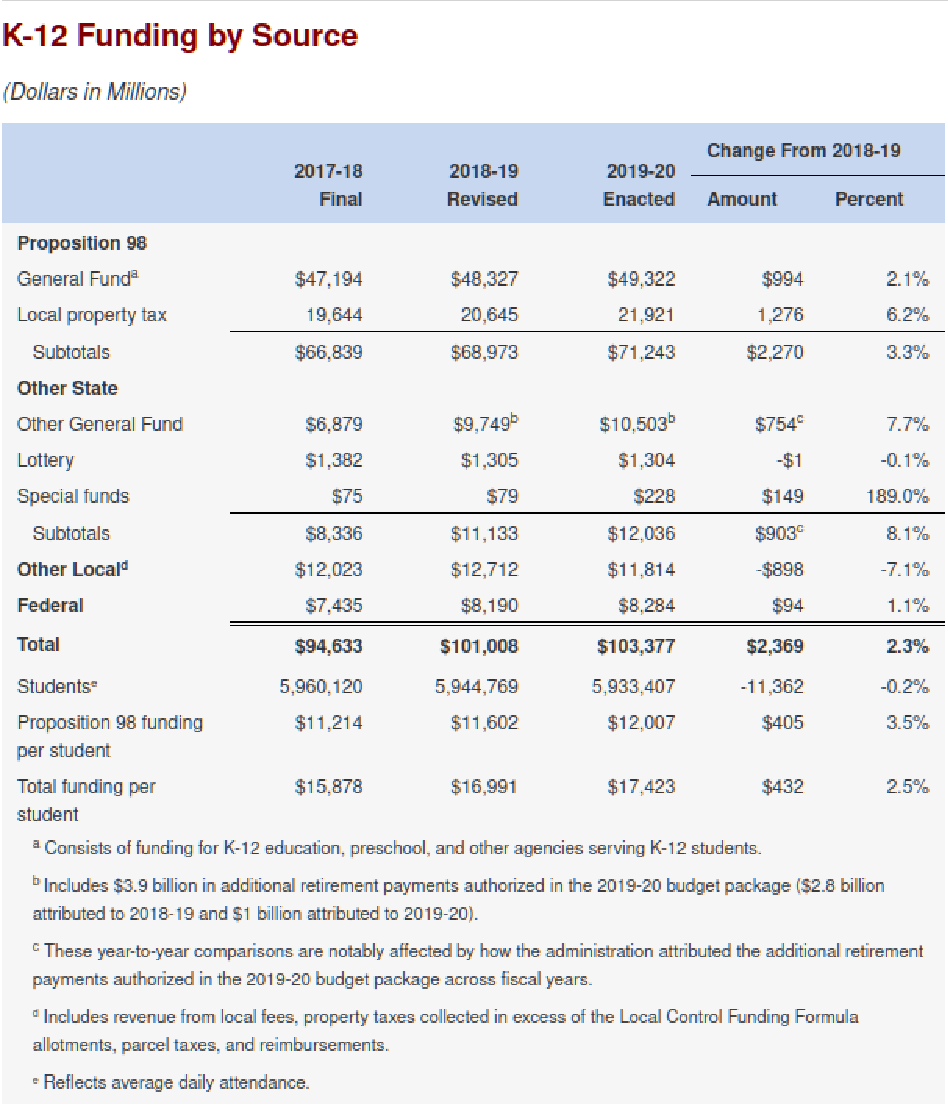
\includegraphics[width=\textwidth]{2019-20_K-12_Funding_by_Source.pdf}\\ %chktex 8
  \footnotesize\raggedright\textcite{LAO2021}.
\end{figure}

\prettyref{fig:2019–20_K–12_Funding} shows what money California has to fund its primary and secondary educational system, i.e.~grades K–12. This money is then allocated to local educational agencies (LEAs), through a formula known as the Local Control Funding Formula (LCFF).\footnote{The LCFF actually funds community colleges as well as public primary and secondary educational institutions, so it ought to be known as funding grades TK-14. Appoximately 89\% of LCFF funding goes to grades TK-12.} LEAs include individual charter schools, county offices of education, and local public school districts. The total amount of money for K–12 funding is allocated using a formula that was enacted by voters in 1988 \parencite{LAO2017}: Proposition 98. Prop. 98 was originally meant to be a minimum guaranteed funding level, but has evolved into a ceiling. The Legislative Analyst's Office (LAO), which serves as an independent, non-partisan research arm of the California Legislature in much the same way that the Congressional Research Service serves the U.S. Congress, calls Prop. 98 ``A Tale of Complexity''  (p.5) and says that ``A Plethora Tests and Rules Govern the Minimum Guarantee'' (p.5), and that ``State Has Made Myriad Adjustments to the Proposition 98 Calculations'' (p.5). Undoubtedly LCFF is complex, but LCFF is more transparent, has fewer rules, is more equitable, and is more responsive to the needs of public school districts that have a high proportion of under-served students than the Revenue Limit System that came before it. The Revenue Limit System was also complex, but in a completely difference way; it had many separately funded programs, called categorical programs, each with their own set of requirements, rules, durations, and funding levels. Each passing year saw more programs being added to the set of categorical programs until the entire collection became bnoth unwieldy and failed to equitably fund K-14 schools.

As seen in \prettyref{fig:2019–20_K–12_Funding}, Proposition 98 funding accounts for nearly 70\% of California's K–12 funding, the remainder coming from local property taxes and fees, and from various other federal and state sources. This money is distributed to county offices of education which then distribute it to public school districts. Districts then distribute funds to charter schools.

Some districts are funded outside of the LCFF system. These used to be called ``basic aid'' districts, but since the term is confusing, they are now called ``community funded'' districts. These are districts whose annual property tax revenue is greater than their annual LCFF entitlement. They get only ``basic aid'', i.e.~the constitutionally required minimum funding (the greater of \$120 per pupil or \$2,400 per district) from the state. For districts which are not community funded, the state contribution is the difference between a district's LCFF entitlement and its share of district property taxes. In other words, the state ensures that each district gets at least its LCFF entitlement, the total amount which is determined by Prop. 98.\footnote{An invaluable and comprehensive description of K-12 funding in California, for both public school districts and charter schools, can be found in \textcite{Aguinaldo.etal2022}, an annual publication.}

\subsection{Budgets \& Interim Reports}\label{sec:budgets}\indent

For a given fiscal year, which runs from July 1\textsuperscript{st} to June 30\textsuperscript{th}, the annual budget is the first of four important financial documents produced. Since budgets must be approved before the start of a fiscal year, they are actually produced and approved in the prior year.\footnote{Since a school's budget must be approved before the state budget is finalized, it is nearly cerain that a school's budget will need to be modified after it has been approved.} The next two financial documents are two (unaudited) interim reports, one in December, and another in March,  which track how well the school or district is adhering to the approved annual budget, and finally, after a certified public accountant has audited the school or district, a comprehensive annual financial report (CAFR) is produced in the fiscal year following the period it covers. State law requires that an independent auditor certify this retrospective account of the school or district's financial activity as being an accurate representation of the school's finances for the previous fiscal year.

\subsection{Local Control Accountability Plans (LCAPs)}\label{sec:lcaps}\indent

An important, recurring, non-financial report of schools is the Local Control Accountability Plan (LCAP). Although the LCAP is a three year plan, it is updated annually. The focus of an LCAP is on the programs that a school (public or charter) is going to implement, finance, and monitor that will allow it meet the goals that the state has set. These are goals that the California Department of Education sets periodically, primarily to ensure that students with the greatest needs are in fact served and are in addition to the seven goals that the Legislature set for charter schools in general.

Typically LCAP goals remain the same over their three year lifespan, but their financing may change if the metrics used to measure progress toward achieving those goals aren't showing progress. In unusual circumstances, how the goals are to be achieved might change. LCAPs are California's way of ensuring that all public schools, including charter schools, meet the same set of priorities or goals. Apparently, some LCAPs have been on the order of 500 pages long, although the norm is much less.

For each activity or group of activities, schools indicate what goal is being met, if the goal includes increased services for disadvantaged student, how well the school or district has met that goal, and how much money has been allocated to achieving and reporting those goals. (The reality of what the Department of Education wants is an order of magnitude more complicated than this description, but it is accurate as far as it goes.)

Unlike budgets and CAFRs, LCAPs don't have to ``add up'', nor do they have to offer a complete financial picture, but they do have to be consistent with other financial data. Expenditures have to be budgeted, and the amounts in a school's budget must agree with what's in the LCAP\@. The charter or public school's board must approve an LCAP at the same time as it approves its annual budget. % chktex 13

\subsection{Comprehensive Annual Financial Reports}\label{sec:CAFRs}\indent

A major source of financial data are the annual, independently audited, comprehensive financial statements of Rocketship Education. Comprehensive Annual Financial Reports (CAFRs) are sent to the California Department of Education (CDE) and to a charter's County Office of Education (COE) annually. They cover the previous fiscal year and are similar to annual budgets because they report the same information, perhaps in a different format. CAFRs are retrospective whereas budgets are prospective. The major difference is that CAFRs are independently audited and budgets are not. 

Similarly to bond underwriters, financial auditors are liable for ``omitting, misstating, or obscuring [items which] could reasonably be expected to influence decisions that the primary users make on the basis of those financial statements'' \parencite{Cayamanda2020}, and this requirement tends to increase the diligence of the auditors. However, potential liability doesn't always result in truly comprehensive financial statements; sometimes the lure of accounting fees overwhelms any misgivings, as was the case with Enron and Arthur Andersen in 2001, and apparently with Donald Trump in 2022. Errors and sloppiness may exist, but in general, fraud is thankfully rare, in part because fraud on the part of auditors would likely result in the loss of the auditor's license, effectively ending their business. 


\section{Charter School Financing}\label{sec:charter-school-financing}\indent

In California, charter schools are financed the same way as public schools are, from the same pot of money, using the same set of rules, except for one significant difference: how they finance facilities. Unlike public schools, charter schools have no taxing authority, so they cannot pass bond measures or parcel taxes. This lack of a taxing authority means that charter schools must either occupy existing public school facilities (potentially displacing existing public school students) or seek grants and donations to fund non-district facilities, either leased or purchased. The federal government provides significant amounts of facilities grant money and delegates to the states the administration of the program and the disbursement of the actual grants. 

An in-depth analysis of charter school finances requires a broader lens than one used for public schools because, in addition to all of the financial dealings of traditional public schools, almost all of which also apply to charter schools, charter schools have large and immediate needs for facilities that traditional public schools don’t have. This brings into the picture bonds, loans, grants, leases, construction, and the purchase and sale of real estate. Traditional public schools do issue several kinds of bonds, levy parcel taxes, and buy real estate on which they build schools, but they do so infrequently.Usually public schools have done this years ago, but charter schools have an immediately and reoccurring need for facilities. They face these needs once when they start up, and whenever they outgrow their facilities because of increased enrollment. These needs of charter schools for facilities and the financing associated with obtaining those facilities is more pressing, more immediate, and more common than the corresponding needs of traditional public schools whose enrollment doesn't fluctuate as much.\footnote{Usually a TSP sees a change in enrollment because of significant demographic changes like immigration or emigration, birth rate increases or declines. Charter schools can see enrollment changes absent any demographic change, even if the total number of students residing in a district staying the same. In some instances, increased enrollment in charter schools comes from public school students switching from the public school system to charter schools. This is what is happening to Oakland, CA and it produces simultaneous but opposite changes in enrollment.}

Once a charter has been granted the right to operate, it must file annually with the California Department of Education, just like public school districts, certain forms that detail its revenues and expenses. State law also mandates an annual audit by an independent accounting firm which charter schools must file with their County Office of Education. All together, these forms should provide a complete picture of a charter school's finances, and crucially, everything should be in agreement. Charters must approve and publish at a public meeting their annual budget, and they, just like traditional public schools, cannot spend unbudgeted money unless the governing board approves any changes at a public meeting.

\subsection{Charter Financial Documents}\label{sec:charter-financial-docs}\indent

There are numerous publicly available sources of charter school financial data. These are, in roughly chronological order, petitions/renewals, budgets, LCAPs,  interim financial statements, and finally, audited Comprehensive Annual Reports (CAFRs). \prettyref{tab:charter-fin-docs}, summarizes the financial reports which are available about charter school finances. The first two documents are specific to charter schools and have no public school equivalent.

\begin{table}[h]
  \centering\small%
  \caption[Charter School Financial Documents]{\textit{Charter School Financial Documents}}\label{tab:charter-fin-docs}%
  \begin{tabular}{llll}
    \toprule%
    \multicolumn{1}{c}{Name}  & \multicolumn{1}{c}{Description} & \multicolumn{1}{c}{Frequency} & \multicolumn{1}{c}{When} \\
    \midrule%
    Initial Petition  & Comprehensive description    & Once           & Before opening \\
    Renewal Petitions &  Similar to initial petition & Every 5 years  & Years 5, 10, 15, \ldots \\
    Budget            & Complete financial plan      & Annually       & Before June 15\textsuperscript{th} \\
    LCAP              & How to meet state priorities & Every 3 years  & With budget\\
    Interim Reports   & Current spending             & Twice yearly   & December, March \\
    CAFR              & Audited financials           & Annually       & In the following year \\
    \bottomrule%
  \end{tabular}
\end{table}%

Viewed chronologically, the first financial statement from a charter school is contained in their initial petition. Although petitions are not submitted under penalty of perjury, any material change to a petition would likely be cause for a re-evaluation of the petition, something that is undesirable from the charter's point of view. Petitions are presented at the start of a charter school's life and periodically thereafter, whenever their charter needs to be renewed. Petitions and renewals are discussed next.

\subsubsection{Petitions \& Renewals}\label{sec:petitions-renewals}\indent

Before a charter school is allowed to begin operation, every charter school in California is required to present to a chartering authority a petition which must contain certain required elements. The absence of one of these elements is grounds for denying the charter's petition to operate. For example, what is the intent of the charter school? How is the charter school going to measure its success or failure? What population is it targeting? And, what are its financial projections?

One of the required elements of any petition is a financial projection. Although no one expects a charter school (or any school for that matter) to prepare and adhere to a budget that exactly matches what's been projected, budgets are expected to be a reasonable appoximation of actual revenues and expenses.

Petitions run anywhere from a hundred or so pages to over a thousand. They contain a wealth of data on curriculum, demographics, pedagogy, discipline, teacher recruitment, and, of course, on the charter school's finances. Only a few financial statements are needed to get a good overall picture of a school's or district's finances. These are the enacted annual budget and interim reports, the audited Comprehensive Annual Financial Report (CAFR), parts of the Local Control Accountability Plan (LCAP), and for charter schools, the financial portions of their petitions.

Fortunately, these documents are all publicly available and could, if needed, be the subject of a California Public Records Act (CPRA) request. The CPRA is the California equivalent of the federal Freedom of Information Act (FOIA). Many of the documents mentioned in this dissertation are available from the California Departments of Education and Finance, or from the Santa Clara County Office of Education.\footnote{Since these documents are publicly available and may be freely copied, so no copyright is applicable, nor can one be claimed.}

Since Rocketship schools are all operated by a single entity, (currently) Rocketship Education, DBA Rocketship Public Schools, a 501(c)(3) non-profit, their financial statements and those of their affiliates are rolled up into a single document, the Consolidated Financial Statements and Supplementary Information. Every school is included in this single document, as are separate Launchpad Development LLC's that own facilities leased to individual schools. % chktex 36

\subsection{Other Data}\label{sec:other-data}\indent

Vast amounts of data are available from the federal, state and  local governments, easily over half a million datasets each containing anywhere from a hundred elements to a hundred thousand elements. Unfortunately these data have been collected in different formats, over different time periods, using different inclusion criteria, more or less carefully. Picking a subset of educational data to use and then cleaning it is a huge endeavor well beyond the scope of this dissertation. That being said, a very small subset of available datasets will be consulted, based on the immediate need at hand. The most likely datasets to be consulted are those maintained by:

\begin{itemize}
  \item California Department of Education and the State Board of Education
  \item The County of Santa Clara and the Santa Clara County Office of Education
  \item The California Open Data Portal
  \item National Center for Education Statistics (NCES) at the Institute for Education Sciences (IES)
  \item Stanford Educational Data Archive (SEDA)
  \item School Finance Indicators Database
  \item EdSource, Ed-Data, and other aggregators of educational data specific to California
\end{itemize}

\subsubsection{State and Federal Filings}\label{sec:state-federal-filings}\indent

Two filings are of particular interest: FPPC Form 700, Statement of Economic Interests, and IRS Form 990, Return of Organization Exempt from Income Tax. Both forms force the disclosure of personal financial information (Form 700) or personal financial information and business financial information (Form 990). 

Some officers of Rocketship may be required to submit annually to the California Fair Political Practices Commission (FPPC) Form 700, Statement of Economic Interests. This particular requirement of charter school officers is not settled law, but if Form 700 is filed, it will list the submitter's assets and income that are related to the position they hold in Rocketship Education or Launchpad Development. The intent is to prevent related-party transactions by enumerating an officer's economic interests so that a school can avoid doing business with entities that might benefit an officer. Rocketship's initial petition for Mateo Sheedy states that Form 700, Statement of Economic Interest, shall be filed by all board members, candidates for board membership, corporate officers, principals and assistant principals, among others. 

The federal Internal Revenue Service grants income tax exemptions to organizations that meets the requirements of §501(c)(3) of the  Internal Revenue Code.\footnote{26 USC 501, i.e. Title 26, Subtitle A, Chapter 1, Subchapter F Part I § 501(c)(3)} These organizations must file Form 990 annually that provides some minimal financial data. (Tax returns of for-profit organizations are not public documents and their contents do not have to be disclosed; however, in order to sell stock to the public, i.e.~to be listed on a stock exchange, firms are required to publish various financial documents, which like bond prospectuses, are required to be informative and complete.) %chktex 36

\subsubsection{Bond prospectuses}\indent

Bond prospectuses are also a source of financial information. When bonds are issued, they are  described in detail in a prospectus. These prospectuses, in addition to specifying the terms (e.g. interest rate, repayment schedule, collateral) of the bond, contain information relevant to assessing the risk associated with purchasing that bond.

Bond prospectuses can be mined for data that might not appear in petitions or financial statements because bond underwriters are ``potential liability for any material misrepresentations or omissions contained in a registration statement or prospectus'' \parencite{Block.etal2008}. This liability, of course, is not unlimited. If bond underwriters exercise due diligence or the misrepresentation is not material, the underwriters are probably not liable. Crucially, the definitions of \textit{material misrepresentation} and \textit{due diligence} depended on both statute and case law, so a bond underwriter can only make a reasoned guess at their exposure to liability. The result is that bond underwriters are likely to be more diligent that is absolutely necessary.

Unlike many studies, there is not a paucity of data on Rocketship, rather there is a surfeit. The data collected so far is voluminous. The current number of pages of initial and renewal petitions runs to 7371 pages for just Rocketship schools in Santa Clara County.\footnote{The massive size of some of these petition calls into question whether authorizers read them in their entirety.} Three bond prospectuses total over 1000 pages. And there are many financial data documents yet to obtain. For example, of the six categories of financial data listed in Table~\ref{tab:charter-fin-docs}, only half have been collected.

The challenge for this inquiry will be to organize the data so that gaps and anomalies can be identified, interesting and valid comparisons can be made with public schools and other charter schools, and the flows of money in and out of Rocketship can be identified. One approach would be to create a common framework and recast all the financial data from each school into that common framework. But, until the data have actually been collected and analyses started, choosing one particular framework within which to work is likely to lead to work which will need to be redone using a different framework.


\section{Real Estate}\label{sec:real-estate}\indent

Charter schools in California, as mentioned, do not have taxing authority, and so must finance – somehow – the facilities they plan to occupy before they receive any per-pupil state funding. As shown in \prettyref{tab:charter-facilities-options}, they have three options: lease, co-locate, or buy.

\begin{table}[htb]
  \centering\small%
  \caption[Charter School Facilities Options]{\textit{Charter School Facilities Options}}\label{tab:charter-facilities-options}%
  \begin{tabular}{ll}
    \toprule%
    Option    & Description \\
    \midrule%
    Lease     & The charter school leases from either a commercial entity or from a school district. \\
    Co-locate & A school district must provide reasonably equivalent facilities. \\
    Purchase  & The charter school buys existing facilities or builds their own. \\
    \bottomrule%
  \end{tabular}
\end{table}%

\subsection{Leasing}\label{sec:leasing}\indent

Charter schools may lease their facilities from either a related party, or at arms length, from an unrelated party. Terms and length of leases vary. If the lessor is an unrelated party, the charter schools may take advantage of grants offered by the Charter School Finance Authority authorized by California SB740\footnote{Ed. Code §47614.5 et seq. and CCR §10170 } ``to offset annual on-going facility costs for charter schools that service a high-percentage of students eligible for free or reduced-price meals (FRPM) or located in a public elementary school boundary serving a similar demographic'' \parencite{CATreasurer2023}. The amount of the grant is the lesser of the school's ADA × \$1,420 or the annual rent × 75\%\footnote{This is the basic calculation. As expected, there are variations and permutations, and these are enumerated in Section 6, Grant Award Calculations of the program's FAQ\@. The principle limitation is that the charter school must serve.} To be eligible, charter schools must ``service a high-percentage of students eligible for free or reduced-price meals (FRPM) or [be] located in a public elementary school boundary serving a similar demographic'' \parencite{CATreasurer2023}.

If the charter school is leasing from an related party, usually SB740 grants are not available. However, the definition of \emph{related party} does not include non-profit entities whose only business is supporting charter schools. For example, a non-profit charter school may lease a property from a related non-profit entity whose only business is owning and maintaining that property. This is the relationship that Rocketship Education has with the owners of the facilities they lease. The structure of Rocketship Education is diagrammed in \prettyref{fig:RSED-corporate-structure}.

\subsection{Co-Locating}\label{sec:co-locating}\indent



Tax credits are another potential source of profit. The New Markets Tax Credit is a 39\% tax credit, usable over seven years, available to those who make an investment in specified economically depressed neighborhoods. A 39\% tax credit is roughly twice the current corporate tax rate which means that this credit wipes out the taxes on gains equal to twice the initial investment (which also has a return). 

The NewSchools Venture Funds, the Charter School Fund, and the Charter School Growth Fund are just a few examples of venture funds that specialize in charter schools. Since it is unlikely that investors will invest in a fund that does not return a profit, establishing exactly how these funds turn a profit is going to be a key goal of this study's explorations.\footnote{It is interesting that none of the web sites of these funds mentions that fund's return on investment (ROI). The absence of any indication of a return on investment is either an innocent mistake or much more likely, an attempt at obfuscation.}


\section{Are There Gaps or Anomalies in the Data?}\label{sec:gaps-anomalies}\indent

All of the sources mentioned above should be in basic agreement, i.e.~the LCFF funding received by a Rocketship charter school should match what the state thinks it's sending to the school, what the school reports to the state it received and spent, what independent auditors report the school received and spent, and what it actually spent. Further, bond prospectuses and Security Exchange Commission (SEC) filings should be in agreement with themselves and with budgets. If these figures are not in agreement, something is amiss and should be investigated.

In some fashion or another, all profit must originate from Rocketship's revenue. In the case of the sale-leaseback of facilities, for example, the rent over and above market rates constitutes profit to the property owners, and this is an operational expense ultimately paid for by tax payers. If facilities are bought with public dollars (i.e.~federal grants) and subsequently sold, the net proceeds are profit that might accrue to an organization other than Rocketship. If technology is being used and the contracts are not at arm's length, then someone or some organization is making more than the usual profit. If student data is being sold by a for-profit entity that operates non-profit charter schools, that's revenue that rightfully belongs to the students or to the non-profit schools. 

Determining whether there are gaps or anomalies in a charter school's financial data is time-consuming but not very complex. When examining financial statements, one should be alert to unusual year-to-year changes, ratios (e.g. salaries to total expenses) that are markedly different from the norm, entries that are missing components, or entries that are not supported by detail elsewhere. Complex third-party transactions that don't seem to add value are also indicators that further investigation is needed.

In the search of gaps or anomalies, one might ask questions such as:
\begin{itemize}
\item Are the data available and accessible? Charter schools are notorious for simply not filing required documents or filing them horrendously late, or submitting documents that are incomplete. Petitions are not usually a problem because without a petition, or with a materially incomplete petition, the petition will not be granted. However, once a school is operational, late or missing filings will not bring everything to a halt. Although Rocketship was fined for failing an attendance audit, it was allowed to continue to operate.
  \item Have the data been misrepresented? There are forensic techniques (e.g. Benford's Law) that can point to suspect data \parencite{Zhu.etal2021}. There is also triangulation which involves comparing one source of data with another to see if they match. For example, charter petitions make forecasts of revenue and expenses. How accurate were those forecasts? Were the reasons given for anomalies plausible? foreseeable? reasonable? Following Hanlon's Razor\footnote{``Never attribute to malice that which is adequately explained by stupidity.'' Naturally, Hanlon's Razor follows Stigler's Law of Eponymy: ``No scientific discovery is named after its original discoverer.'' Stigler's Law adheres to Stigler's Law.}, a single anomaly is not usually a sign that something is being covered up, but several persistent anomalies usually are. %chktex 12 38
  \item California requires that LEAs meet the numbers they previously forecast or explain why they didn't meet those numbers. Were those goals met, and if not, were the reasons proffered legitimate? When preparing a budget, LEAs must also certify they can meet their financial obligations for the current year, and for the next two years. If an LEA cannot certify that they can, they might receive a visit from the California Department of Education's Financial Crisis \& Management Assistance Team (FCMAT), and in the extreme case be subject to a state takeover or to involuntary closure. 
\end{itemize}%

\subsection{Triangulation}\label{sec:triangulation}\indent

Another technique for determining if there are gaps or anomalies is to use triangulation. Triangulation is the use of multiple sources of data. While triangulation in social science research often refers to the mixed methods use of quantitative and qualitative methodologies, the common definition refers to the analysis of multiple forms of corroborating evidence in the form of financial and media documentation. For example,  \textcite{Bhandari2022} notes that one of the forms of triangulation is ``[u]sing data from different times, spaces and people'' and also that ``[t]riangulation in research means using multiple datasets, methods, theories and/or investigators to address a research question. It’s a research strategy that can help you enhance the validity and credibility of your findings.''\footnote{Triangulation does not imply exactly three concepts or ideas; often, as is in this dissertation, more than three concepts, ideas, data are combined in the analysis.}


\section{Are There More Serious Financial Issues?}\label{serious-problems}\indent

Unfortunately, charter schools and charter school chains have a long history of various kinds of fraud. \textcite{Lafer2017}, \textcite{ITPT2018}, \textcite{Burris.etal2020}, and \textcite{Burris.Bryant2020}, are just a few of the reports that detail fraud and waste in charter schools. Although Rocketship has engaged in a number of questionable activities, it has not been charged anything illegal.\footnote{Rocketship schools in Santa Clara have had ties with a virtual charter school serving special education students hundred of miles away. They have collected pandemic-relief funds intended for businesses and not available to public schools. Rocketship has been the subject of several Letters of Concern from the California Department of Education, and it has had petitions to open schools denied for substantive reasons. Many of these issues have been collected and can be viewed at \url{https://www.scoop.it/topic/charter-choice-closer-look} \parencite{Marachi2022}.} But with billions of dollars allocated to charter schools for facilities in the last 15 years in California alone \parencite[4]{Lafer2017}, coupled with lax or no oversight, the temptation to misappropriate funds must be strong. It is also instructive to note that Californian charter schools have fought tooth and nail to prevent any laws that would increase transparency or hold charter operators to the same conflict-of-interest standards that public schools and other government entities are held to. While the charter sector has for the most part been successful in warding off demands for accountability, the Attorney General of California issued an official ruling in 2018 stating that the Brown Act, the CPRA, and Government Code §1090 apply to charter schools as well as to other LEAs \parencite{Becerra.Medeiros2018}.

However, it's not necessary to misappropriate funds to make money off of charter school facilities. As the report \citetitle{ITPT2018} from \citeauthor{ITPT2018} details,

\begin{quotation}\noindent\OnehalfSpacing%
While charter schools constructed with general obligation bonds cannot be sold or used for anything other than the authorized school, schools constructed with tax-exempt conduit bonds become the private property of the charter operator. Even if the charter is revoked, neither the state nor a local school district can take control of this property. Additionally, schools constructed with private funding subsidized by New Market Tax Credits or acquired with private funds but whose mortgage payments are reimbursed through the Charter Facilities Grant Program (known as “SB740”) are typically owned without restriction.\\ \sourceatright{\parencite[6]{ITPT2018}}
\end{quotation}

Rocketship has issued just shy of \$90M of tax-exempt bonds to ``finance and/or refinance the acquisition, construction,
expansion, remodeling, renovation, improvement, furnishing and equipping of the land and facilities''  \parencite{CSFA2015,CSFA2015a,CSFA2016,CSFA2017,CSFA2017a}. These conduit bonds are exactly the kind referenced in \textcite{ITPT2018}. The properties owned or leased are (partially) paid with public funds but are privately owned.

\subsection{Analyzing Rocketship's Bond Financing}\indent

Bond financing can be both complicated (a hard problem, but solution methods exist) and complex (many unknowns and interrelated factors). Illustrating this are two examples of the analysis from just a single prospectus, that of Rocketship's \$42M bond offering. That offering is described in the 536 pages which comprise \citetitle{CSFA2017a}. The \$42M offering is complicated because there are many moving parts which are described in the offering in the well-known language of bond finance. Terms, rates, contingencies, amounts, dates, and required performance are all specified in a fashion that has withstood legal onslaught many times over. But the offering is also complex because it must also convince others that its predictions are reasonable. The most important of those predictions is that the issuer can pay the interest and repay the principal when they due.

\prettyref{fig:flow_of_funds_overview} gives the overall picture and shows how rents from schools (blue) are ``intercepted'' by the California Controller (red) and paid directly to landlords, or paid into the Gross Revenue Fund (red) from which the Master Trustee pays lessors (orange) and bond holders and expense accounts (orange). What is not shown is the \$750 per ADA (in 2017, rising to \$1,211 in 2020–21) that Rocketship will apply to lease payments. Since money is fungible, the State of California is giving Rocketship between \$2.4 and \$3.7M depending on the year, money they would otherwise not have. This is effectively profit.

\begin{figure}[hbt]
  \centering
  \caption[Flow of Funds: Overview]{\textit{Flow of Funds: Overview}}\label{fig:flow_of_funds_overview}
  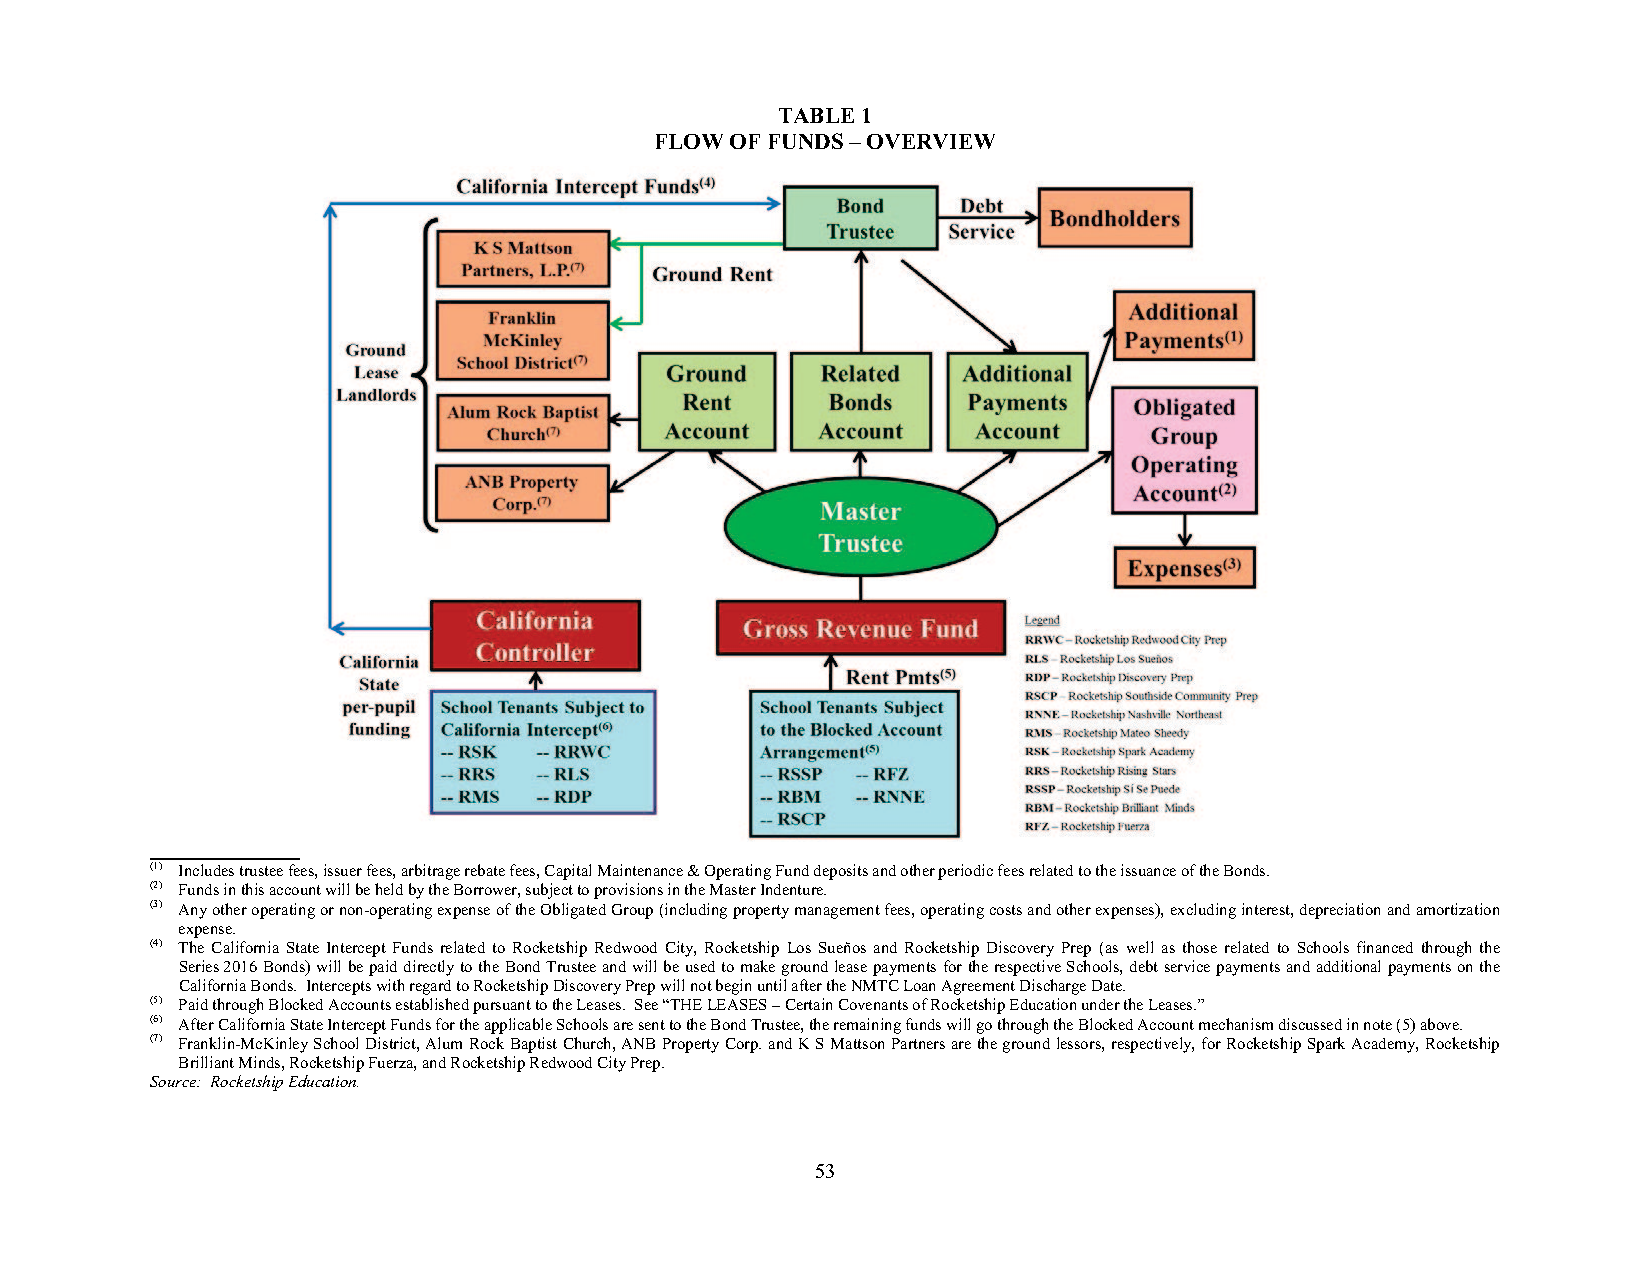
\includegraphics[width=\textwidth]{Flow_of_Funds_Overview}\\
  \footnotesize\raggedright\textcite[53]{CSFA2017}. 
\end{figure}

The next figure, \prettyref{fig:flow_of_funds_cross-collateralization} adds an important detail: how Rocketship uses its assets as collateral more than once.\footnote{\textit{Cross-collateralization} means using an asset as collateral for two or more obligations, here lease and bond payments.} In this case, if the payments of ``School Tenants'' are insufficient, the Master Trustee may require additional monthly payments from the ``Obligated Group Representatives and Member'' to supplement those from ``School Tenants''. 

\begin{figure}[hbt]
  \centering
  \caption[Flow of Funds: Cross-Collateralization]{\textit{Flow of Funds: Cross-Collateralization}}\label{fig:flow_of_funds_cross-collateralization}
  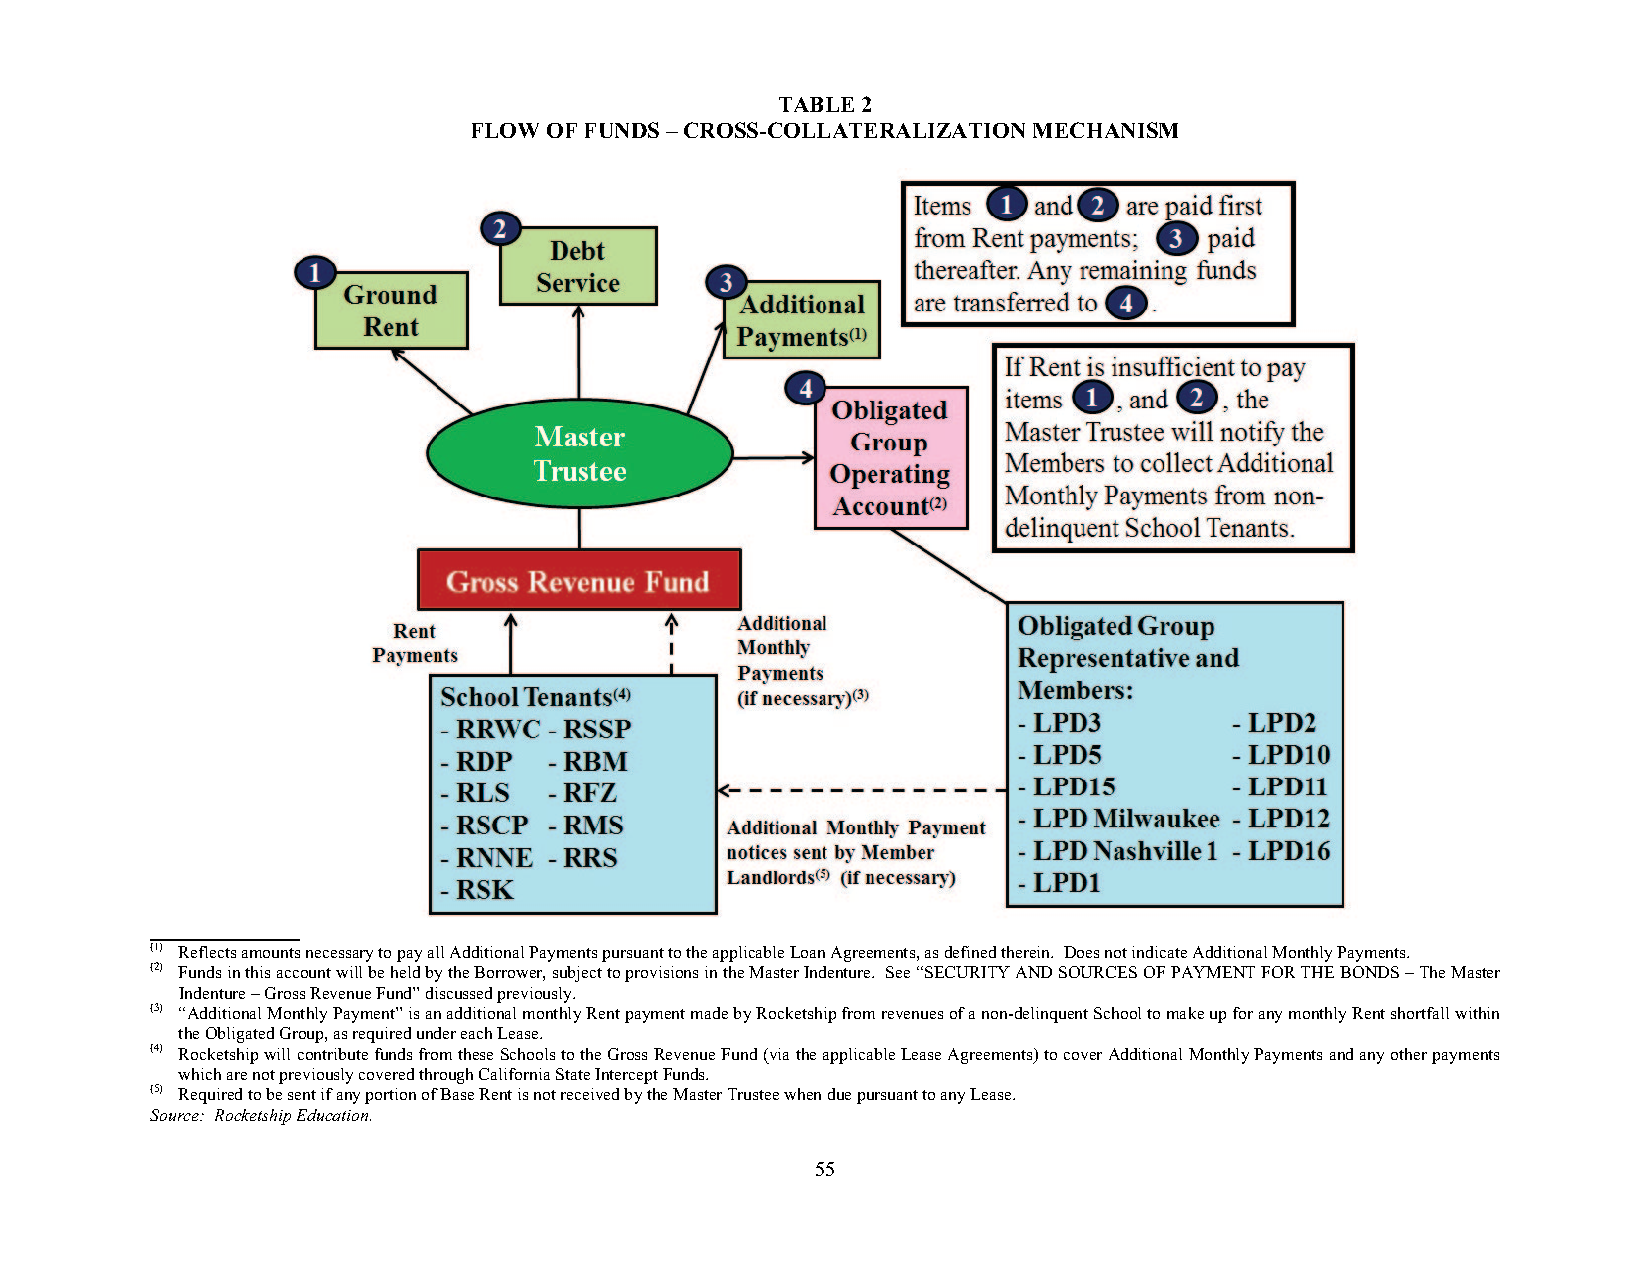
\includegraphics[width=\textwidth]{Flow_of_Funds_Cross-Collateralization}\\
  \footnotesize\raggedright\textcite[55]{CSFA2017}.
\end{figure}

These two examples show the kind of analysis that is needed to characterize a bond offering.


\section{The Flow of Money Through Rocketship?}\label{sec:flows-of-money}\indent

Since a goal of this dissertation is to map the flow of money into and out of Rocketship, I will use diagrams similar to the one used by \citeauthor{Baker.Miron2015} (\citeyear{Baker.Miron2015}), which is reproduced here as Figure~\ref{fig:opresflows}.
\begin{figure}[ht]
  \centering
  \caption[Operating Resource Flows]{\textit{Operating Resource Flows}}\label{fig:opresflows}
  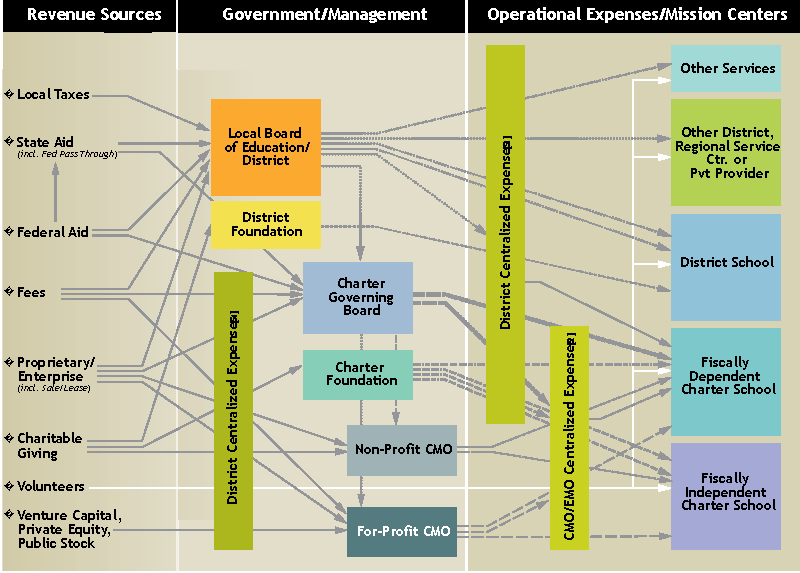
\includegraphics[width=\textwidth]{Operating_Resource_Flows}\\
  \footnotesize\raggedright\textcite[16]{Baker.Miron2015}.
\end{figure}
In this example, money flows from left to right, and there are no loops. Colors are used merely to distinguish the various blocks.

%%% Local Variables:
%%% mode: latex
%%% TeX-master: "Rocketship_Education-An_Exploratory_Public_Policy_Case_Study"
%%% TeX-command-extra-options: "-recorder"
%%% End:
                       % Chapter 3
\clearforchapter% %%% Time-stamp: <2023-06-14 16:04:13 vladimir>
% %%% Copyright (C) 2019-2023 Vladimir G. Ivanović
% %%% Author: Vladimir G. Ivanović <vladimir@acm.org>
% %%% ORCID: https://orcid.org/0000-0002-7802-7970

\chapter{Findings}\label{ch:results}\noindent
\bigskip%

This chapter discusses the result of exploring answers to my research question: Has Rocketship structured itself and its finances, to earn a return to investors, focusing especially on real estate transactions, and if so, how?

\section{Rocketship Education and Related Entities}
\subsection{Rocketship Public Schools (née Rocketship Education)}
\begin{enumerate}
  \item Articles of Incorporation
\end{enumerate}
\subsection{Launchpad Development LLC}
\begin{enumerate}
  \item Articles of Incorporation
\end{enumerate}

\subsection{Rocketship's Corporate Structure}\label{sec:rocketship-corp-struct}\indent


\begin{figure}[ht]
  \centering
  \caption{\normalfont\emph{The Corporate Structure of Rocketship's Santa Clara County Schools}}\label{fig:RSED-corporate-structure}

%   \mbox{}\begin{forest}
%   for tree={
%     % style of nodes
%     draw = black, semithick,
%     font = \sffamily,
%     text width = 18mm, text badly centered, % <-- "align=center" doesn't work
%     inner sep = 3mm,
%     % style of tree (edges, distances, direction)
%     parent anchor = south,
%     parent anchor = south,
%             grow' = south,
%              edge = teal!50,
%     forked edge,            % for forked edge
%             s sep = 4mm,    % sibling distance
%             l sep = 8mm,    % level distance
%          fork sep = 4mm,    % distance from parent to branching point
%          tier/.option=level,
%        }
%        [ Rocketship Education,
%       [ Rocketship Support Network (RSN) ]
%       [ Rocketship Mateo Sheedy Elementary (RSM) ]
%       [ Rocketship Sí-Se-Puede Academy (RSSP) ]
%       [ Rocketship Los Sueños Academy (RLS) ]
%       [ Rocketship Mosaic Elementary (ROMO) ]
%       [ Launchpad Development Company
%         [ Launchpad (LP) ]
%         [ Launchpad Development One LLC (LLC1) ]
%         [ Launchpad Development Two LLC (LLC2) ]
%         [ Launchpad Development One LLC (LLC3) ]
%         [ Launchpad Development One LLC (LLC4) ]n
%       ]]
%     ]
% \end{forest}
    % \begin{forest}
    % for tree={grow'=0,folder,draw,align=left}
    % [root
    %   [A
    %     [one line]
    %     [one line]
    %     [two\\ lines,text width=25ex]
    %     ]
    %     [B
    %     [one line]
    %     [another line]
    %     ]
    %   ]
    % \end{forest}
    \scriptsize
    \sffamily
  \begin{forest}
    for tree={grow'=east, folder, draw, align=left}
    [ \textbf{Rocketship Education}, baseline
      [ Launchpad Development Company
        [ Launchpad (LP) ]
        [ Launchpad Development One LLC (LLC1) ]
        [ Launchpad Development Two LLC (LLC2) ]
        [ Launchpad Development Threee LLC (LLC3) ]
        [ Launchpad Development Four LLC (LLC4) ]]
      [ Rocketship Support Network (RSN) ]
      [ Rocketship Mateo Sheedy Elementary (RSM) ]
      [ Rocketship Sí-Se-Puede Academy (RSSP) ]
      [ Rocketship Los Sueños Academy (RLS) ]
      [ Rocketship Mosaic Elementary (ROMO) ]]
    \end{forest}
\end{figure}
    
\section{Rocketship Locations and Property Information}
\begin{table}[thb]
  \caption[Rocketship Property Information]{\textit{Rocketship Property Information}}\label{tab:RocketshipLocations}\SingleSpacing%
  \begin{tabular}{lll}
    \toprule
    School          & Address                               & Property Information \\
    \midrule
    Mateo Sheedy    & 788 Locust St., San José, CA 95110    & \prettyref{sec:mateo-sheedy-info} \\
    Sí Se Puede     & 2249 Dobern Ave, San José, CA 95116   & \prettyref{sec:sí-se-puede-info} \\
    Los Sueños      & 331 S. 34th St, San José, CA 95116    & \prettyref{sec:los-suenos-info} \\
    Discovery Prep  & 370 Wooster Ave, San José, CA 95116   & \prettyref{sec:discover-prep-info} \\
    Mosaic          & 950 Owsley Ave, San José, CA 95122    & \prettyref{sec:mosaic-info} \\
    Brilliant Minds & 2960 Story Rd, San José, CA 95127     & \prettyref{sec:brilliant-minds-info} \\
    Alma Academy    & 198 West Alma Ave, San José, CA 95110 & \prettyref{sec:alma-academy-info} \\
    Spark Academy   & 683 Sylvandale Ave San José, CA 95111 & \prettyref{sec:spark-academy-info} \\
    Fuerza          & 70 S. Jackson Ave, San José, CA 95116 & \prettyref{sec:fuerza-info} \\
    Rising Stars    & 3173 Senter Road, San José, CA 95111  & \prettyref{sec:rising-stars-info} \\
    \bottomrule
  \end{tabular}
\end{table}

\subsection{Property Acquisition Timeline}

\section{The Data}
\begin{enumerate}
  \item What is the actual price, date, and buyer \& seller information for each property?
  \item What is the legal relationship between Rocketship Education and Launchpad Development?
  \item How were Rocketship facilities in Santa Clara County financed?
  \item What are the type and terms of all bonds.
  \begin{enumerate}
    \item What bonds were floated: type, rate, \& terms; guaranteed by whom or how? \\
    \noindent Since these are securities, their prospectuses are filed with the Securities Exchange Commission, and I assume that info is on their web site.
    \item For conduit bonds, look on the California Department of Education or Department of Finance web sites.
  \end{enumerate}
  \item Enumerate all known leases and their terms. Was part of the lease payment paid by California?
  \item Enumerate all known loans.
  \begin{enumerate}[a.]
    \item What was used as collateral? 
    \item What were the terms?
  \end{enumerate}    
  \item Enumerate donations from foundations and individuals.
  \item Enumerate venture fund investments.
\end{enumerate}

These data represent the monies that are flowing into Rocketship/Launchpad related to facilities, real estate, bonds, loans, and donations and not tied to the number of students. Once that's been assembled, roll up into one spreadsheet, Rocketship's consolidated financial statements for the fourteen years (2008--2022). The consolidated financial statements can then be compared against the known real estate, bond, loan, and donation transactions. Noe where data is missing or where it conflicts with the consolidated financial statements.

Forms which have been filed with a government entity:
 \begin{enumerate}
  \item Federal 990 forms to check against financial statements. IRS maintained. Should cross-reference the financial statements.
  \item Annual and interim budgets submitted to the California Department of Education.
  \item Petition approvals and renewals submitted to local school districts, the SCCOE, or the California State Board of Education.

  The Santa Clara County Office of Education (SCCOE), and each school district in which Rocketship petitioned to open a school has some data/notes from one or more board meetings in which the petition or renewal was discussed. These data might have been presented by Rocketship or by county or district staff. Sometimes there is also public comment.
  
Often, petitions presented to a school district have been denied and appealed to the Santa Clara County Board of Education, and in a few cases, to California's State Board of Education.
  
  \item There is some published material on Rocketship.
  \begin{enumerate}[a.]
    \item Some books have been written about Rocketship
    \item Roxana has two ScoopIt collections on Rocketship on and charter schools.
    \item The ``Stop Rocketship'' web site has lots of information on Rocketship.
    \item Several academics have datasets of school or district financial information  which include Rocketship.
    \item Numerous articles, web sites, and blog postings include Rocketship financial data.
  \end{enumerate}
  \item Other, outside entities that may add revenue to Rocketship
  \begin{enumerate}
    \item Zeal
    \item Dreambox Learning
  \end{enumerate}
\end{enumerate}

%%% Local Variables:
%%% mode: latex
%%% TeX-master: "Rocketship_Education-An_Exploratory_Public_Policy_Case_Study"
%%% End:
                      % Chapter 4
\clearforchapter%%% Time-stamp: <2022-05-13 21:56:25 vladimir>
%%% Copyright (C) 2019-2022 Vladimir G. Ivanović
%%% Author: Vladimir G. Ivanović <vladimir@acm.org>
%%% ORCID: https://orcid.org/0000-0002-7802-7970

\chapter{Discussion}\label{ch:discussion}

\begin{comment}
\section{Judging Case Studies}\label{sec:case-studies}

\subsection{Validity}
  \subsection{Reliability}
  \subsection{Limitations}
  \section{Evaluating the Results}
  \section{Rival Explanations}
  \section{Future Research}
\end{comment}

%%% Local Variables:
%%% mode: latex
%%% TeX-master: "Rocketship_Education-An_Exploratory_Public_Policy_Case_Study"
%%% End:
                    % Chapter 5
\newpage%

\setlength{\afterchapskip}{0.8\onelineskip}

\OnehalfSpacing%
\setlength{\bibitemsep}{\onelineskip}
\printbibliography{}

\DoubleSpacing%
\appendix%
\part*{Appendices}
\begin{appendices}
\chapterstyle{appdx_sjsu}
\clearforchapter%%% Time-stamp: <2023-05-23 10:22:24 vladimir>
%%% Copyright (C) 2019-2023 Vladimir G. Ivanović
%%% Author: Vladimir G. Ivanović <vladimir@acm.org>
%%% ORCID: https://orcid.org/0000-0002-7802-7970
\chapter{School Financing in California}\label{ch:ca-school-financing}

This appendix presents an example of public school financing in California.\footnote{For a more detailed look at what a complete budget document looks like, see ``LASD 2022–23 Annual Budget'' of Item H.4 of the June 13, 2022 LASD Board Meeting (\url{https://tinyurl.com/lasd-2022--23-annual-budget}). Note that most public school budget documents are not as comprehensive or as well put together as LASD's are.} %chxtex 8
Understanding the normal, usual, default financing of schools in California is necessary in order to be able to identify where Rocketship's might differ. The description which follows is necessarily high-level; the budget document for 2022–23 that LASD submits to SCCOE and hence to the state runs to 118 pages of unadorned tables derived from accounting spreadsheets.

First, the highest possible level look at a LASD budget is presented. This is the \textit{All Funds Summary}. Next are five tables that delve one level down from the \textit{All Funds Summary}. Each of those tables can be further decomposed until individual SACS accounting (object) codes are reached. SACS code reflect exactly one kind of expenditure or revenue. For example, money received from the Federal Emergency Management Agency (FEMA) is recorded under SACS object code 8281 and no where else. How that money is spent is recorded under object code 8285. The lowest level of accounting is money received or money paid. All money received goes into at least one fund and is recorded under at least one object code. Payments are handled correspondingly. The intent of this process is to record unambiguously and completely every monetary transaction. 

Public school districts and charter schools receive funding from the state and the federal governments which most often goes into a district's or school's General Fund. A portion of funding is restricted to particular programs, and sometimes that money goes into a specialized and restricted fund, but the norm is for the General Fund to account for the majority of transactions.

The first table to look at is the aggregate of all funds as shown in \prettyref{fig:LASD_All_Funds_Summary}. It is a very high-level summary of a school's or a district's budget. It's a snapshot of what the district's revenues are expected to be, roughly where that revenue is expected to come from, what the district's expenses are expected to be, and whether revenue and expenses are expected to be in balance. It is the rough equivalent of a business income statement.\footnote{Schools group their finances by funds. Most of their revenue goes into the general fund, and most of their expenses come out of the general fund. Some transactions must by law be accounted for in different funds. The three largest funds are the General Fund, the Special Revenue Fund, and the Capital Projects Fund, and together they account for virtually all of the financial activity of LASD.\@ Other schools may have a different set of funds, but all contain a General Fund that is the primary fund for their day-to-day financial activities.}

\begin{figure}
  \centering
  \caption[LASD 2019–20 All Funds Summary]{\textit{LASD 2019–20 All Funds Summary}}\label{fig:LASD_All_Funds_Summary}
  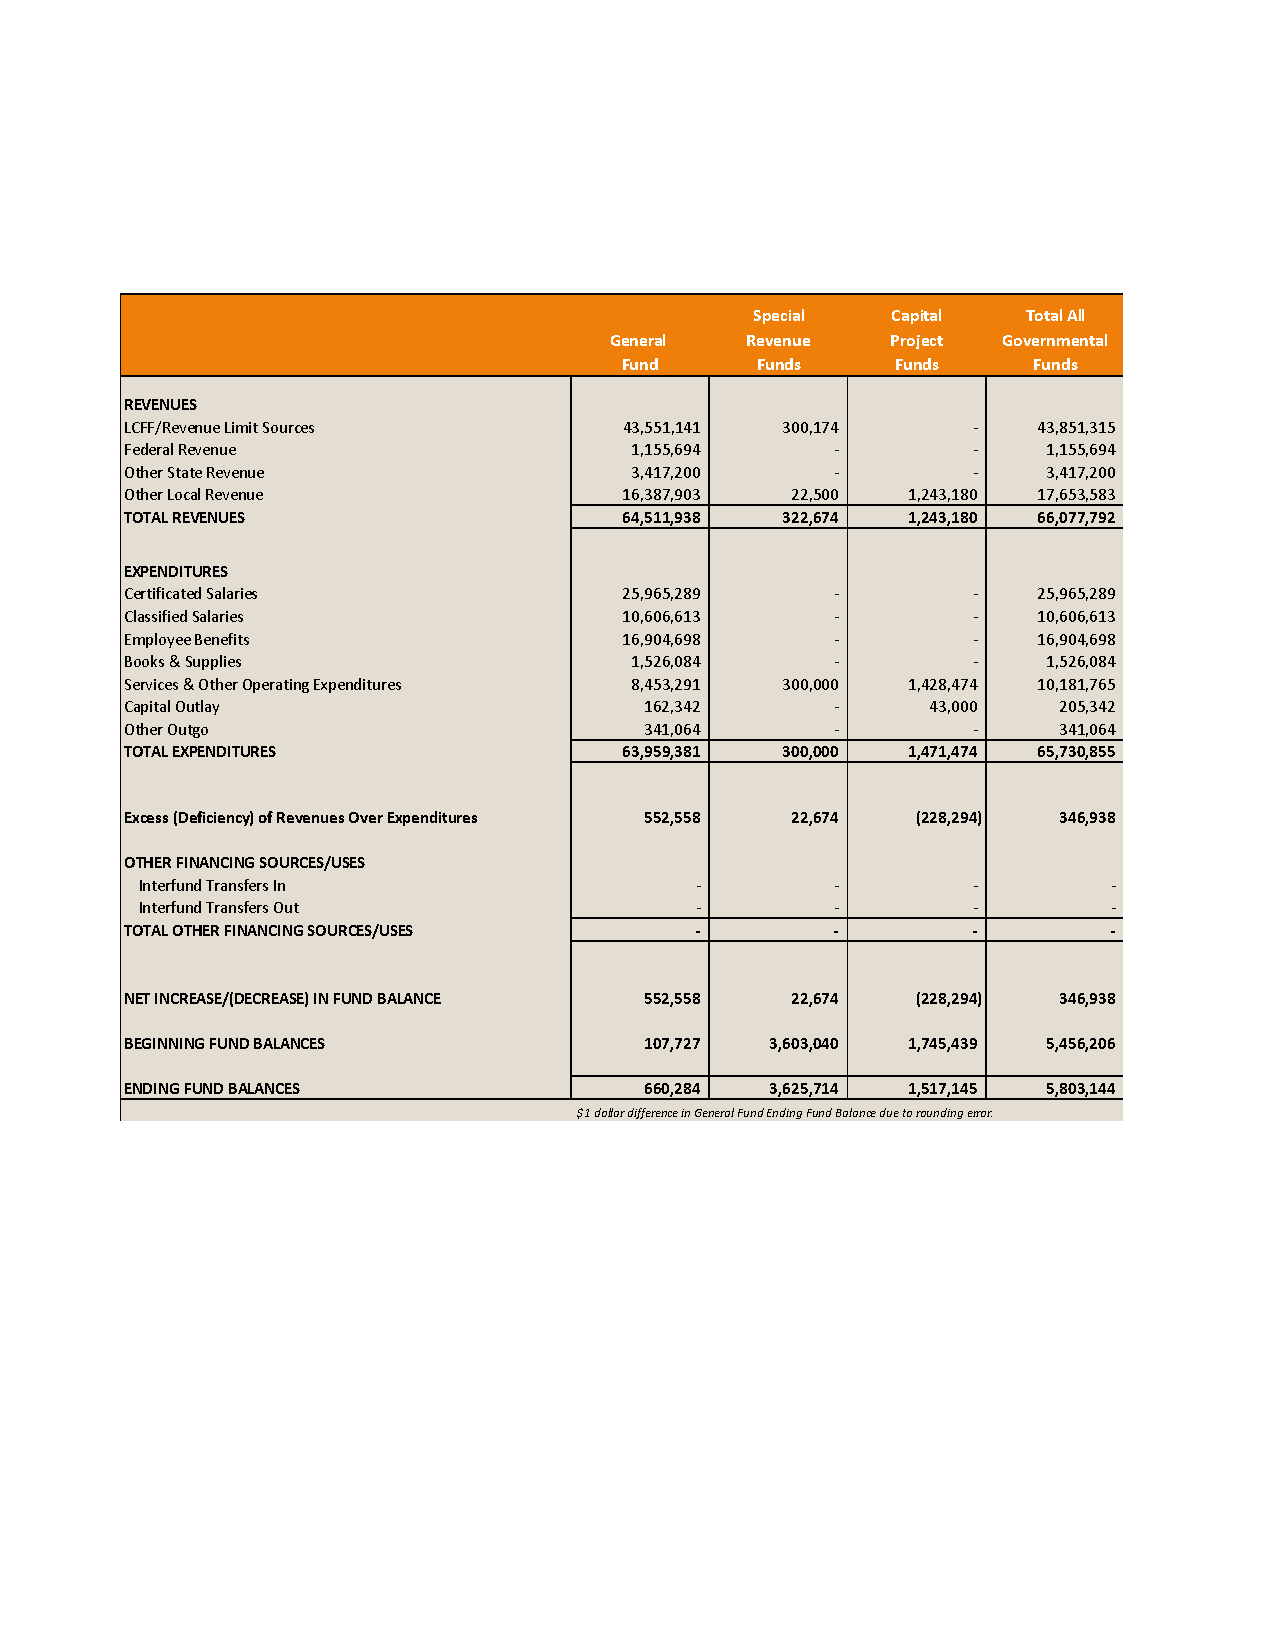
\includegraphics[width=\textwidth]{LASD_2019-20_All_Funds_Summary}\\ %chktex 8
  \footnotesize\raggedright\textcite[38]{Kenyon2019}.
\end{figure}

Because Figure~\ref{fig:LASD_All_Funds_Summary},~\titleref{fig:LASD_All_Funds_Summary}, is a snapshot, detecting unusual changes year-to-year is not possible. Changes are detectable using  \prettyref{fig:net-position} which compares fiscal two years. However, with just a budget summary, one can nonetheless note some interesting ratios, for example, the percentage of expenses spent on salaries and benefits. For LASD in 2021–20, this is 80.18\% which is in line with what is typical of elementary school districts in California. One can calculate the state-wide average for all districts for 2019–20 using the Data Table at \url{www.ed-data.org/state/CA}, and that comes out to 83.71\%. So, LASD spends a little less on salaries and benefits than the average elementary school district in California does.

Calculating this ratio brings up a general issue: What is an appropriate comparison group? In this particular case, the Ed-Data web site does not have county-level financial data, so the only comparison which can easily be made is at the state level. But should the state-level comparison group be all districts, or just elementary school districts? Should ``basic aid'' districts, also called ``community-funded'' districts, districts whose property tax revenues exceed their LCFF entitlement, be included or not? Again, the Data Table tab on \url{www.ed-data.or/state/CA} does not filter by type of district (although the Graph tab does), so, in this case, using just the Ed-Data data, our choices are forced since we cannot use state-level data.

The other common financial business report is the balance sheet, which identifies assets and liabilities. In the educational world, this is the statement of net position. \prettyref{fig:net-position} shows LASD's assets and liabilities at the end of the 2019–20 school year. Note that unlike a balance sheet, a statement of net position for schools (and other governmental entities) does not balance; assets are not exactly equal to liabilities.\footnote{Business accountants achieve this seemingly low probability equality by adding a fudge factor, \textit{owner's equity}, so that \texttt{\textit{assets = liabilities + equity}} always, exactly.}

As an example of a number which stands out and is therefore worth investigating, is the large increase in Capital Assets, year over year, an increase of \$132M (line 3 of \prettyref{fig:net-position}). In \citetitle{Kenyon2021}, six notes appear immediately after Figure~\ref{fig:net-position}, and these provide an explanation for the increase: LASD purchased a property whose cost was \$134.9M net of \$2.7M in depreciation. This purchase shows up again in line 1 of \prettyref{fig:Capital_Assets} and explains the enormous 9052\% increase in the value of LASD's largest asset in FY2019, land.

In addition, the \citetitle{Kenyon2021} contains a section, on pp. 19–45, called \textit{Notes to the Basic Financial Statements}. Theses notes are an integral part of the certified, audited annual statement, just as they are in audited financial reports in the business world; they cannot be omitted, and must be accurate and complete.  Note 7B of \textcite[7]{Kenyon2021}, General Obligation (GO) Bond Anticipation Notes (BANs), explains how LASD uses a common
technique to convert general obligation bonds into cash: issue BANs, backed by general obligation bonds, and payable when those GO bonds are issued.\footnote{One reason this makes sense is that interest rate on BANs is less than the interest rate of GO bonds, so LASD makes money by issuing BANs to pay off GO bonds. In a different situation, school districts issue tax revenue anticipation notes (TRANs) because property taxes are paid by taxpayers semi-annually and salaries are paid monthly, so districts often and predictably do not have the cash on hand to pay their employees. The solution is to issue TRANs backed by anticipated revenue, and are paid off when the school or district receives the funds.}

It's important to remember is that although changes in finances can be complicated, they should also be adequately explained in a transparent and complete CAFR\@. When the documents are incomplete or opaque is when serious concerns should be raised. % chktex 13

Within a CAFR are five summaries of financial tables that go one level deeper than the All Funds Summary. These are
\begin{itemize}\OnehalfSpacing%
    \item Summary of Net Position (\prettyref{fig:net-position})
    \item Change in Net Position  (\prettyref{fig:Change_Position})
    \item Net Costs of Services   (\prettyref{fig:Cost_Services})
    \item Capital Assets          (\prettyref{fig:Capital_Assets})
    \item Long-term Liabilities   (\prettyref{fig:Long-term_Liabilities})
  \end{itemize}

\begin{figure}
  \centering
  \caption[LASD YE 2020 Summary of Net Position]{\textit{LASD YE 2020 Summary of Net Position}}\label{fig:net-position}
  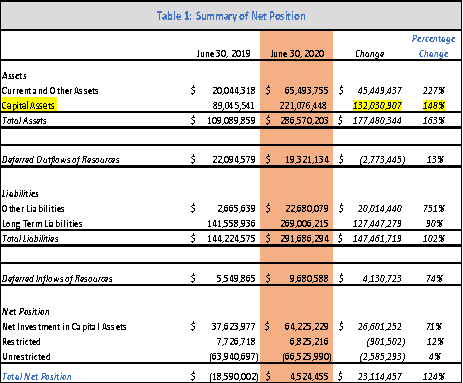
\includegraphics[width=\textwidth]{CAFR-YE2020_Summary_of_Net_Position}\\
  \footnotesize\raggedright\textcite[6]{Kenyon2021}.
\end{figure}

\begin{figure}
  \centering
  \caption[LASD YE 2020 Change of Net Position]{\textit{LASD YE 2020 Change of Net Position}}\label{fig:Change_Position}
  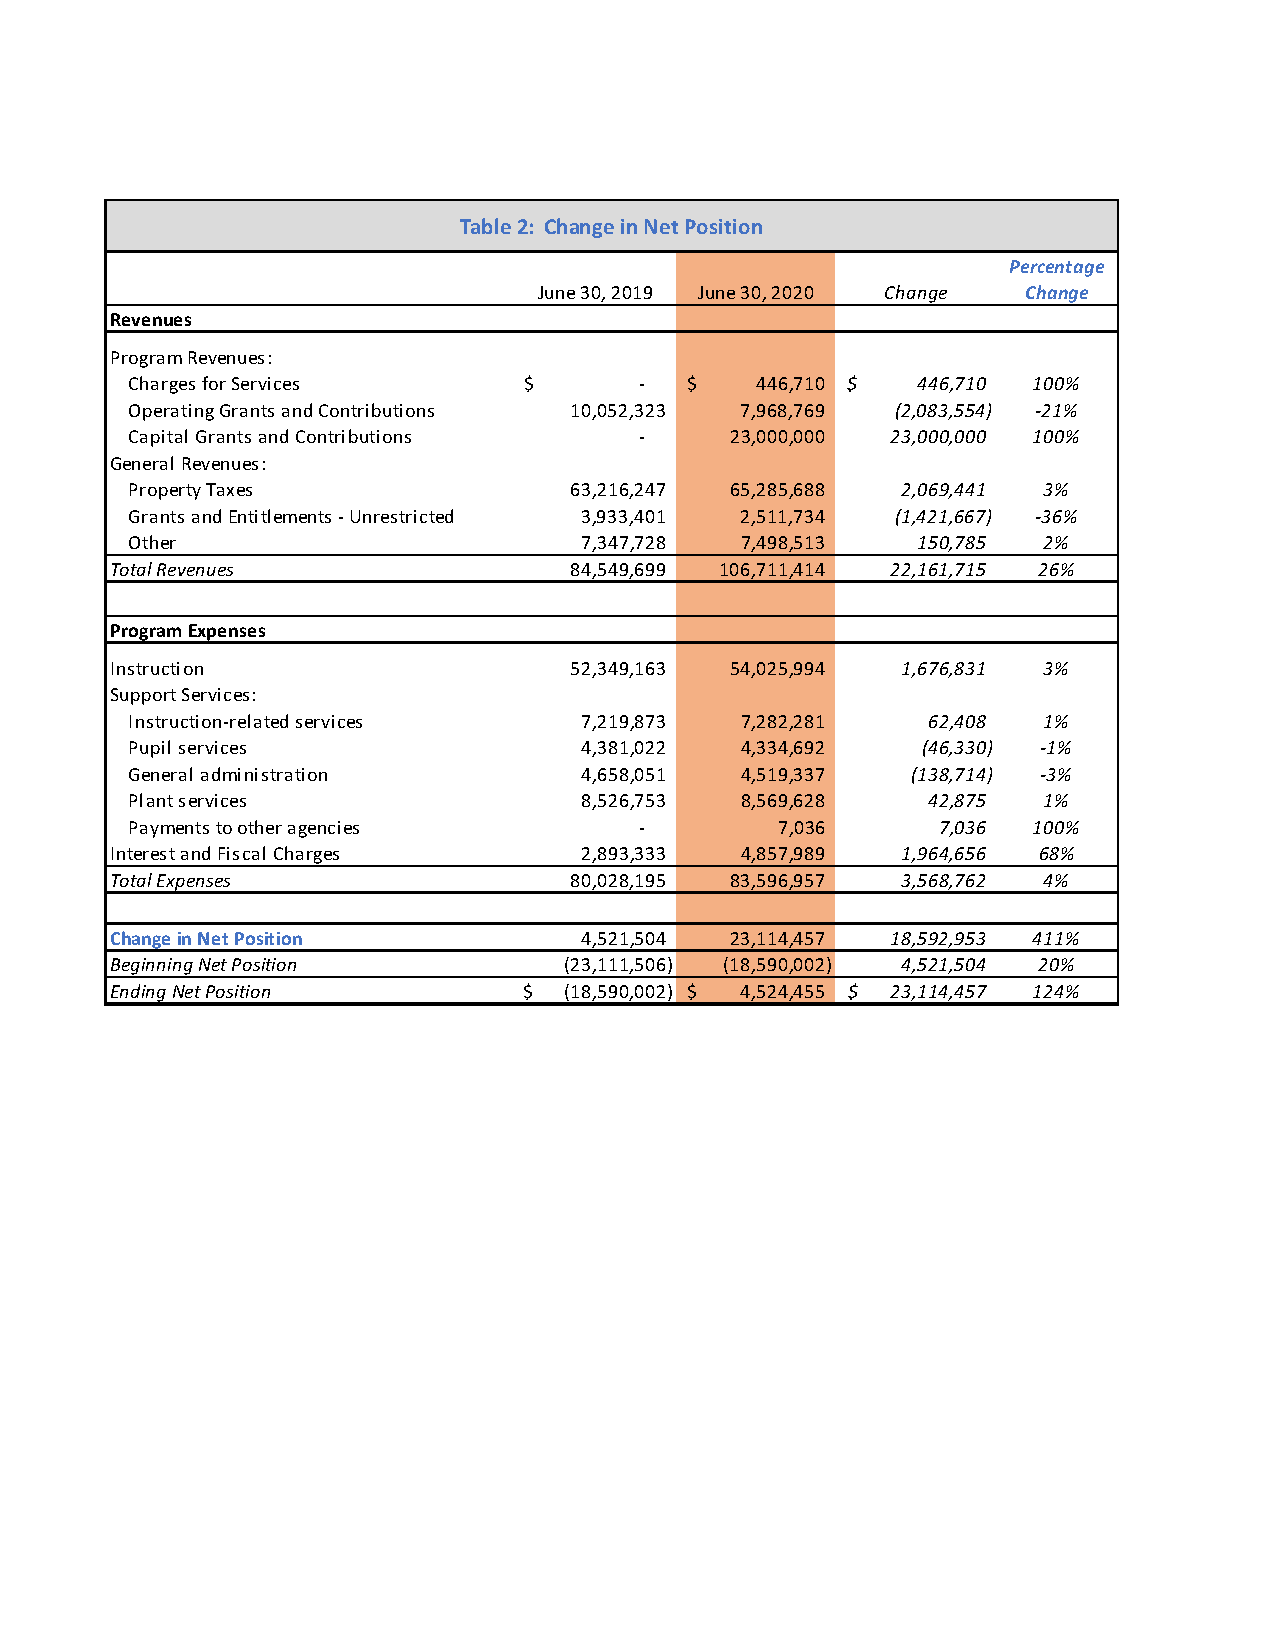
\includegraphics[width=\textwidth]{CAFR-YE2020_Change_in_Net_Position}\\
  \footnotesize\raggedright\textcite[7]{Kenyon2021}.
\end{figure}

\begin{figure}
  \centering
  \caption[LASD YE 2020 Net Cost of Services]{\textit{LASD YE 2020 Net Cost of Services}}\label{fig:Cost_Services}
  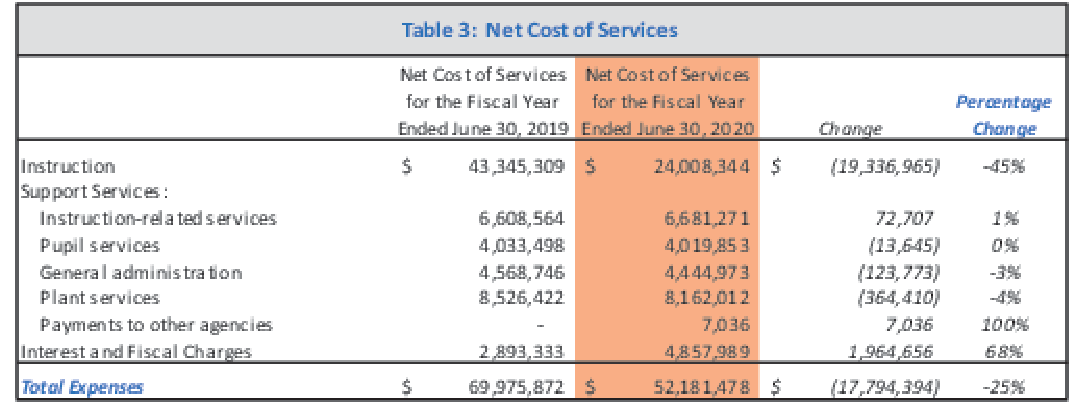
\includegraphics[width=\textwidth]{CAFR-YE2020_Net_Cost_of_Services}\\
  \footnotesize\raggedright\textcite[9]{Kenyon2021}.
\end{figure}

\begin{figure}
  \centering
  \caption[LASD YE 2020 Capital Assets]{\textit{LASD YE 2020 Capital Assets}}\label{fig:Capital_Assets}
  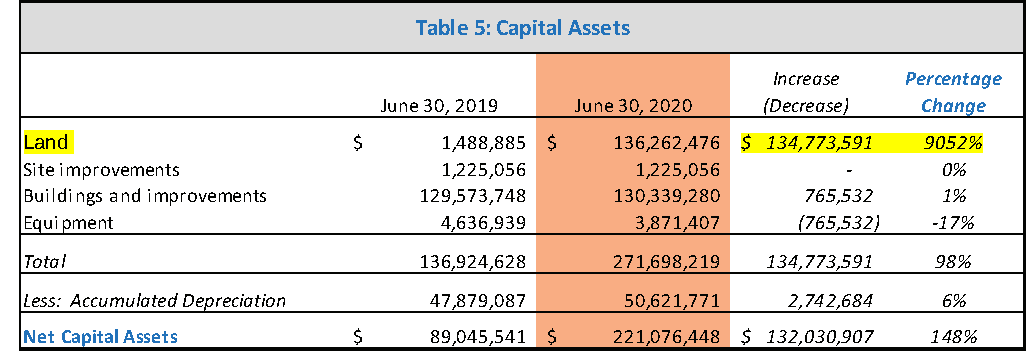
\includegraphics[width=\textwidth]{CAFR-YE2020_Capital_Assets}\\
  \footnotesize\raggedright\textcite[10]{Kenyon2021}.
\end{figure}

\begin{figure}
  \centering
  \caption[LASD YE 2020 Long-term Liabilities]{\textit{LASD YE 2020 Long-term Liabilities}}\label{fig:Long-term_Liabilities}
  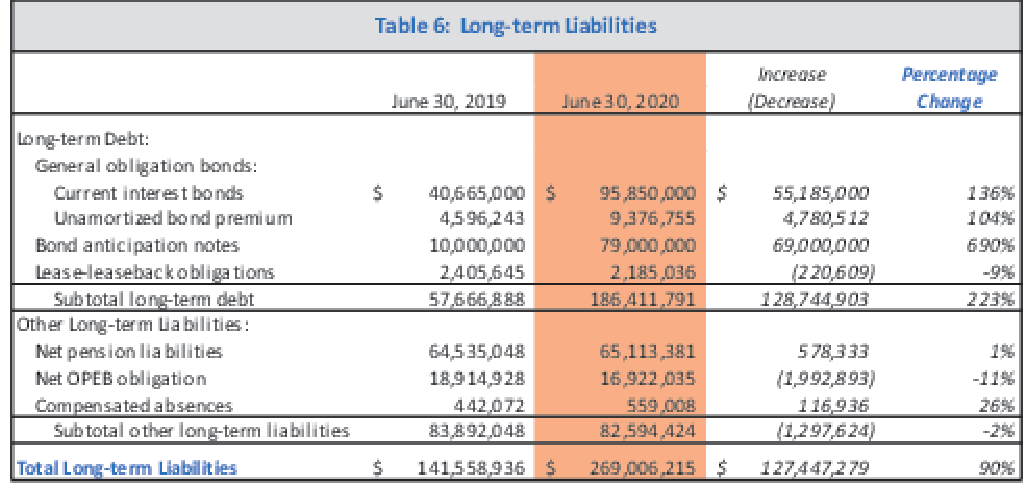
\includegraphics[width=\textwidth]{CAFR-YE2020_Long-term_Liabilities}\\
  \footnotesize\raggedright\textcite[11]{Kenyon2021}.
\end{figure}%

LASD rolls up its detailed financial data into a single multi-year summary, as shown in \prettyref{fig:multi-year-proj}. In addition to purely financial data, the multi-year summary includes the key
assumptions that were behind the numbers. In fact, the first section of Figure~\ref{fig:multi-year-proj} is only assumptions, and it is those assumptions which drive the numbers in Sections 2–4. The value of this summary is that it captures in one table the key data needed to make budgetary decisions and thus might serve as a template for what data is important. 

\begin{figure}[!t]
  \centering
  \caption[LASD 2019–20 Multi-Year Projection]{\textit{LASD 2019–20 Multi-Year Projection}}\label{fig:multi-year-proj}
  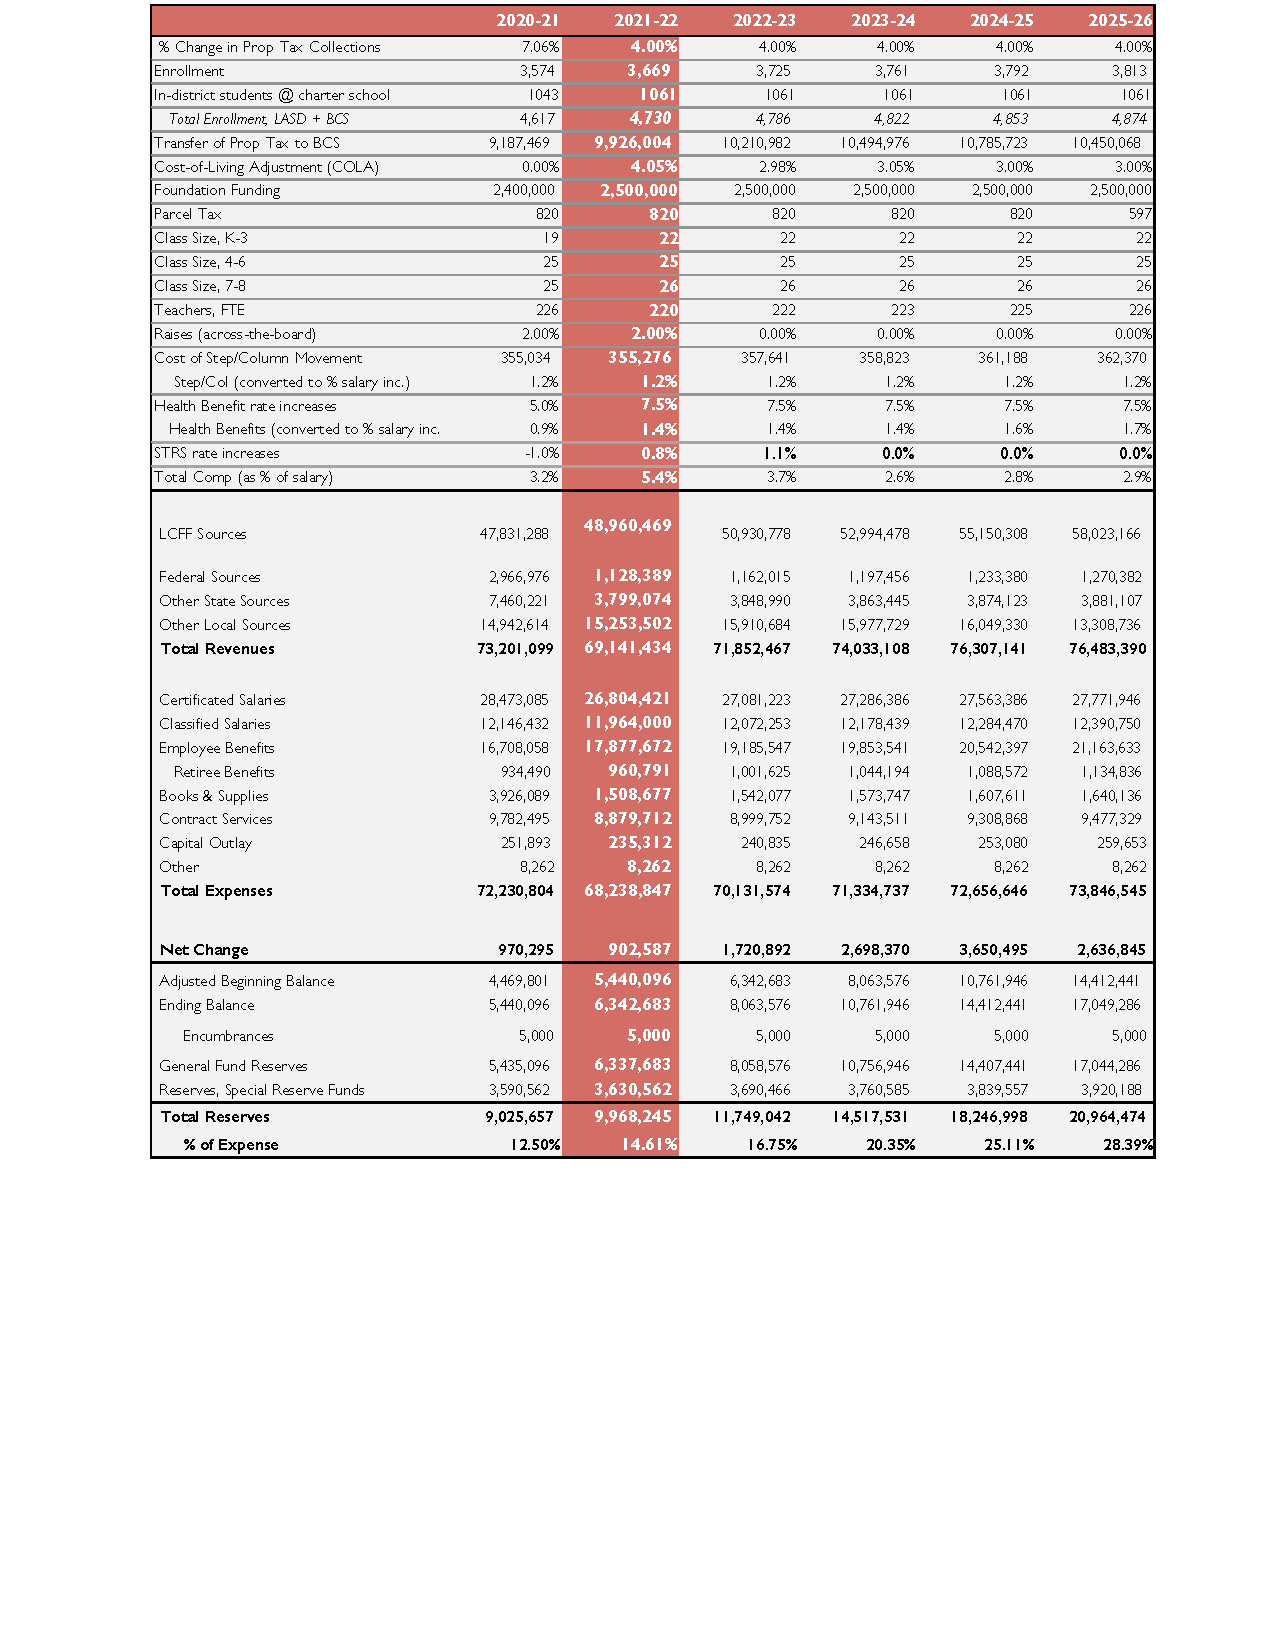
\includegraphics[width=\textwidth]{LASD_Multi_Year_Projection}\
  \footnotesize\raggedright\textcite[137]{Kenyon2021a}.
\end{figure}\bigskip%


%%% Local Variables:
%%% mode: latex
%%% TeX-master: "Rocketship_Education-An_Exploratory_Public_Policy_Case_Study"
%%% End:

\clearforchapter%%% Time-stamp: <2023-05-22 11:01:28 vladimir>
%%% Copyright (C) 2019-2023 Vladimir G. Ivanović
%%% Author: Vladimir G. Ivanović <vladimir@acm.org>
%%% ORCID: https://orcid.org/0000-0002-7802-7970

\chapter{Rocketship Property Information}\label{ch:rocketship-property-info}
\bigskip%
Each of the 10 existing Rocketship schools in Santa Clara County which were listed in \prettyref{tab:RocketshipLocations} are described in a section below. Each section comprises some basic property information, a plat map of the property, its assessed valuation over the last three years, and a satellite photograph of the school site.

Except for the photos, all of the information presented in this appendix is available from the the Office of the Assessor, County of Santa Clara, under the heading ``Real Property Search'' (\url{https://tinyurl.com/assessors-office-santa-clara}).

\begin{footnote}
Note: The earliest date under ``Taxable Amount'' is supposed to be the sale price, but figures from the Office of the Assessor seem to omit recording the sale year and only pick up a year after the sale date.
\end{footnote}

\clearpage

%%%%%%%%%%%%%%%%%%%%%%%%%%%%%%%%%%%%%%%%%%%%%%%%%%%%%%%%%%%%%%%%%%%%%%%%%%%%%%%%%%%%%%%%%%%%%%%%%%%%%%%%%%%%%%%%%%%%%%%%%

\section{Mateo Sheedy}\label{sec:mateo-sheedy-info}
\begin{table}[htb]
  \SingleSpacing%
  \caption[Mateo Sheedy: Property Information]{\textit{Mateo Sheedy: Property Information}}\label{tab:mateo-sheedy-prop-info}
  \begin{tabular}{ll}
    \toprule
    Owner                 & Launchpad Development One, LLC \\
    Property Address      & 788 Locust St., San José, CA 95110 \\
    Assessor's Parcel No. &  264–34–076 \\
    Size (acres)          & 1.55 \\
    Date of Last Sale     & 11 Mar 2016 \\
    \bottomrule
  \end{tabular}
\end{table}

\begin{figure}[hbt]
    \caption[Mateo Sheedy Plat Map]{\textit{Mateo Sheedy Plat Map}}\label{fig:mateo-sheedy-plat-map}
    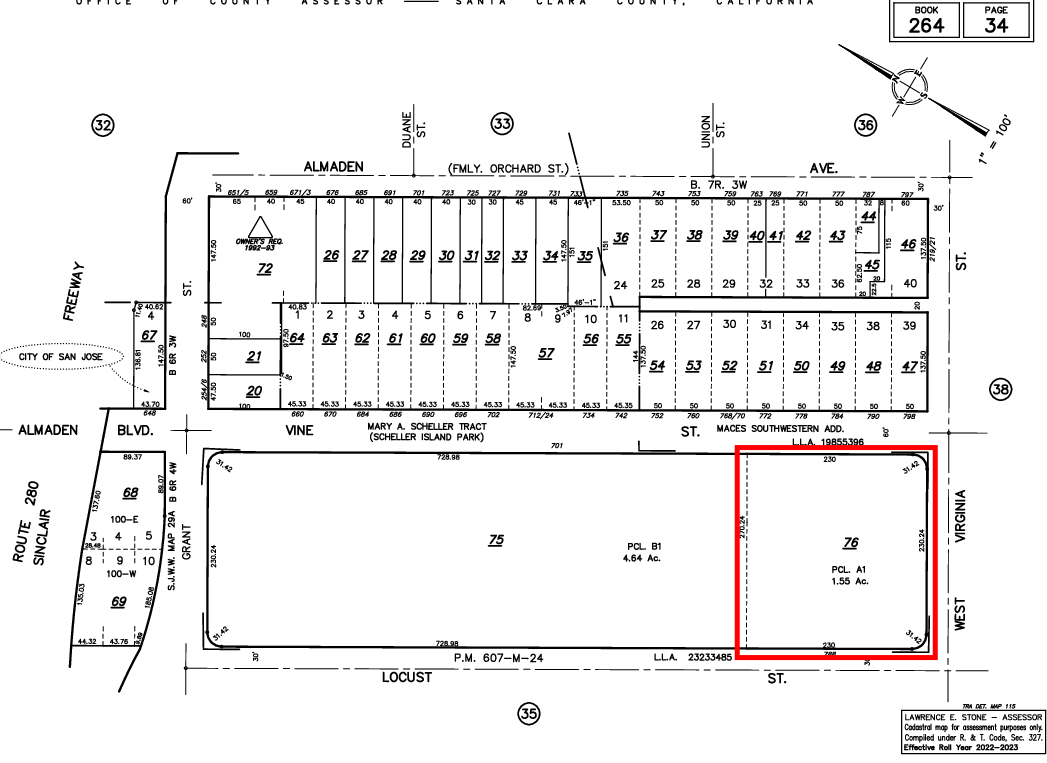
\includegraphics[width=\textwidth]{Assessor-Info/mateo-sheedy-plat-map-264-34}\\ %chktex 8
    \footnotesize{Santa Clara County Assessor's Office (n.d.). [Plat Map]. Retrieved 22 Dec 2022 from  \url{https://tinyurl.com/mateo-sheedy-plat-map}}.
\end{figure}

\begin{table}[hbt]
  \SingleSpacing%
  \caption[Mateo Sheedy: Taxable Amount of Assessed Propery]{\textit{Mateo Sheedy: Taxable Amount of Assessed Property}}\label{tab:mateo-sheedy-taxable-amount}
  \begin{tabular}{llll}
    \toprule
    Year & Land        & Improvements & Total Assessed Value \\
    \midrule
    2022 & \$3,011,899 & \$780,861    & \$3,792,760 \\
    2021 & \$2,952,843 & \$765,550    & \$3,718,550 \\
    2020 & \$2,922,566 & \$757,701    & \$3,680,267 \\
    2019 & \$2,865,261 & \$742,845    & \$3,608,106 \\
    2018 & \$2,809,080 & \$728,280    & \$3,537,360 \\
    2017 & \$2,754,000 & \$714,000    & \$3,468,000 \\
    \bottomrule
  \end{tabular}
\end{table}

\begin{figure}[hbt]
  \caption[Mateo Sheedy Satellite Photo]{\textit{Mateo Sheedy Satellite Photo}}\label{fig:mateo-sheedy-sat-photo}
  \includegraphics[width=\textwidth]{Satellite-Photos/mateo-sheedy-sat-photo}\\ %chktex 8
  \footnotesize{Google. (n.d). [Google Earth image]. Retrieved 19 Dec 2022 from \url{https://tinyurl.com/mateo-sheedy}.}
\end{figure}

%%%%%%%%%%%%%%%%%%%%%%%%%%%%%%%%%%%%%%%%%%%%%%%%%%%%%%%%%%%%%%%%%%%%%%%%%%%%%%%%%%%%%%%%%%%%%%%%%%%%%%%%%%%%%%%%%%%%%%%%%

\clearpage
\section{Sí Si Puede}\label{sec:sí-si-puede-info}
\begin{table}[htb]
  \SingleSpacing%
  \caption[Sí Si Puede: Property Information]{\textit{Sí Si Puede: Property Information}}\label{tab:sí-si-puede-prop-info}
  \begin{tabular}{ll}
    \toprule
    Owner (starting 20 Mar 2009) & Rocketship Dobern Property, LLC \\
    Owner (starting 20 Mar 2014) & Launchpad Development Two, LLC \\
    Property Address      & 2249 Dobern Ave, San José, CA 95116 \\
    Assessor's Parcel No. &  481–32–059 \\
    Size (acres)          &  1.668\\
    Date of First Sale    &  20 Mar 2009 \\
    Date of Last Sale     &  20 Mar 2014 \\
    \bottomrule
  \end{tabular}
\end{table}

\begin{figure}[hbt]
  \centering
  \caption[śi si puede plat map]{\textit{Śi si puede plat map}}\label{fig:śi-si-puede-plat-map}
  \noindent\includegraphics[width=\textwidth]{Assessor-Info/śi-si-puede-plat-map-481-32}\\ %chktex 8
  \footnotesize{Santa Clara County Assessor's Office (n.d.). [Plat Map]. Retrieved 22 Dec 2022, from \url{https://tinyurl.com/si-si-puede-plat-map}}.
\end{figure}

\begin{table}[htb]
  \SingleSpacing%
  \caption[Sí Si Puede: Taxable Amount of Assessed Propery]{\textit{Sí Si Puede: Taxable Amount of Assessed Property}}\label{tab:sí-si-puede-taxable-amount}
  \begin{tabular}{llll}
    \toprule
    Year & Land        & Improvements & Total Assessed Value \\
    \midrule
    2022 & \$5,545,914 & \$5,411,914  & \$10,957,828 \\
    2021 & \$5,437,171 & \$5,305,799  & \$10,742,970 \\
    2020 & \$5,381,420 & \$5,251,395  & \$10,632,815 \\
    \ldots \\
    2014 & \$1,932,914 & \$5,534,530  & \$7,467,444 \\
    \ldots \\
    2010 & \$1,835,639 & \$5,256,000  & \$7,091,639 \\
    \bottomrule
  \end{tabular}
\end{table}

\begin{figure}[hbt]
  \centering
  \caption[Sí Si Puede Satellite Photo]{\textit{Sí Si Puede Satellite Photo}}\label{fig:sí-si-puede-sat-photo}
  \includegraphics[height=0.667\textheight]{Satellite-Photos/sí-si-puede-sat-photo}\\ %chktex 8
  \footnotesize
  Google. (n.d). [Google Earth image]. Retrieved 19 Dec 2022, from \url{https://tinyurl.com/si-si-puede-v2} %chktex 1
\end{figure}

%%%%%%%%%%%%%%%%%%%%%%%%%%%%%%%%%%%%%%%%%%%%%%%%%%%%%%%%%%%%%%%%%%%%%%%%%%%%%%%%%%%%%%%%%%%%%%%%%%%%%%%%%%%%%%%%%%%%%%%%%

\clearpage
\section{Los Sueños}\label{sec:los-suenos-info}
\begin{table}[htb]
  \SingleSpacing%
  \caption[Los Sueños: Property Information]{\textit{Los Sueños: Property Information}}\label{tab:los-sueños-prop-info}
  \begin{tabular}{ll}
    \toprule
    Owner                  & Launchpad Development Three, LLC \\
    Property Address       & 331 S. 34th St, San José, CA 95116 \\
    Assessor's Parcel Nos. & \multirow[t]{2}{1in}{481–45–001 481–45–039} \\
    \\
    Size (acres)           & 0.482 + 0.449 = 0.93 \\
    Date of Last Sale      & 19 Apr 2010 \\
    \bottomrule
  \end{tabular}
\end{table}

\begin{figure}[hbt]
  \caption[Los Sueños Plat Map]{\textit{Los Sueños Plat Map}}\label{fig:los-sueños-plat-map}
  \includegraphics[width=\textwidth]{Assessor-Info/los-sueños-plat-map-481-45}\\ %chktex 8
  \footnotesize{Santa Clara County Assessor's Office (n.d.). [Plat Map]. Retrieved 23 Dec 2022 from  \url{https://tinyurl.com/los-suenos-plat-map}}.
\end{figure}

\begin{table}[hbt]
  \SingleSpacing%
  \caption[Los Sueños: Taxable Amount of Assessed Propery]{\textit{Los Sueños: Taxable Amount of Assessed Property}}\label{tab:los-sueños-taxable-amount}
  \begin{tabular}{llll}
    \toprule
    Year & Land      & Improvements & Total Assessed Value \\
    \midrule
    2022 & \$486,545 & \$6,510,874  & \$6,997,419 \\
    2021 & \$477,005 & \$6,383,210  & \$6,860,215 \\
    2020 & \$472,114 & \$6,317,759  & \$6,789,873 \\
    \ldots \\
    2011 & \$906,852 &\$5,393,000   & \$6,299,788 \\
    \bottomrule
  \end{tabular}
\end{table}

\begin{figure}[hbt]
  \caption[Los Sueños Satellite Photo]{\textit{Los Sueños Satellite Photo}}\label{fig:los-sueños-sat-photo}
  \includegraphics[width=\textwidth]{Satellite-Photos/los-sueños-sat-photo}\\ %chktex 8
  \footnotesize{Google. (n.d). [Google Earth image]. Retrieved 23 Dec 2022 from \url{https://tinyurl.com/los-suenos-v4}.}
\end{figure}

%%%%%%%%%%%%%%%%%%%%%%%%%%%%%%%%%%%%%%%%%%%%%%%%%%%%%%%%%%%%%%%%%%%%%%%%%%%%%%%%%%%%%%%%%%%%%%%%%%%%%%%%%%%%%%%%%%%%%%%%%

\clearpage
\section{Discovery Prep}\label{sec:discover-prep-info}
\begin{table}[htb]
  \SingleSpacing%
  \caption[Discovery Prep: Property Information]{\textit{Discovery Prep: Property Information}}\label{tab:discovery-prep-prop-info}
  \begin{tabular}{ll}
    \toprule
    Owner                 & Launchpad Development Five, LLC \\
    Property Address      & 370 Wooster Ave, San José, CA 95116 \\
    Assessor's Parcel No. &  249–65–079 \\
    Size (acres)          & 1.652 \\
    Date of Last Sale     & 30 Mar 2011\\
    \bottomrule
  \end{tabular}
\end{table}

\begin{figure}[hbt]
    \caption[Discovery Prep Plat Map]{\textit{Discovery Prep Plat Map}}\label{fig:discovery-prep-plat-map}
    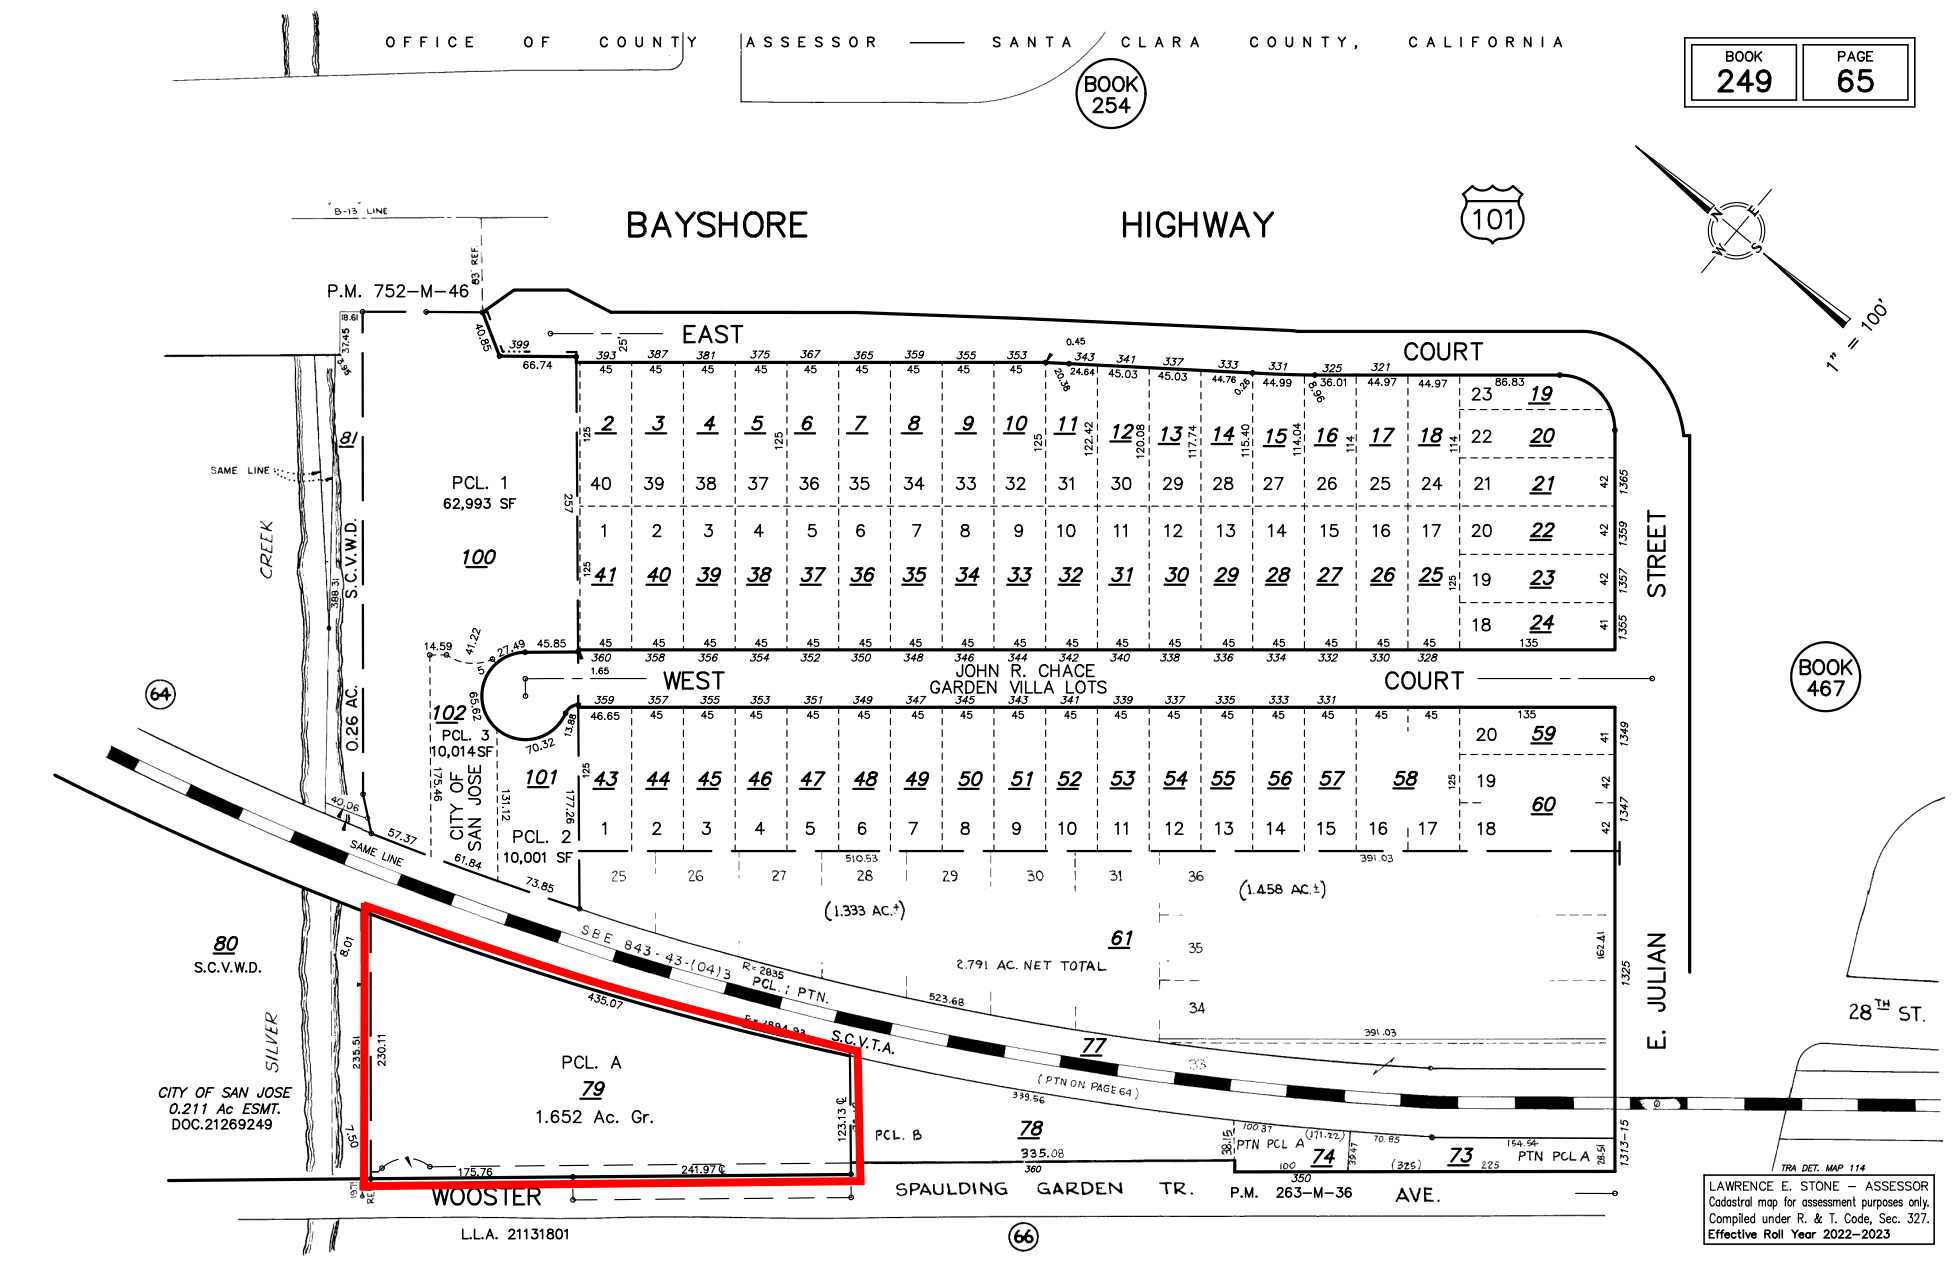
\includegraphics[width=\textwidth]{Assessor-Info/discovery-prep-plat-map-249-65}\\ %chktex 8
    \footnotesize{Santa Clara County Assessor's Office (n.d.). [Plat Map]. Retrieved 23 Dec 2022 from  \url{https://tinyurl.com/discovery-prep-plat-map}}.
\end{figure}

\begin{table}[hbt]
  \SingleSpacing%
  \caption[Discovery Prep: Taxable Amount of Assessed Propery]{\textit{Discovery Prep: Taxable Amount of Assessed Property}}\label{tab:discovery-prep-taxable-amount}
  \begin{tabular}{llll}
    \toprule
    Year & Land        & Improvements & Total Assessed Value \\
    \midrule
    2022 & \$2,414,563 & \$4,289,318  & \$6,703,881 \\
    2021 & \$2,367,219 & \$4,205,214  & \$6,572,433 \\
    2020 & \$2,342,947 & \$4,162,095  & \$6,505,042 \\
    \ldots \\
    2012 & \$2,040,000 & \$3,623,930  & \$5,664,930 \\
    \bottomrule
  \end{tabular}
\end{table}

\begin{figure}[hbt]
  \caption[Discovery Prep Satellite Photo]{\textit{Discovery Prep Satellite Photo}}\label{fig:discovery-prep-sat-photo}
  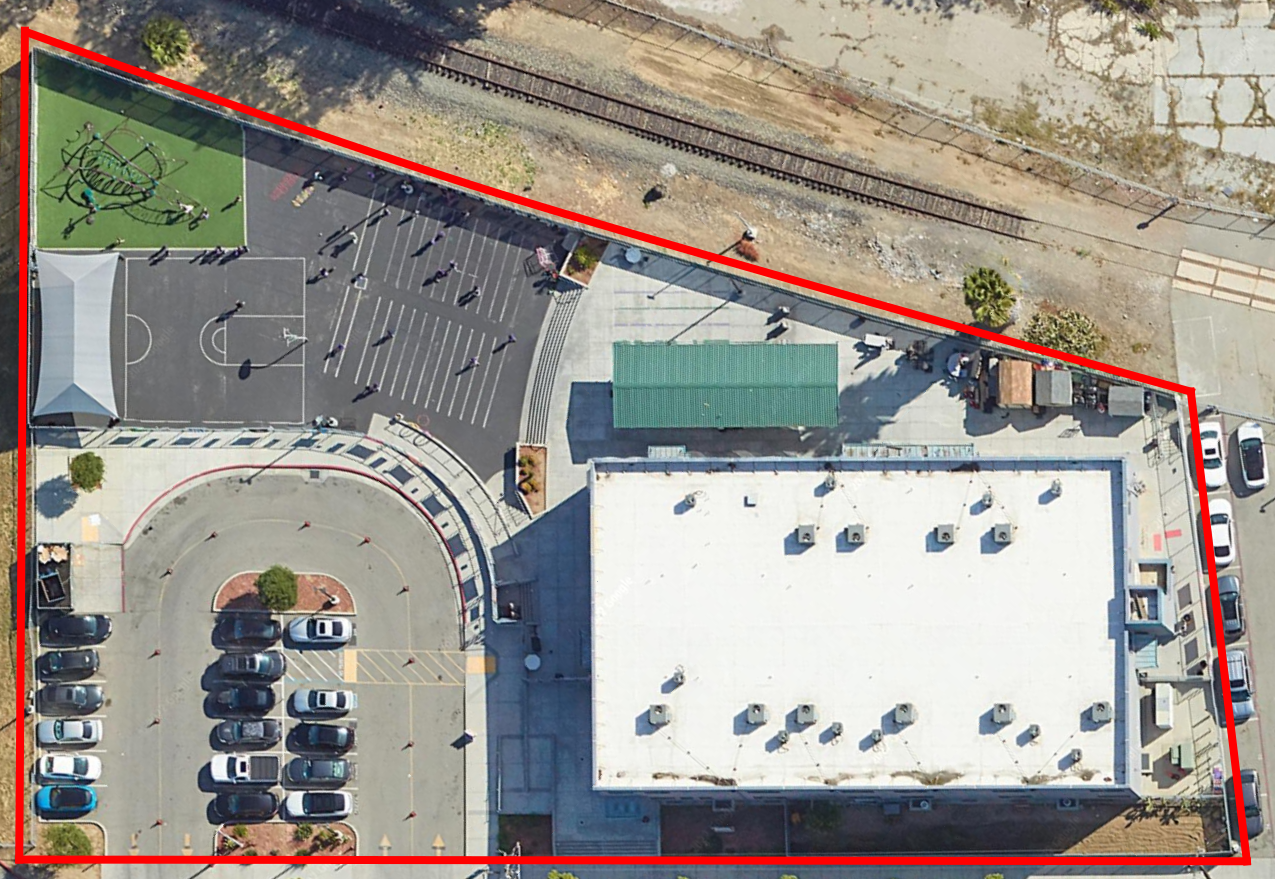
\includegraphics[width=\textwidth]{Satellite-Photos/discovery-prep-sat-photo}\\ %chktex 8
  \footnotesize{Google. (n.d). [Google Earth image]. Retrieved 23 Dec 2022 from \url{https://tinyurl.com/discovery-prep-v2}.}
\end{figure}

%%%%%%%%%%%%%%%%%%%%%%%%%%%%%%%%%%%%%%%%%%%%%%%%%%%%%%%%%%%%%%%%%%%%%%%%%%%%%%%%%%%%%%%%%%%%%%%%%%%%%%%%%%%%%%%%%%%%%%%%%

\clearpage
\section{Mosaic}\label{sec:mosaic-info}
\begin{table}[htb]
  \SingleSpacing%
  \caption[Mosaic: Property Information]{\textit{Mosaic: Property Information}}\label{tab:mosaic-prop-info}
  \begin{tabular}{ll}
    \toprule
    Property Address      & 950 Owsley Ave, San José, CA 95122 \\
    Assessor's Parcel No. & 477–34–088 \\
    Size                  & 1.011ac \\
    Date of Last Sale     & 24 May 2011 \\
    \bottomrule
  \end{tabular}
\end{table}

\begin{figure}[hbt]
    \caption[Mosaic Plat Map]{\textit{Mosaic Plat Map}}\label{fig:mosaic-plat-map}
    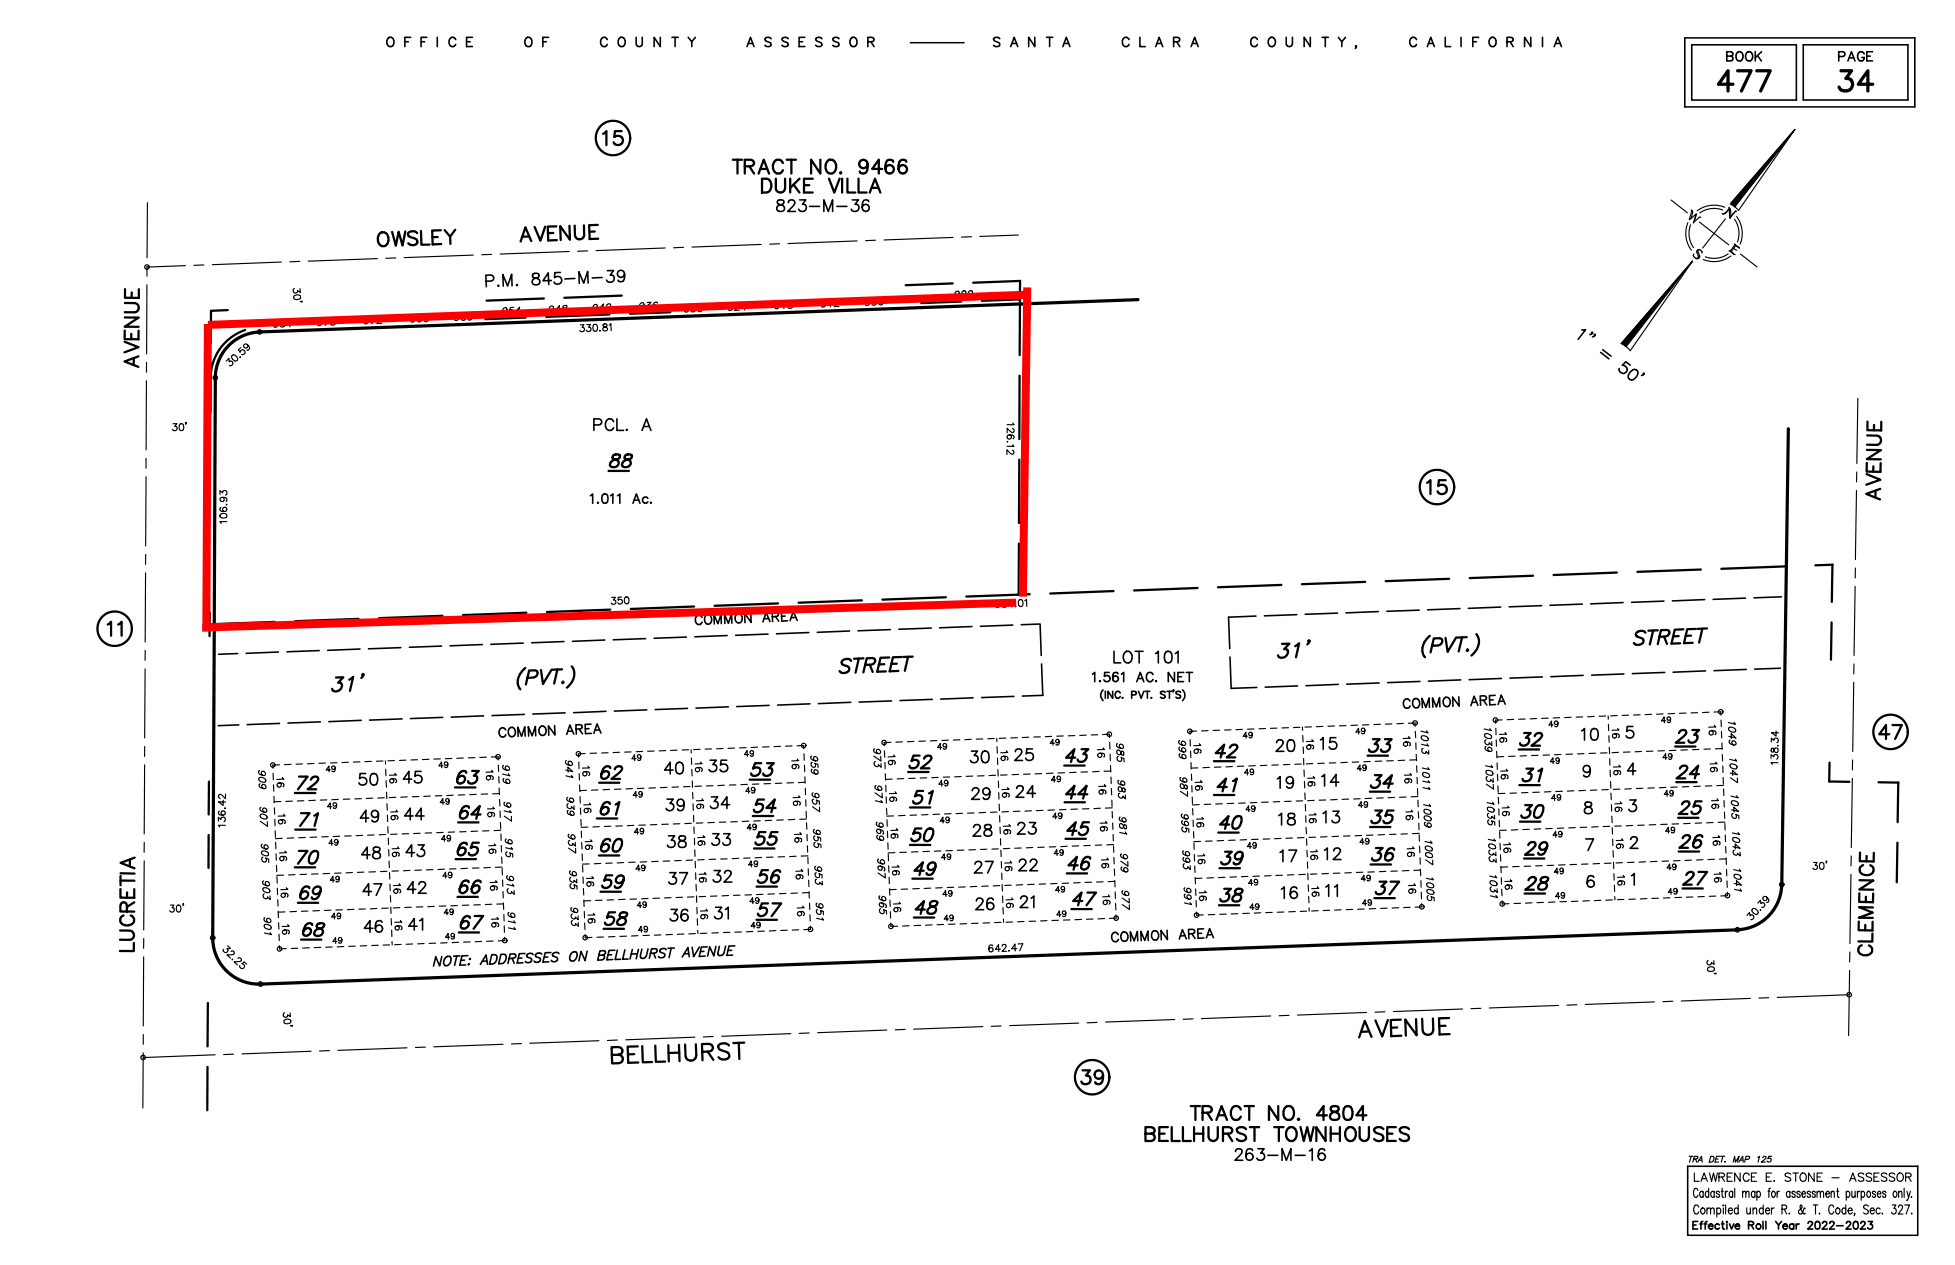
\includegraphics[width=\textwidth]{Assessor-Info/mosaic-plat-map-477-34}\\ %chktex 8
    \footnotesize{Santa Clara County Assessor's Office (n.d.). [Plat Map]. Retrieved 23 Dec 2022 from  \url{https://tinyurl.com/mosaic-plat-map}}.
\end{figure}

\begin{table}[hbt]
  \SingleSpacing%
  \caption[Mosaic: Taxable Amount of Assessed Propery]{\textit{Mosaic: Taxable Amount of Assessed Property}}\label{tab:mosaic-taxable-amount}
  \begin{tabular}{llll}
    \toprule
    Year & Land        & Improvements & Total Assessed Value \\
    \midrule
    2022 & \$1,851,242 & \$4,971,161 & \$6,822,403 \\
    2021 & \$1,814,944 & \$4,873,688 & \$6,688,632 \\
    2020 & \$1,796,334 & \$4,823,715 & \$6,620,049 \\
    \bottomrule
  \end{tabular}
\end{table}

\begin{figure}[hbt]
  \caption[Mosaic Satellite Photo]{\textit{Mosaic Satellite Photo}}\label{fig:mosaic-sat-photo}
  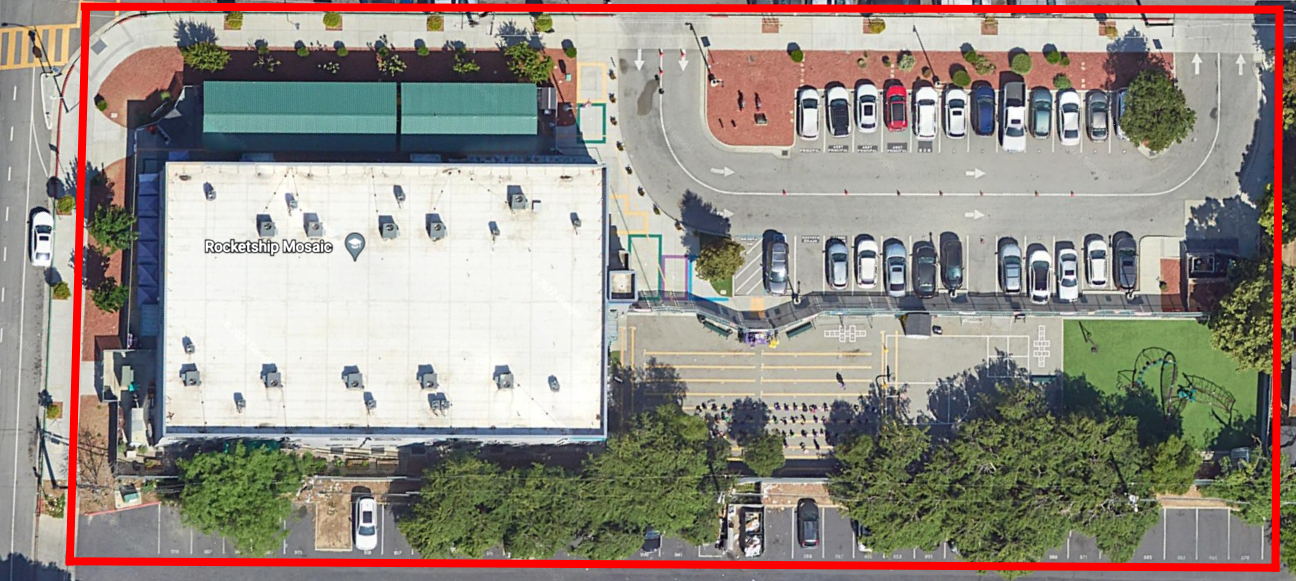
\includegraphics[width=\textwidth]{Satellite-Photos/mosaic-sat-photo}\\ %chktex 8
  \footnotesize{Google. (n.d). [Google Earth image]. Retrieved 23 Dec 2022 from \url{https://tinyurl.com/mosaic-v3}.}
\end{figure}

%%%%%%%%%%%%%%%%%%%%%%%%%%%%%%%%%%%%%%%%%%%%%%%%%%%%%%%%%%%%%%%%%%%%%%%%%%%%%%%%%%%%%%%%%%%%%%%%%%%%%%%%%%%%%%%%%%%%%%%%%

\clearpage
\section{Brilliant Minds}\label{sec:brilliant-minds-info}

\begin{table}[htb]
  \SingleSpacing%
  \caption[Brilliant Minds: Property Information]{\textit{Brilliant Minds: Property Information}}\label{tab:brilliant-minds-prop-info}
  \begin{tabular}{ll}
    \toprule
    Property Address      & \multirow[t]{2}{3in}{2960 Story Rd, San Jose, CA 95127 \\
    2962 Story Rd, San Jose, CA 95127} \\\\
    Assessor's Parcel No. & 488-03-003 \\
    Size                  & 1.223ac \\
    Date of Last Sale     & 11 Feb 2014\\
    \bottomrule
  \end{tabular}\\\newline
  \noindent\footnotesize{Note: Brilliant Minds occupies a single parcel, along with two churches. It appears to have its own buildings, but shares the single parking lot. The size of the parcel is 2.446ac, and arbitrarily, half has been allocated to Rocketship Brilliant Minds.}  
\end{table}


\begin{figure}[t]
  \centering
  \caption[Brilliant Minds Plat Map]{\textit{Brilliant Minds Plat Map}}\label{fig:brilliant-minds-plat-map}
  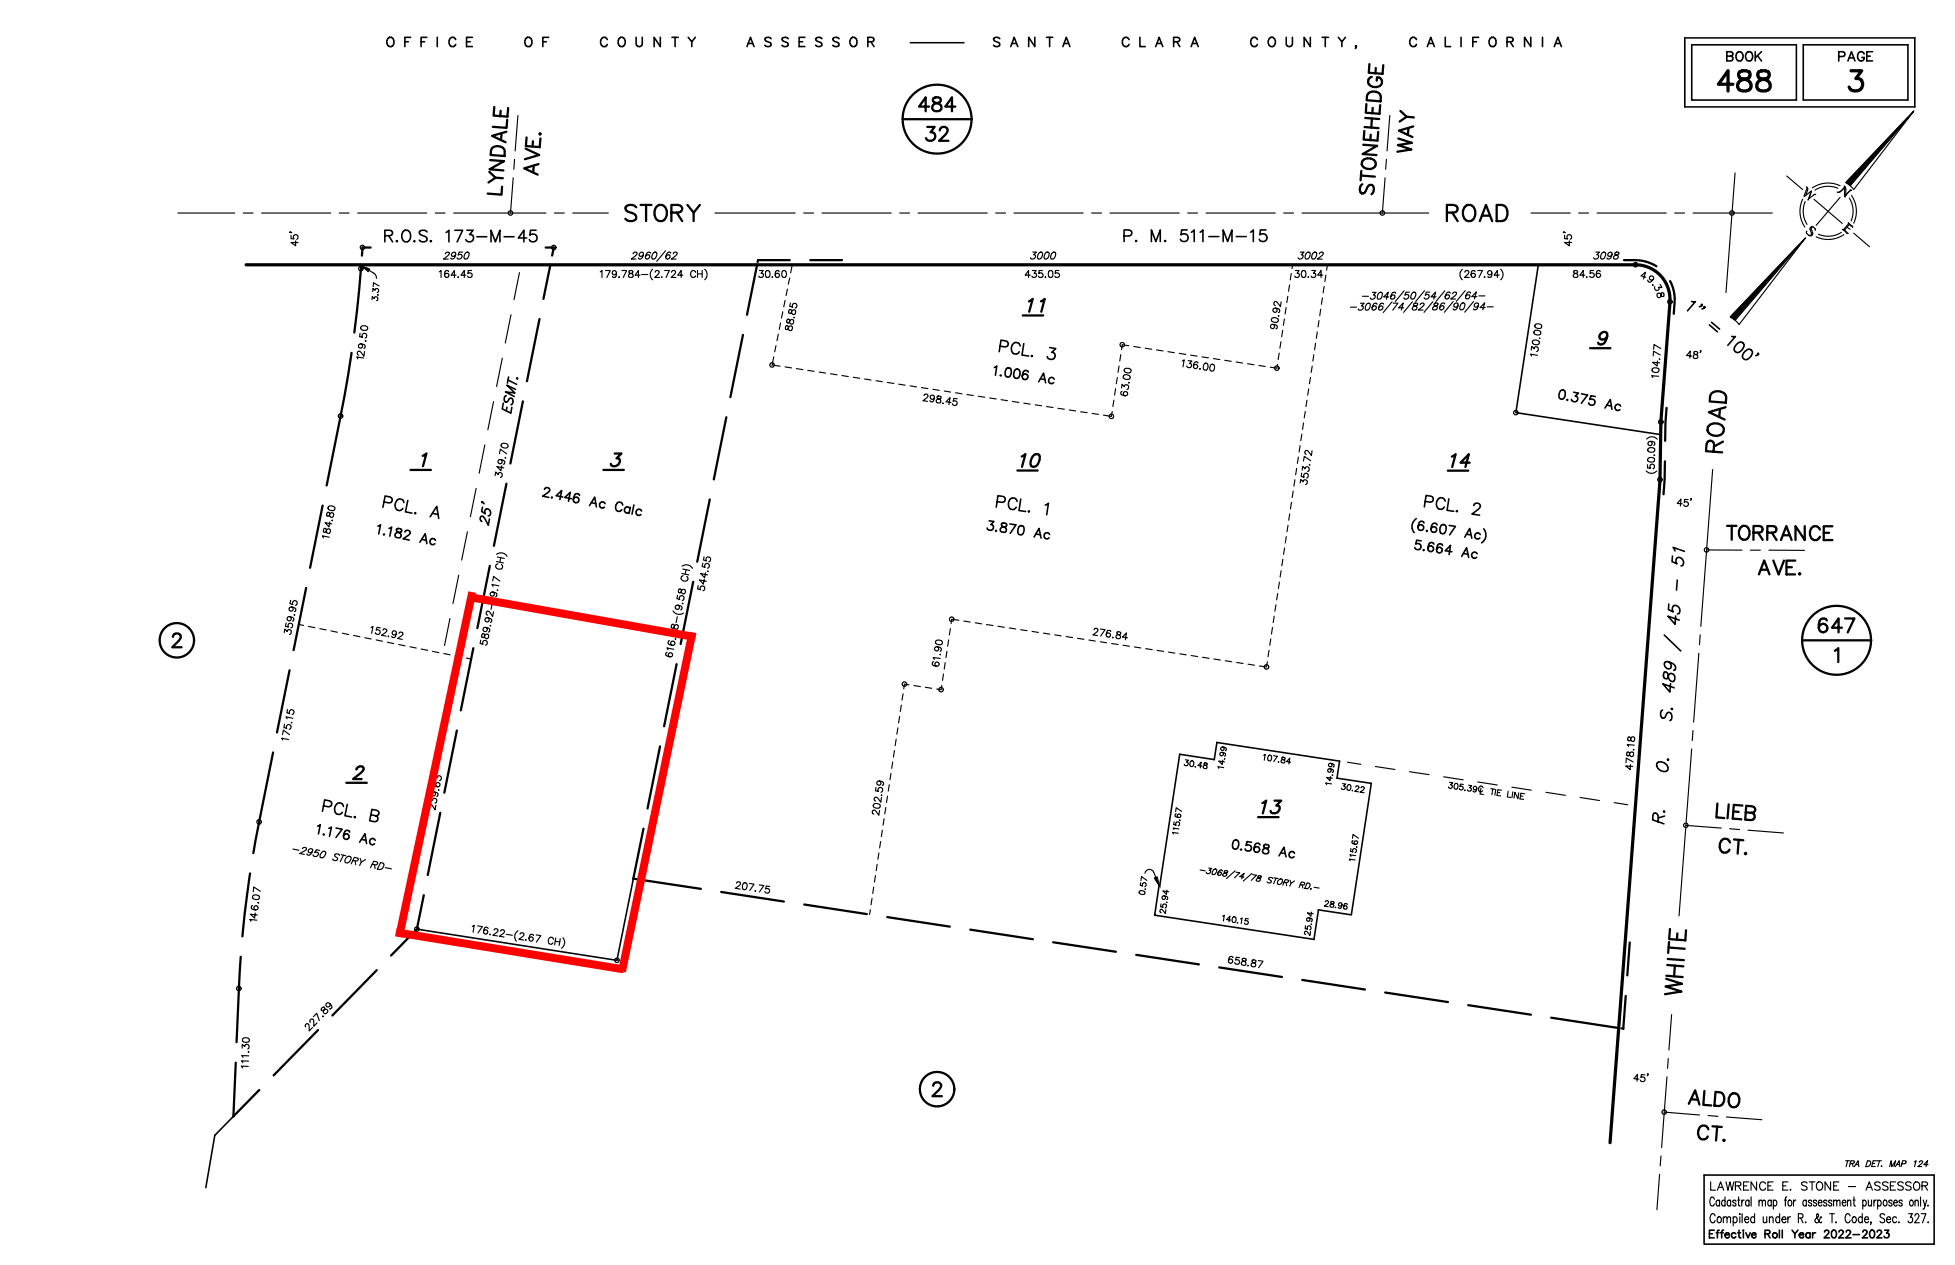
\includegraphics[width=\textwidth]{Assessor-Info/brilliant-minds-plat-map-488-03}\\ %chktex 8
  \footnotesize{Santa Clara County Assessor's Office (n.d.). [Plat Map]. Retrieved 23 Dec 2022 from  \url{https://tinyurl.com/brilliant-minds-plat-map}}.
\end{figure}

\begin{table}[hbt]
\SingleSpacing%
  \caption[Brilliant Minds: Taxable Amount of Assessed Propery]{\textit{Brilliant Minds: Taxablekk Amount of Assessed Property}}\label{tab:brilliant-minds-taxable-amount}
  \begin{tabular}{llll}
    \toprule
   Year  & Land        & Improvements & Total Assessed Value \\
    \midrule
    2022 & \$8,630,187 & \$4,218,635  & \$12,848,822 \\
    2021 & \$8,460,968 & \$4,135,917  & \$12,596,885 \\
    2020 & \$8,374,212 & \$4,093,509  & \$12,467,721 \\
    \bottomrule
  \end{tabular}
\end{table}

\begin{figure}[hbt]
  \centering
  \caption[Brilliant Minds Satellite Photo]{\textit{Brilliant Minds Satellite Photo}}\label{fig:brilliant-minds-sat-photo}
  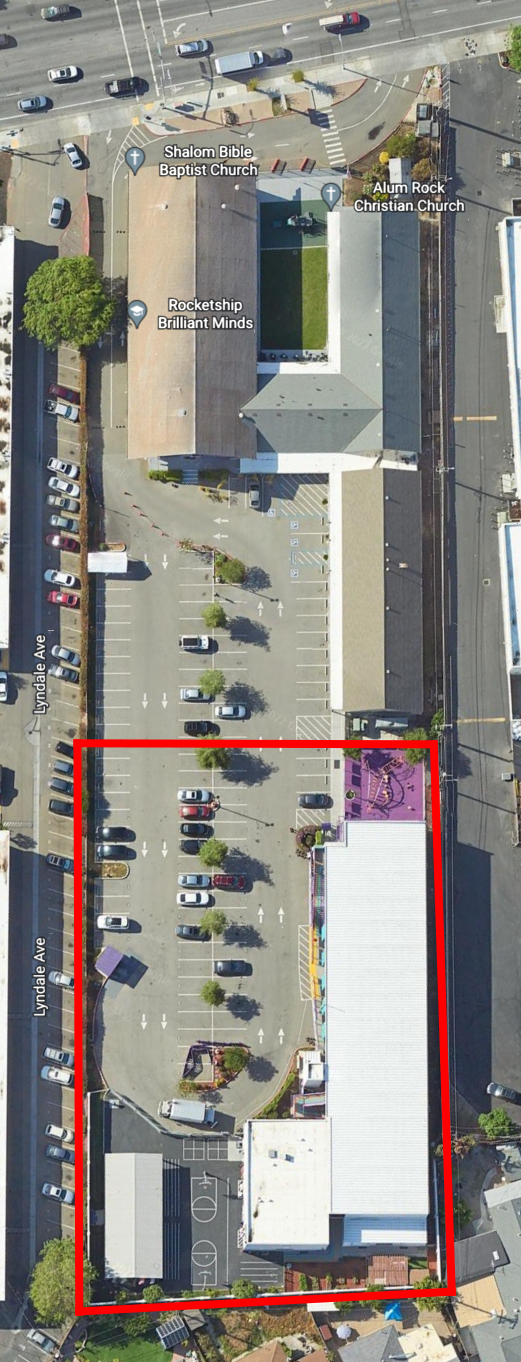
\includegraphics[height=0.9\textheight]{Satellite-Photos/brilliant-minds-sat-photo}\\ %chktex 8
  \footnotesize{Google. (n.d). [Google Earth image]. Retrieved 23 Dec 2022 from \url{https://tinyurl.com/brilliant-minds-v2}.}
\end{figure}

%%%%%%%%%%%%%%%%%%%%%%%%%%%%%%%%%%%%%%%%%%%%%%%%%%%%%%%%%%%%%%%%%%%%%%%%%%%%%%%%%%%%%%%%%%%%%%%%%%%%%%%%%%%%%%%%%%%%%%%%%

\clearpage
\section{Alma Academy}\label{sec:alma-academy-info}
\begin{table}[htb]
  \SingleSpacing%
  \caption[Alma Academy: Property Information]{\textit{Alma Academy}: Property Information}\label{tab:alma-academy-prop-info}
  \begin{tabular}{ll}
    \toprule
    Property Address      & 198 West Alma Ave, San José, CA 95110 \\
    Assessor's Parcel No. & 434–22–{097,098,099,100,119,132} \\
    Size                  & 0.551ac \\
    Date of Last Sale     & 12 Apr 2012 \\
    \bottomrule
  \end{tabular}
\end{table}

\begin{figure}[hbt]
    \caption[Alma Academy Plat Map]{\textit{Alma Academy Plat Map}}\label{fig:alma-academy-plat-map}
    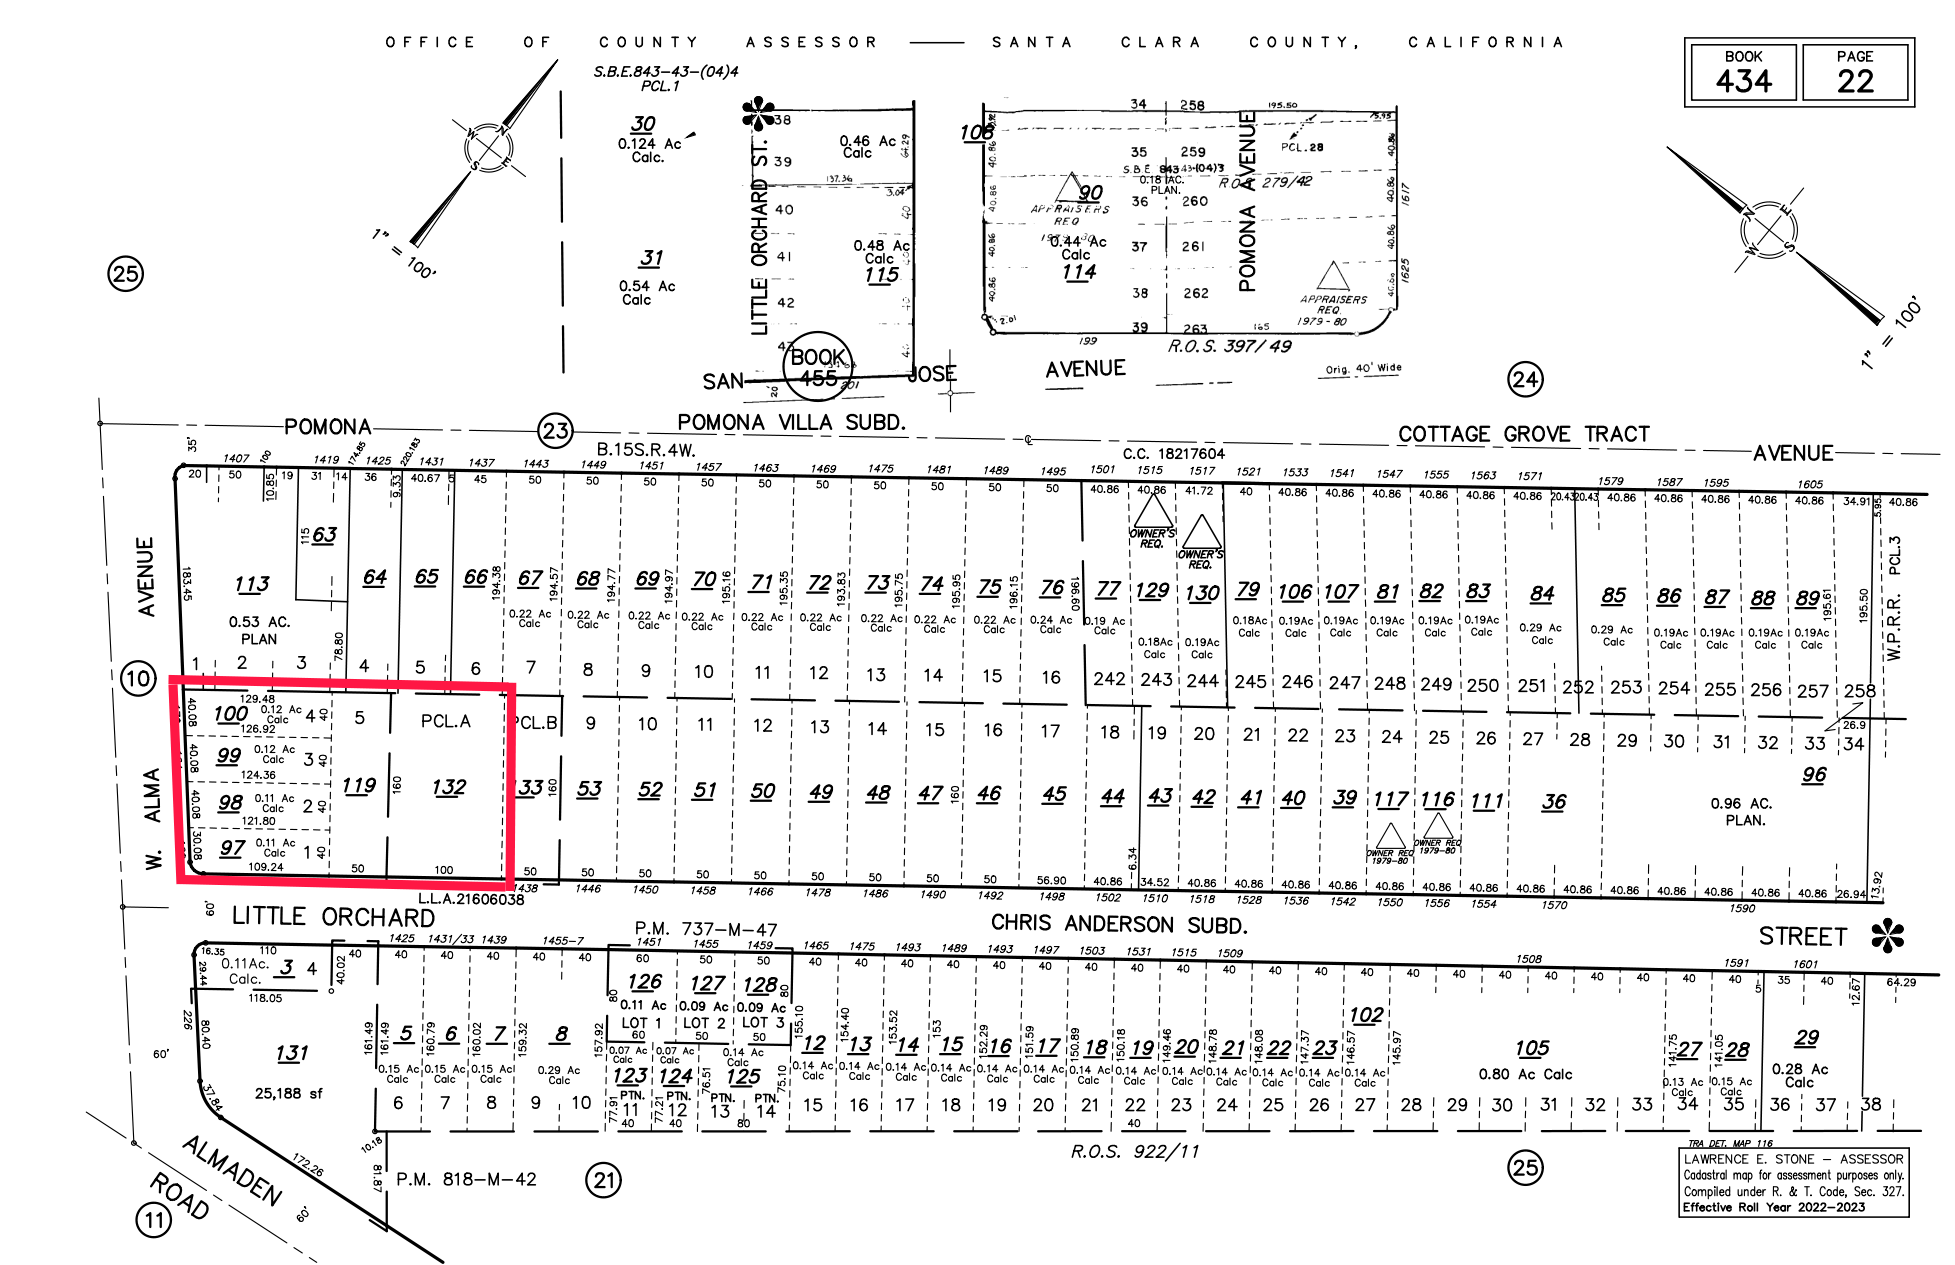
\includegraphics[width=0.9\textwidth]{Assessor-Info/alma-academy-plat-map-434-22}\\ %chktex 8
    \footnotesize{Santa Clara County Assessor's Office (n.d.). [Plat Map]. Retrieved 03 Jan 2023 from  \url{https://tinyurl.com/alma-academy-plat-map-v2}.}
\end{figure}

\begin{table}[hbt]
  \SingleSpacing%
  \caption[Alma Academy: Taxable Amount of Assessed Propery]{\textit{Alma Academy: Taxable Amount of Assessed Property}}\label{tab:alma-academy-taxable-amount}
  \begin{tabular}{llll}
    \toprule
    Year & Land        & Improvements & Total Assessed Value \\
    \midrule
    2022 & \$1,615,598 & \$0          & \$1,615,598 \\
    2021 & \$1,583,932 & \$0          & \$1,583,932 \\
    2020 & \$1,567,686 & \$0          & \$1,567,686 \\
    \bottomrule
  \end{tabular}\\\newline
  \noindent\footnotesize{Note: Rocketship Alma Academy comprises adjacent six parcels, so the assessed value indicated in this table is the sum of all six parcels.}
\end{table}

\begin{figure}[hbt]
  \centering
  \caption[Alma Academy Satellite Photo]{\textit{Alma Academy Satellite Photo}}\label{fig:alma-academy-sat-photo}
  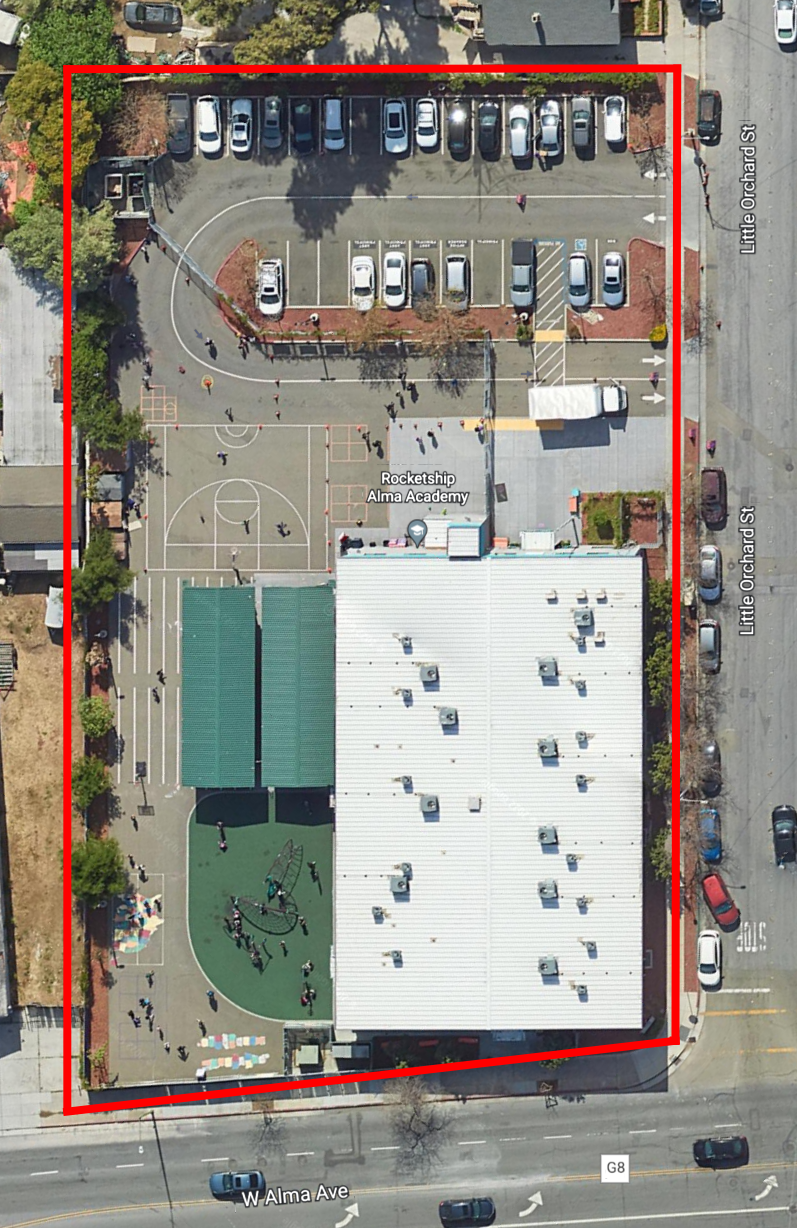
\includegraphics[height=0.667\textheight]{Satellite-Photos/alma-academy-sat-photo}\\ %chktex 8
  \footnotesize{Google. (n.d). [Google Earth image]. Retrieved 03 Jan 2023 from \url{https://tinyurl.com/alma-academy}.}
\end{figure}

%%%%%%%%%%%%%%%%%%%%%%%%%%%%%%%%%%%%%%%%%%%%%%%%%%%%%%%%%%%%%%%%%%%%%%%%%%%%%%%%%%%%%%%%%%%%%%%%%%%%%%%%%%%%%%%%%%%%%%%%%

\clearpage
\section{Spark Academy}\label{sec:spark-academy-info}

\begin{table}[htb]
  \SingleSpacing%
  \caption[Spark Academy: Property Information]{\textit{Spark Academy: Property Information}}\label{tab:spark-academy-prop-info}
  \begin{tabular}{ll}
    \toprule
    Property Address      & 683 Sylvandale Ave San José, CA 95111 \\
    Assessor's Parcel No. & [494-72-001] \\
    Size                  & approx. 1ac \\
    Date of Last Sale     & [01 Jun 2012]\\
    \bottomrule
  \end{tabular}\\
  \noindent\footnotesize{Note: Spark Academy has a land lease from the Franklin McKinley School District, so the figures above enclosed in brackets are those of the Franklin McKinley School District.}  
\end{table}

\begin{figure}[hbt]
    \caption[Spark Academy Plat Map]{\textit{Spark Academy Plat Map}}\label{fig:spark-academy-plat-map}
    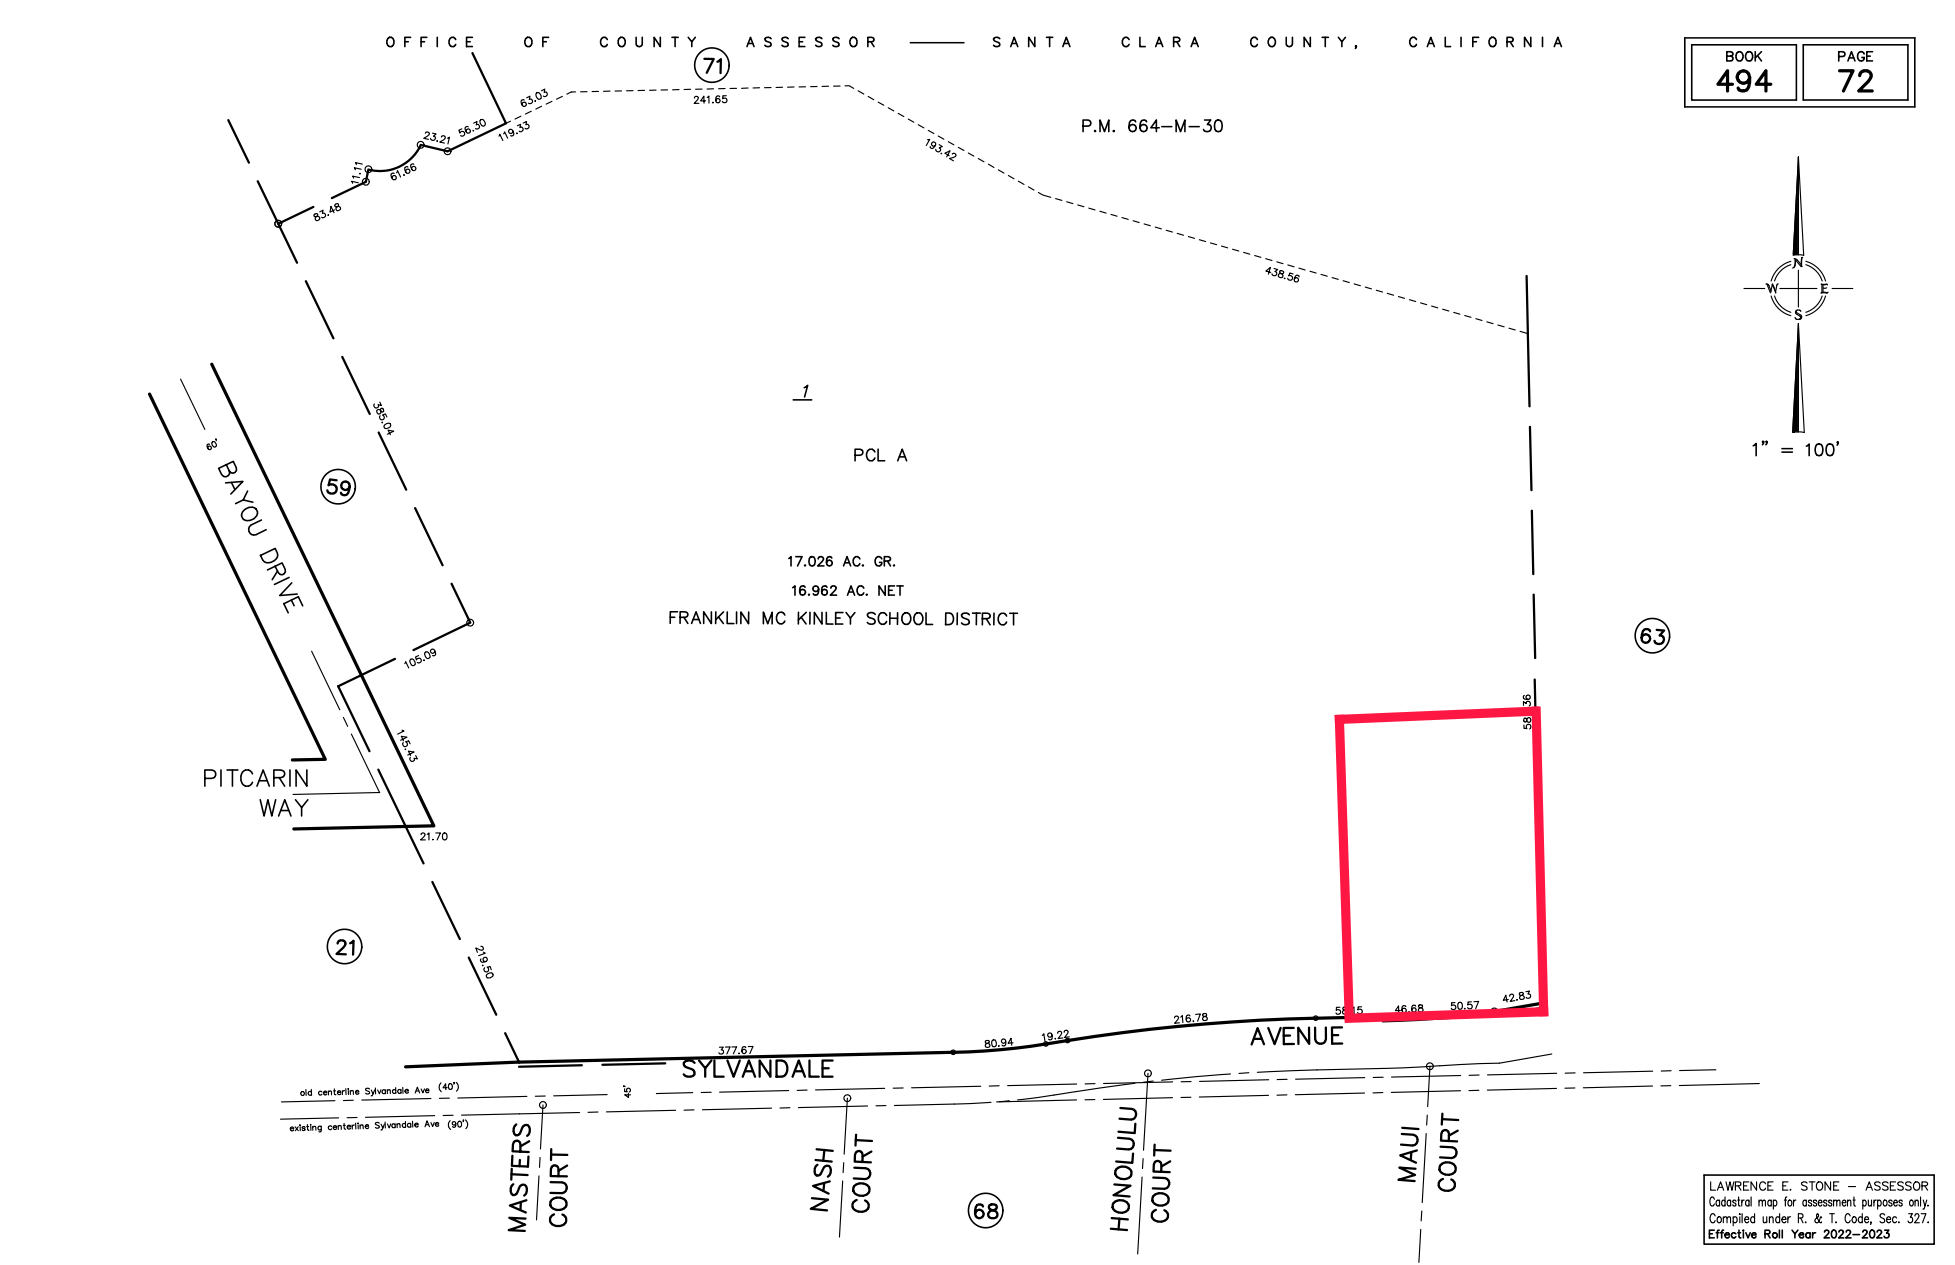
\includegraphics[width=\textwidth]{Assessor-Info/spark-academy-plat-map-494-72}\\ %chktex 8
    \footnotesize{Santa Clara County Assessor's Office (n.d.). [Plat Map]. Retrieved 07 Jan 2023 from  \url{https://tinyurl.com/spark-academy-plat-map}}.
    
    \noindent\footnotesize{Note: The outline is approximate.}
  \end{figure}

\begin{table}[hbt]
  \SingleSpacing%
  \caption[Spark Academy: Taxable Amount of Assessed Propery]{\textit{Spark Academy: Taxable Amount of Assessed Property}}\label{tab:spark-academy-taxable-amount}
  \begin{tabular}{llll}
    \toprule
    Year & Land        & Improvements & Total Assessed Value \\
    \midrule
    2022 & \$0         & \$0          & \\
    2021 & \$0         & \$0          & \\
    2020 & \$0         & \$0          & \\
    \bottomrule
  \end{tabular}\\
  \noindent\footnotesize{Note: As noted above, Spark Academy leases its land from the Franklin McKinley School District. Since public school districts are exempt from property taxes, all the taxable amounts in this table are listed as \$0.}
\end{table}

\begin{figure}[hbt]
  \centering
  \caption[Spark Academy Satellite Photo] {\textit{Spark Academy Satellite Photo}}\label{fig:spark-academy-sat-photo}
  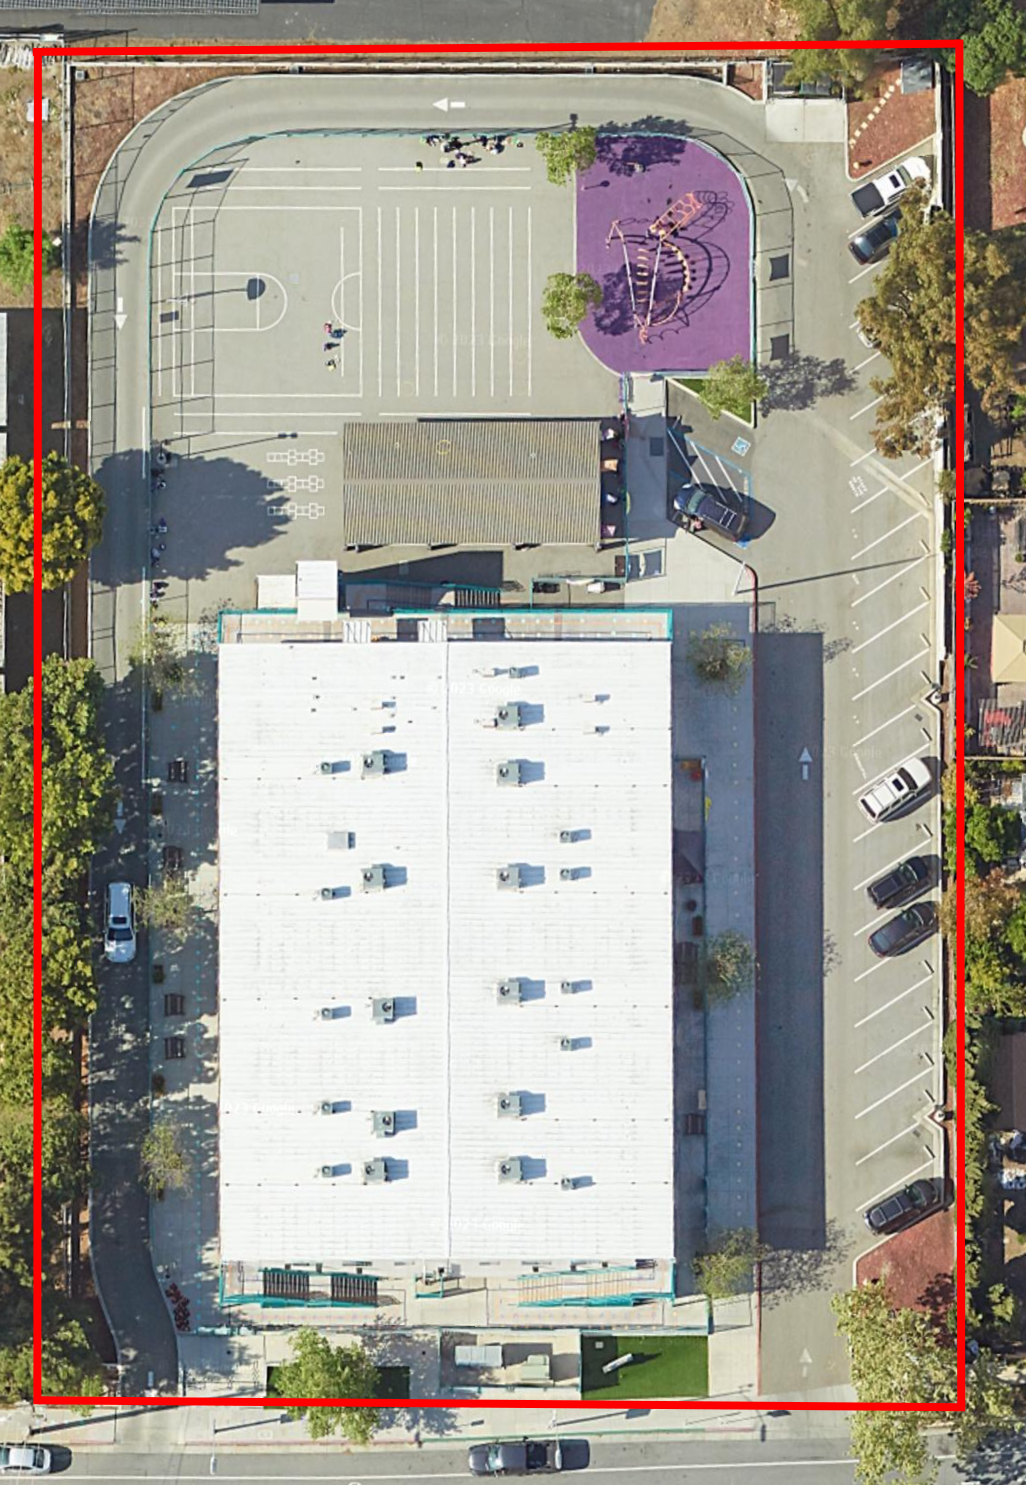
\includegraphics[height=0.6\textheight]{Satellite-Photos/spark-academy-sat-photo}\\ %chktex 8
  \footnotesize{Google. (n.d). [Google Earth image]. Retrieved 07 Jan 2023 from \url{https://tinyurl.com/spark-academy}.}
  \noindent\footnotesize{Note: The outline is approximate.}
\end{figure}

%%%%%%%%%%%%%%%%%%%%%%%%%%%%%%%%%%%%%%%%%%%%%%%%%%%%%%%%%%%%%%%%%%%%%%%%%%%%%%%%%%%%%%%%%%%%%%%%%%%%%%%%%%%%%%%%%%%%%%%%%

\clearpage
\section{Fuerza }\label{sec:fuerza-info}

\begin{table}[htb]
  \SingleSpacing%
  \caption[Fuerza: Property Information]{\textit{Fuerza: Property Information}}\label{tab:fuerza-prop-info}
  \begin{tabular}{ll}
    \toprule
    Property Address      & 70 S. Jackson Ave, San José, CA 95116 \\
    Assessor's Parcel No. & 484–41–162 \\
    Size                  & 1.35ac \\
    Date of Last Sale     & 02 Feb 2018 \\
    \bottomrule
  \end{tabular}
\end{table}

\begin{figure}[hbt]
    \caption[Fuerza Plat Map]{\textit{Fuerza Plat Map}}\label{fig:fuerza-plat-map}
    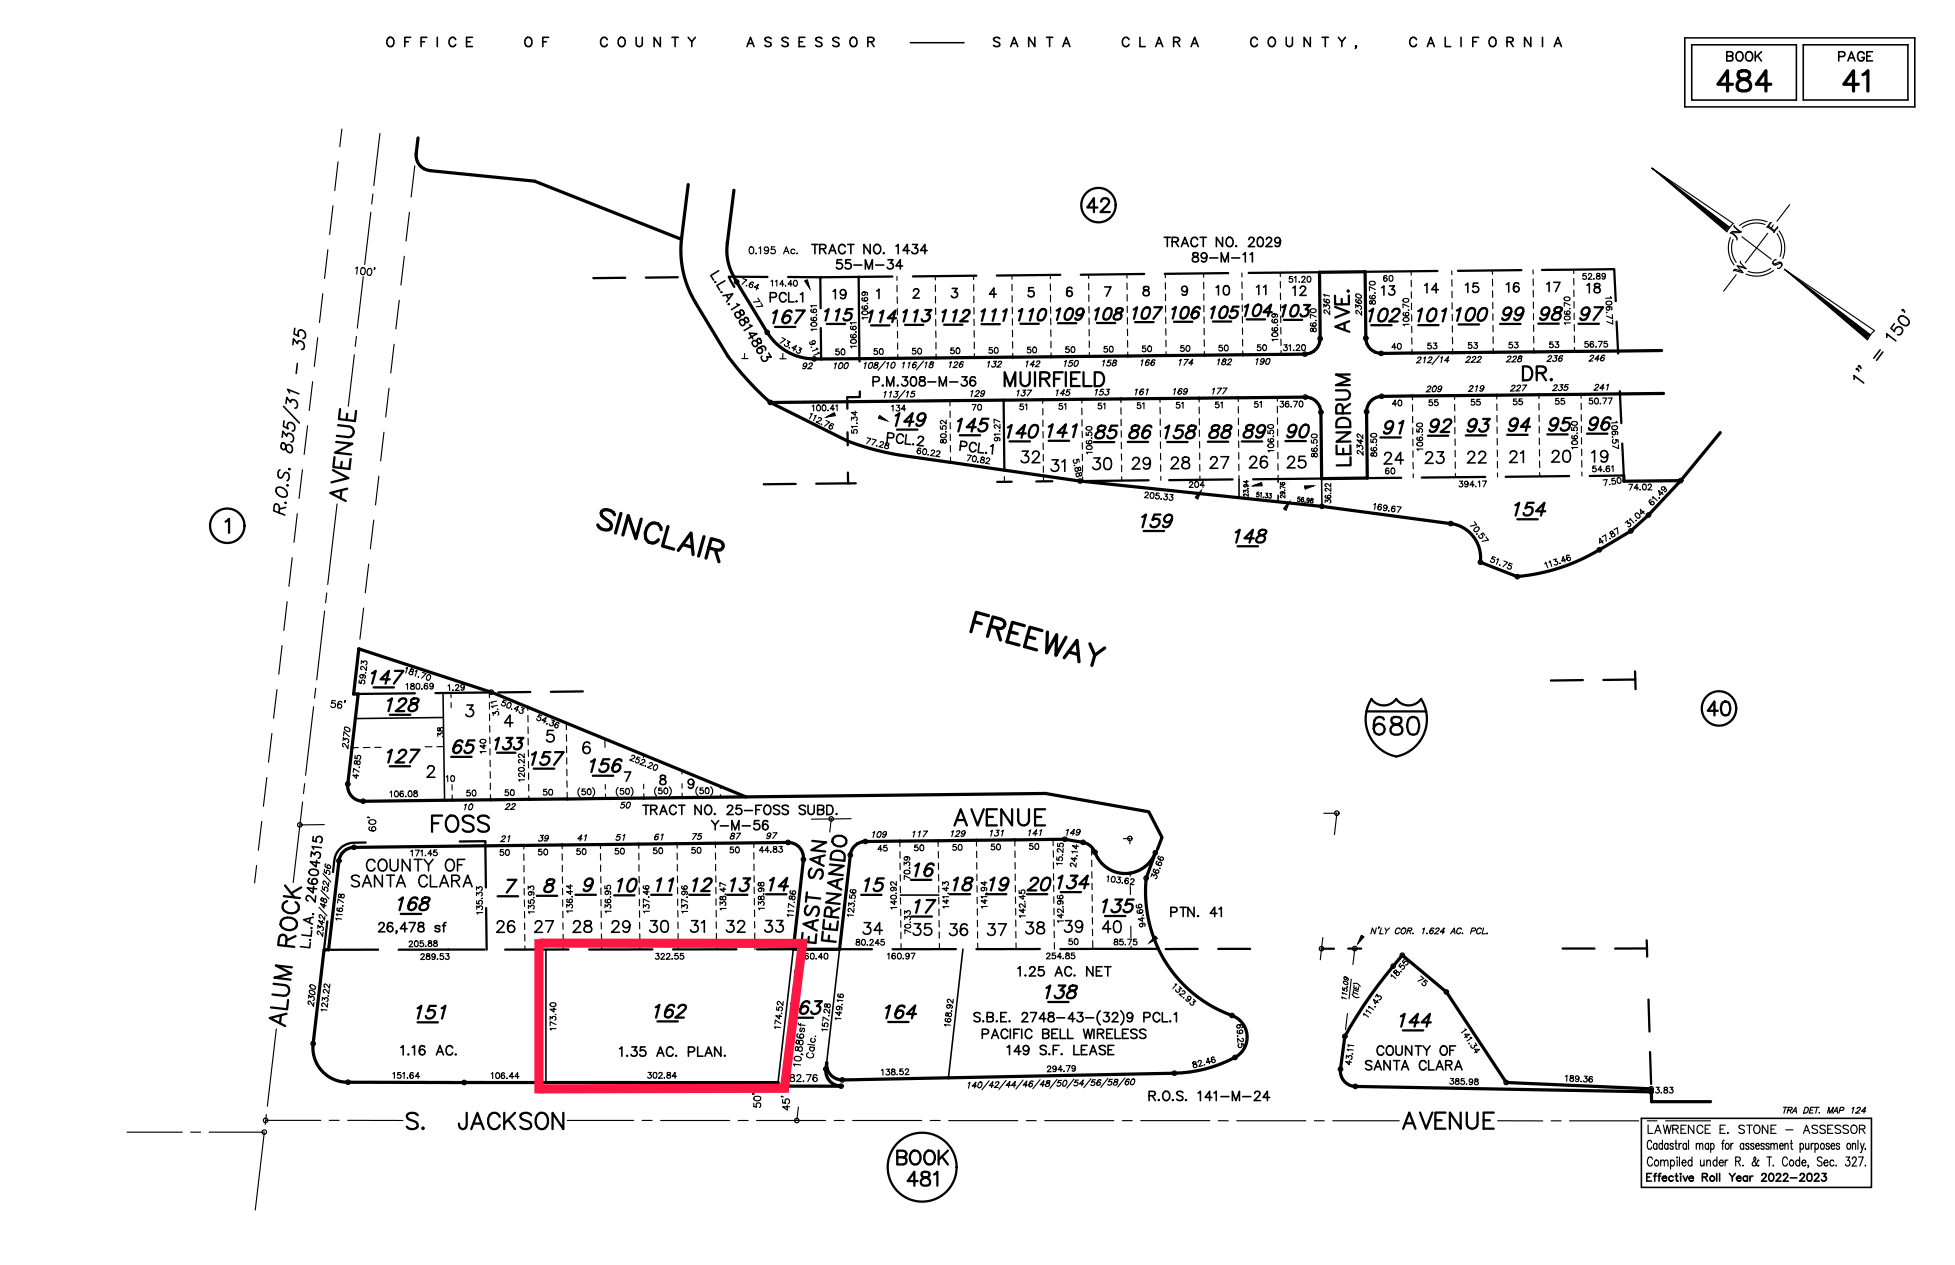
\includegraphics[width=\textwidth]{Assessor-Info/fuerza-plat-map-484-41}\\ %chktex 8
    \footnotesize{Santa Clara County Assessor's Office (n.d.). [Plat Map]. Retrieved 07 Jan 2023 from  \url{https://tinyurl.com/fuerza-plat-map}}.
\end{figure}

\begin{table}[hbt]
  \SingleSpacing%
  \caption[Fuerza: Taxable Amount of Assessed Propery]{\textit{Fuerza: Taxable Amount of Assessed Property}}\label{tab:fuerza-taxable-amount}
  \begin{tabular}{llll}
    \toprule
    Year & Land        & Improvements & Total Assessed Value \\
    \midrule
    2022 & \$2,656,862 & \$937,117    & \$3,593,979 \\
    2021 & \$2,604,767 & \$918,743    & \$3,523,510 \\
    2020 & \$2,578,059 & \$909,323    & \$3,487,382 \\
    \bottomrule
  \end{tabular}
\end{table}

\begin{figure}[hbt]
  \caption[Fuerza Satellite Photo]{\textit{Fuerza Satellite Photo}}\label{fig:fuerza-sat-photo}
  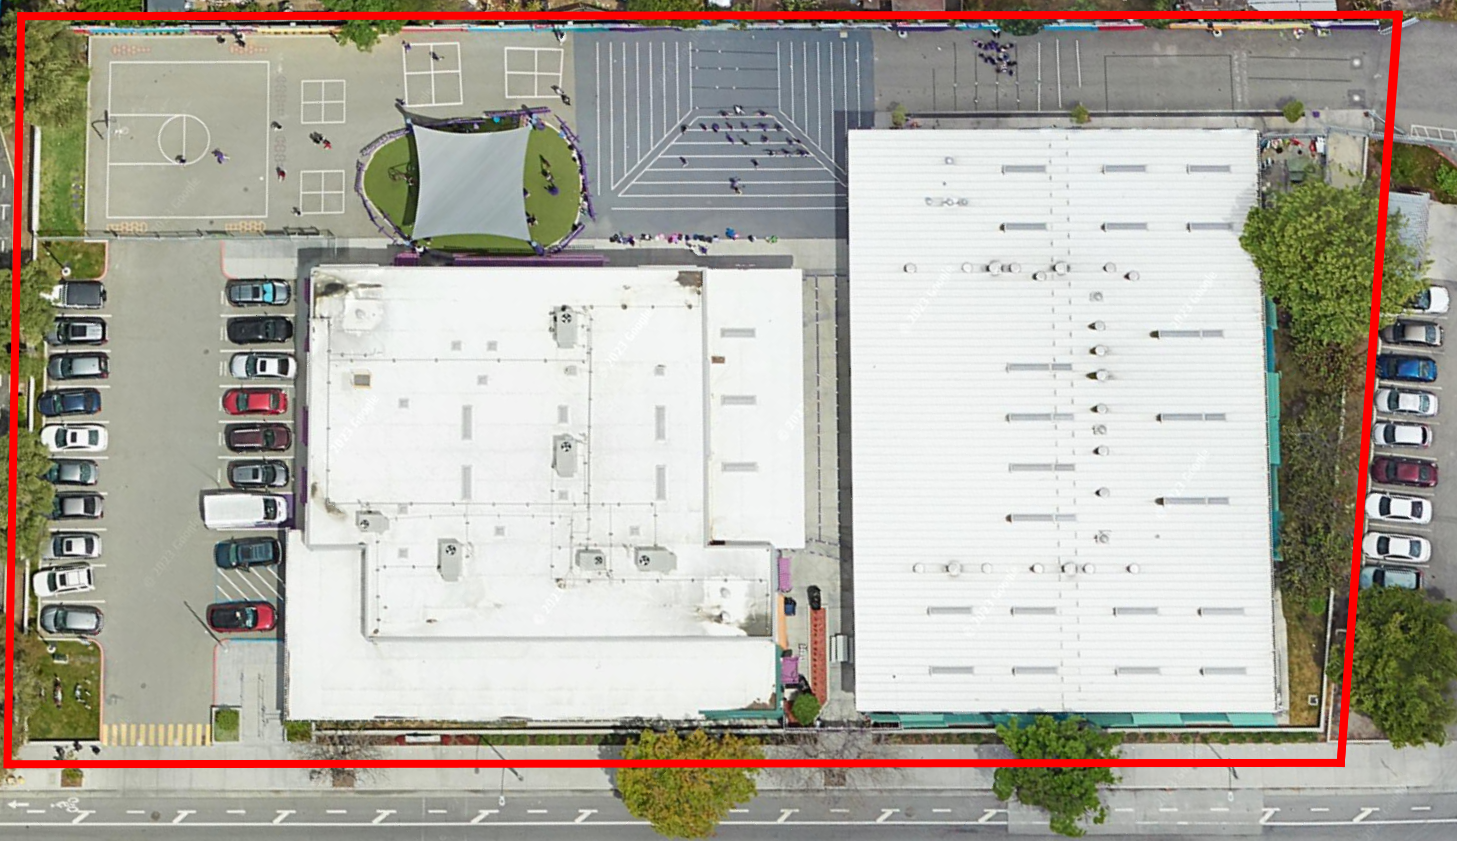
\includegraphics[width=\textwidth]{Satellite-Photos/fuerza-sat-photo}\\ %chktex 8
  \footnotesize{Google. (n.d). [Google Earth image]. Retrieved 07 Jan 2023 from \url{https://tinyurl.com/fuerza-v2}.}
\end{figure}

%%%%%%%%%%%%%%%%%%%%%%%%%%%%%%%%%%%%%%%%%%%%%%%%%%%%%%%%%%%%%%%%%%%%%%%%%%%%%%%%%%%%%%%%%%%%%%%%%%%%%%%%%%%%%%%%%%%%%%%%%

\clearpage
\section{Rising Stars}\label{sec:rising-stars-info}

\begin{table}[htb]
  \SingleSpacing%
  \caption[Rising Stars: Property Information]{\textit{Rising Stars: Property Information}}\label{tab:rising-stars-prop-info}
  \begin{tabular}{ll}
    \toprule
    Property Address      & 3173 Senter Road, San José, CA 95111 \\
    Assessor's Parcel No. & 494–01–027 \\
    Size                  & 1.58ac \\
    Date of Last Sale     & 01 Dec 2016 \\
    \bottomrule
  \end{tabular}
\end{table}

\begin{figure}[hbt]
    \caption[Rising Stars Plat Map]{\textit{Rising Stars Plat Map}}\label{fig:rising-stars-plat-map}
    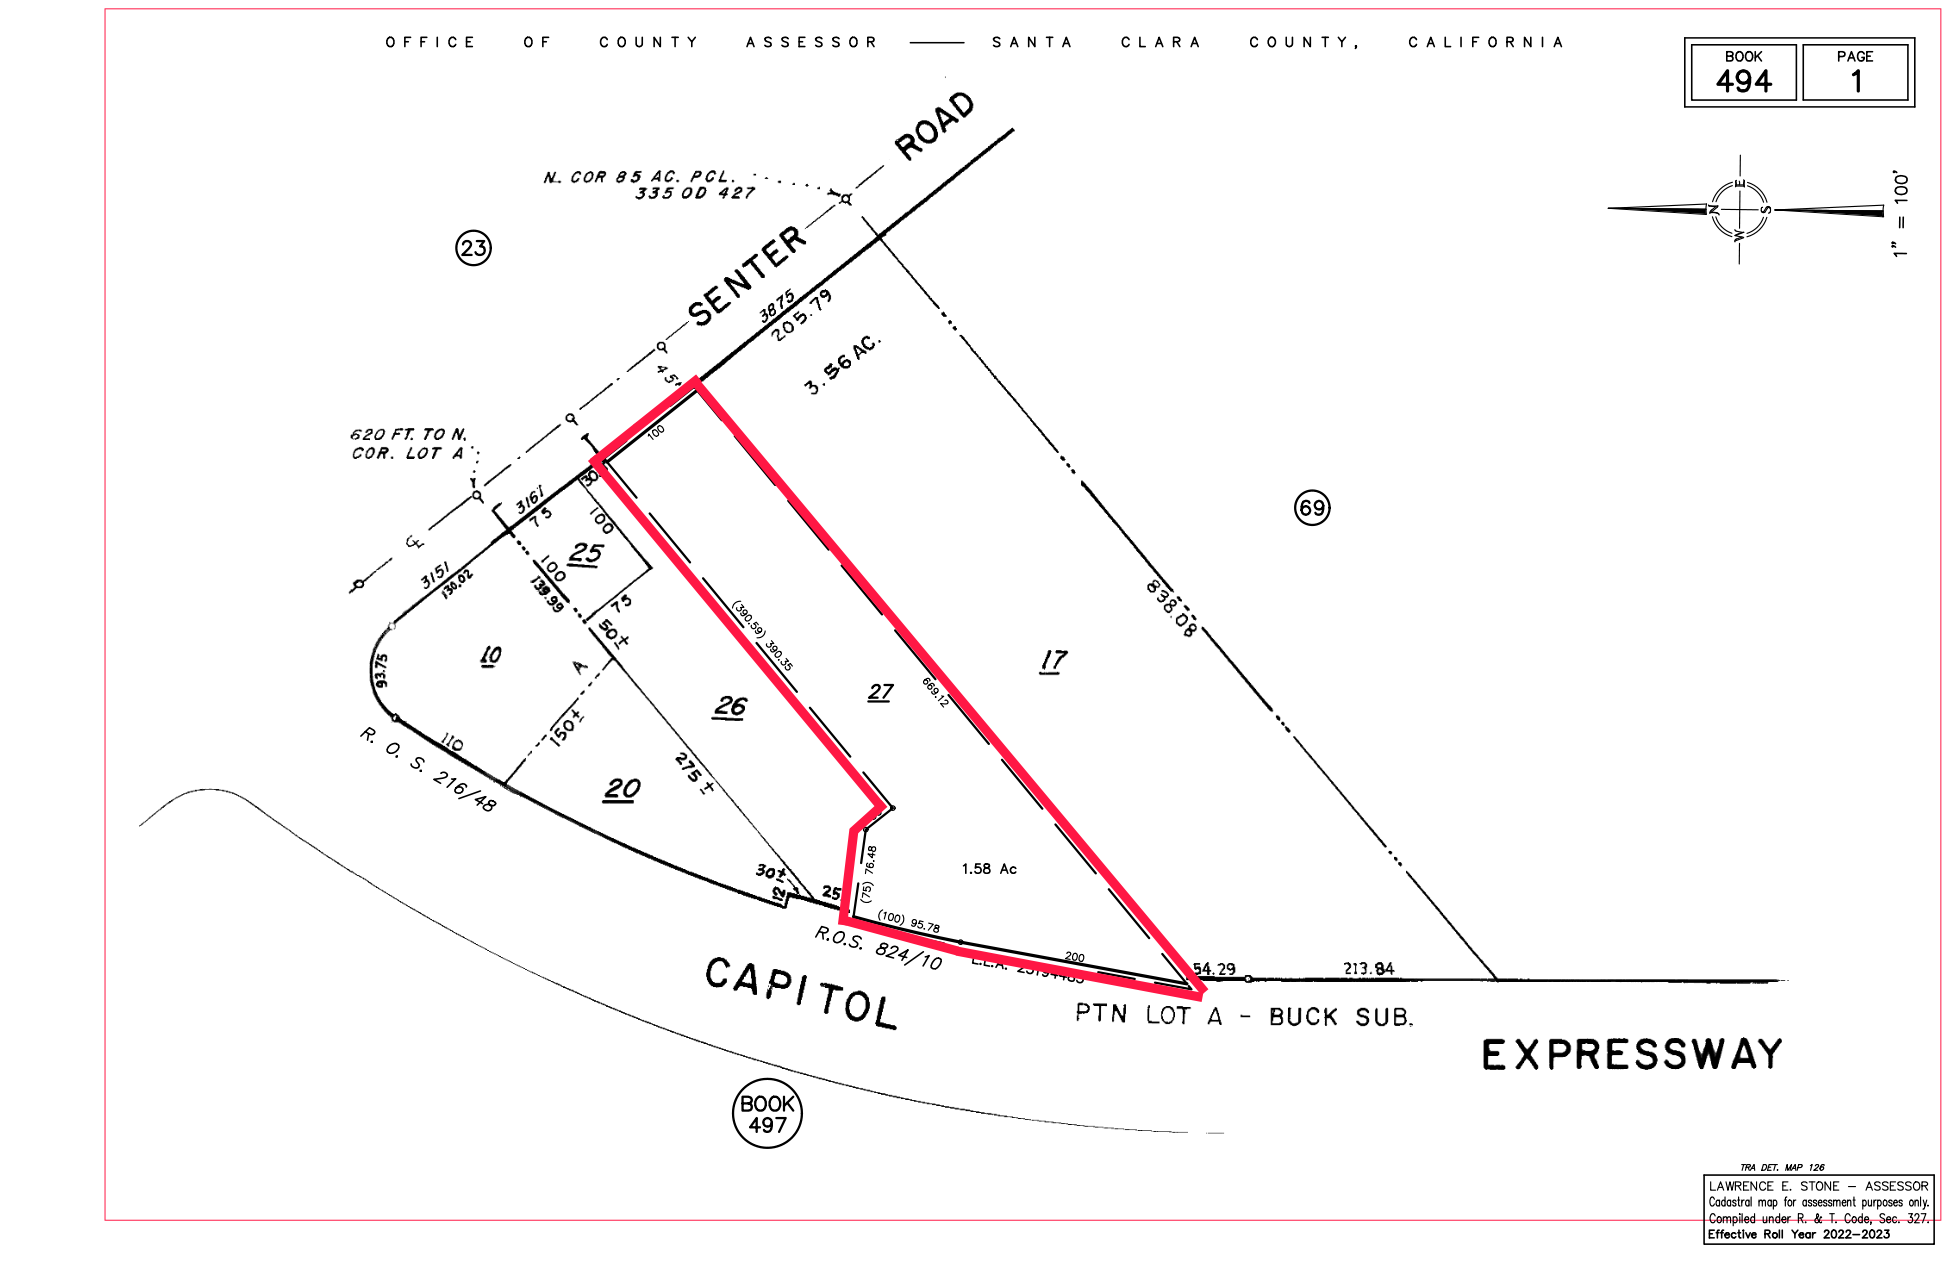
\includegraphics[width=\textwidth]{Assessor-Info/rising-stars-plat-map-494-01}\\ %chktex 8
    \footnotesize{Santa Clara County Assessor's Office (n.d.). [Plat Map]. Retrieved 07 Jan 2023 from  \url{https://tinyurl.com/rising-stars-plat-map}}.
\end{figure}

\begin{table}[hbt]
  \SingleSpacing%
  \caption[Rising Stars: Taxable Amount of Assessed Propery]{\textit{Rising Stars: Taxable Amount of Assessed Property}}\label{tab:rising-stars-taxable-amount}
  \begin{tabular}{llll}
    \toprule
    Year & Land        & Improvements & Total Assessed Value \\
    \midrule
    2022 & \$2,997,872 & \$12,139,470 & \$15,137,342 \\
    2021 & \$2,939,091 & \$11,901,442 & \$12,139,470 \\
    2020 & \$2,908,955 & \$11,779,408 & \$14,688,363 \\
    \bottomrule
  \end{tabular}
\end{table}

\begin{figure}[hbt]
  \centering
  \caption[Rising Stars Satellite Photo]{\textit{Rising Stars Satellite Photo}}\label{fig:rising-stars-sat-photo}
  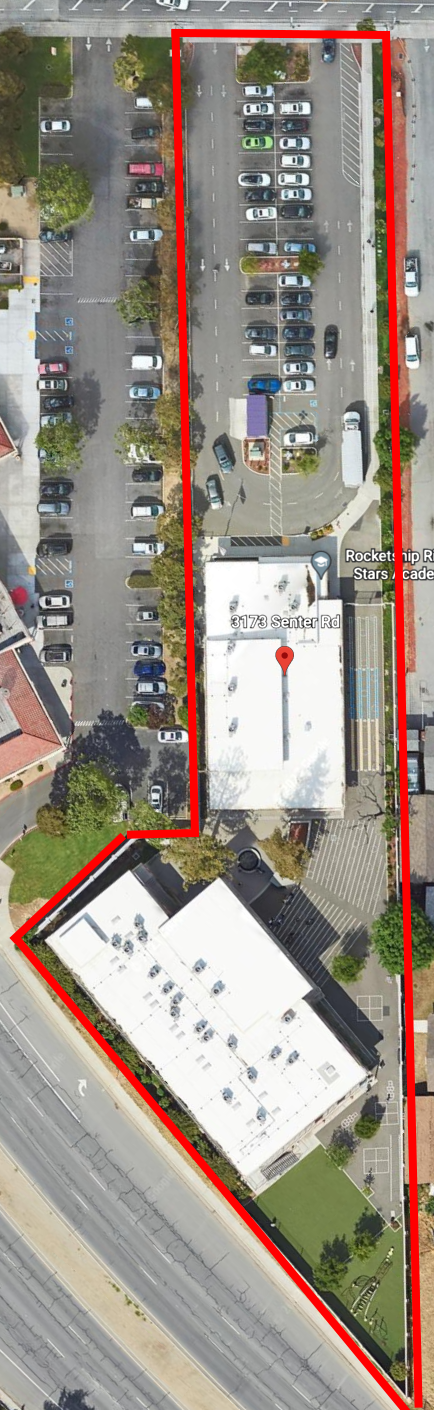
\includegraphics[height=0.667\textheight]{Satellite-Photos/rising-stars-sat-photo}\\ %chktex 8
  \footnotesize{Google. (n.d). [Google Earth image]. Retrieved 07 Jan 2023 from \url{https://tinyurl.com/rising-stars-v2}.}
\end{figure}

%%% Local Variables:
%%% mode: latex
%%% TeX-master: "Rocketship_Education-An_Exploratory_Public_Policy_Case_Study"
%%% End:

\clearforchapter%%% Time-stamp: <2023-05-07 17:03:09 vladimir>
%%% Copyright (C) 2019-2023 Vladimir G. Ivanović
%%% Author: Vladimir G. Ivanović <vladimir@acm.org>
%%% ORCID: https://orcid.org/0000-0002-7802-7970

\chapter{Consolidated Financial Position}\label{ch:consolidated_financial_position}
\begin{figure}[hbt]
    \caption[Consolidated Financial Position, Years Ending 2010–2022]{\textit{Consolidated Financial Position, Years Ending 2010-2022}}\label{fig:consolidated_financial_position_2010-2022-1} %chktex 8
    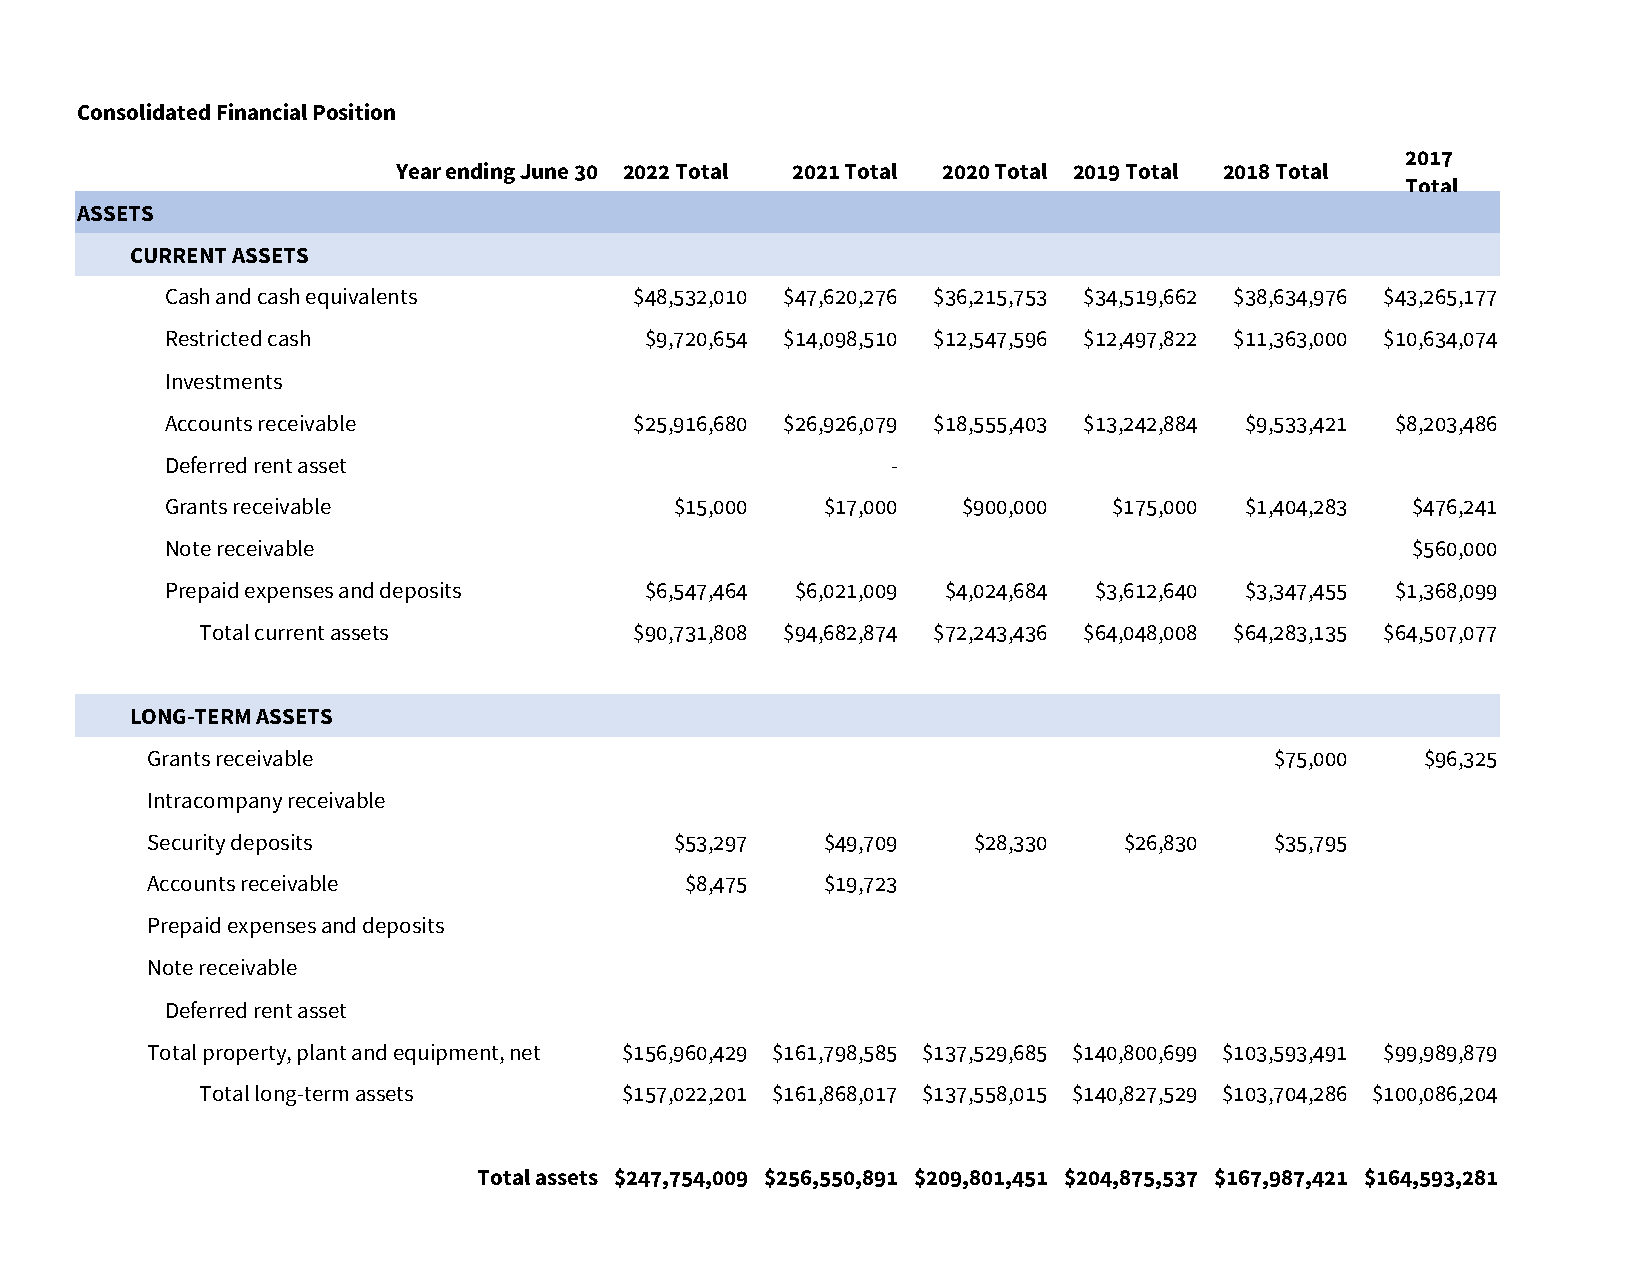
\includegraphics[width=\textwidth]{Consolidated Financial Statements/v5 Spreadsheets/Consolidated_Financial_Position_Years_2010-2022 PDF pages/.pg_0001}\\ %chktex 8
\end{figure}
\begin{figure}[hbt]
    \caption[Consolidated Financial Position, Years Ending 2010–2022]{\textit{Consolidated Financial Position, Years Ending 2010-2022}}\label{fig:consolidated_financial_position_2010-2022-2} %chktex 8
    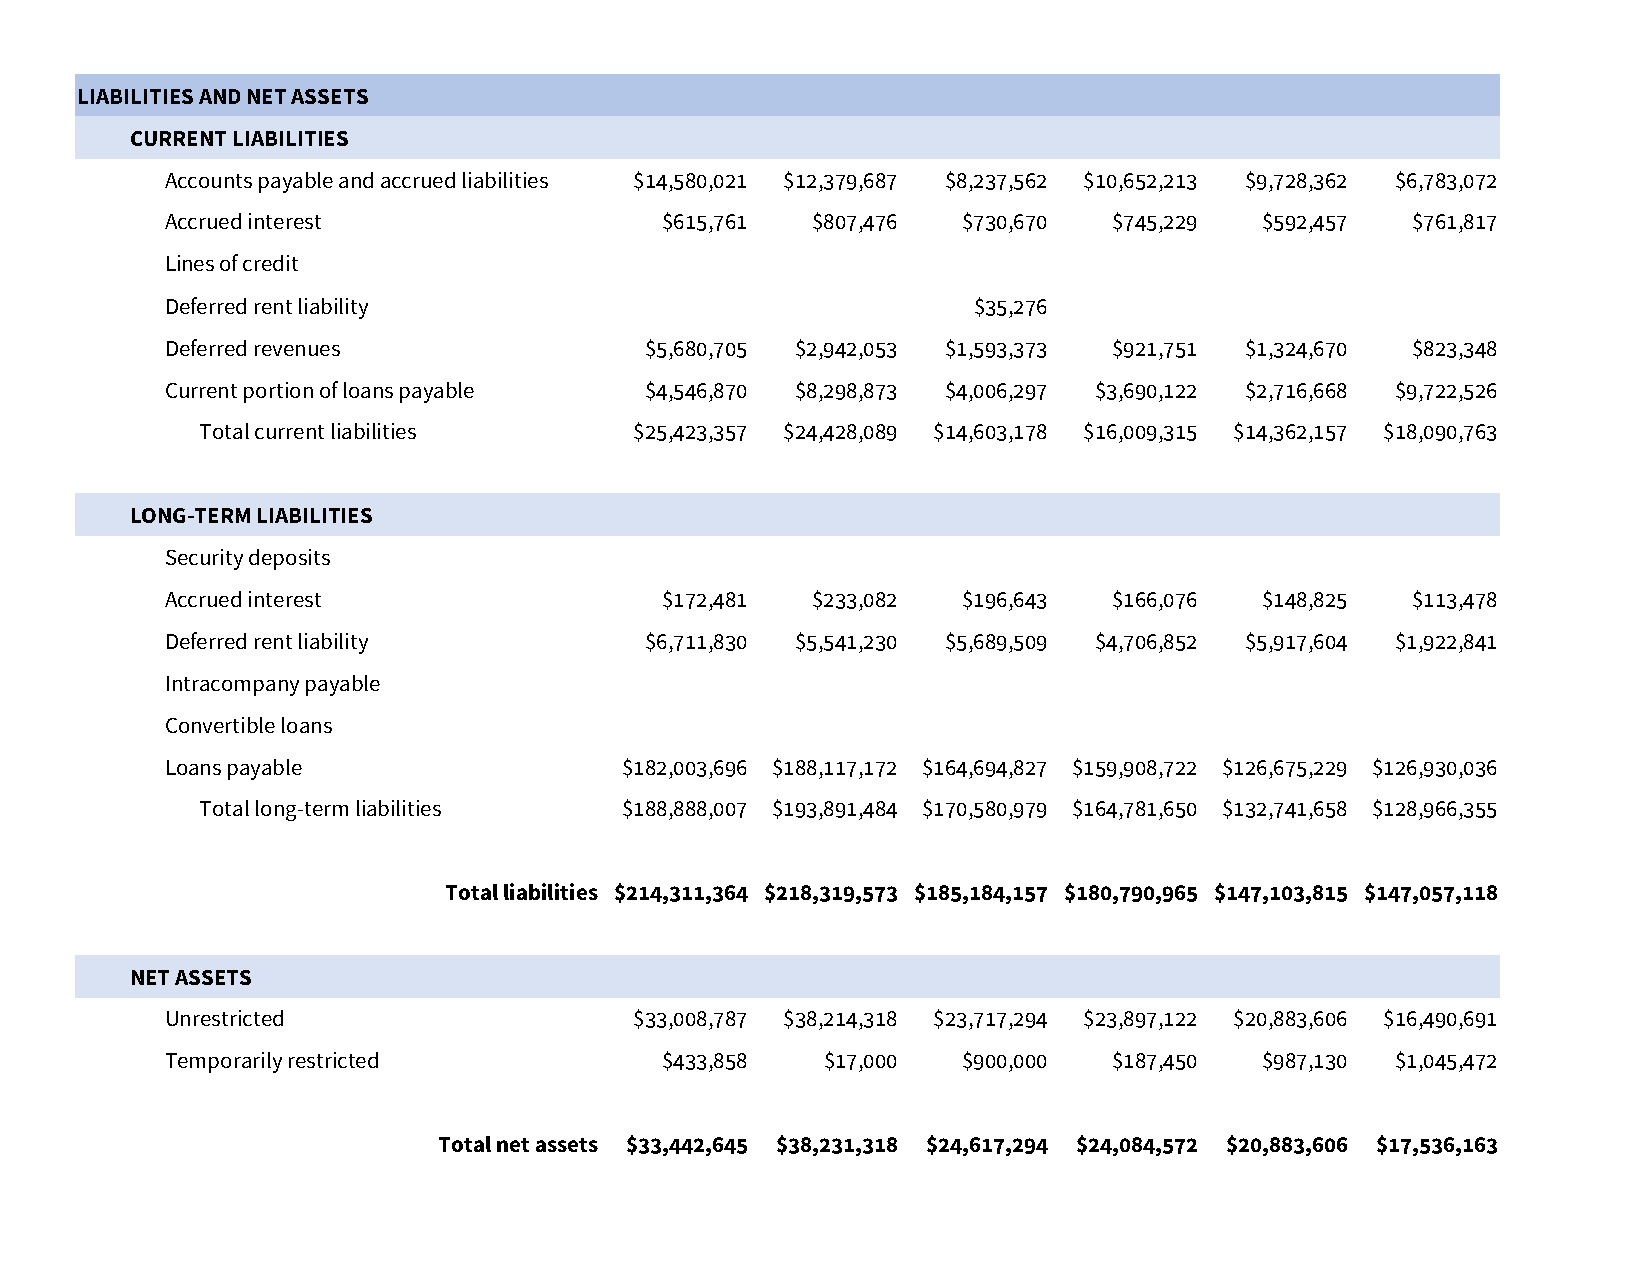
\includegraphics[width=\textwidth]{Consolidated Financial Statements/v5 Spreadsheets/Consolidated_Financial_Position_Years_2010-2022 PDF pages/.pg_0002}\\ %chktex 8
\end{figure}
\begin{figure}[hbt]
    \caption[Consolidated Financial Position, Years Ending 2010–2022]{\textit{Consolidated Financial Position, Years Ending 2010-2022}}\label{fig:consolidated_financial_position_2010-2022-3} %chktex 8
    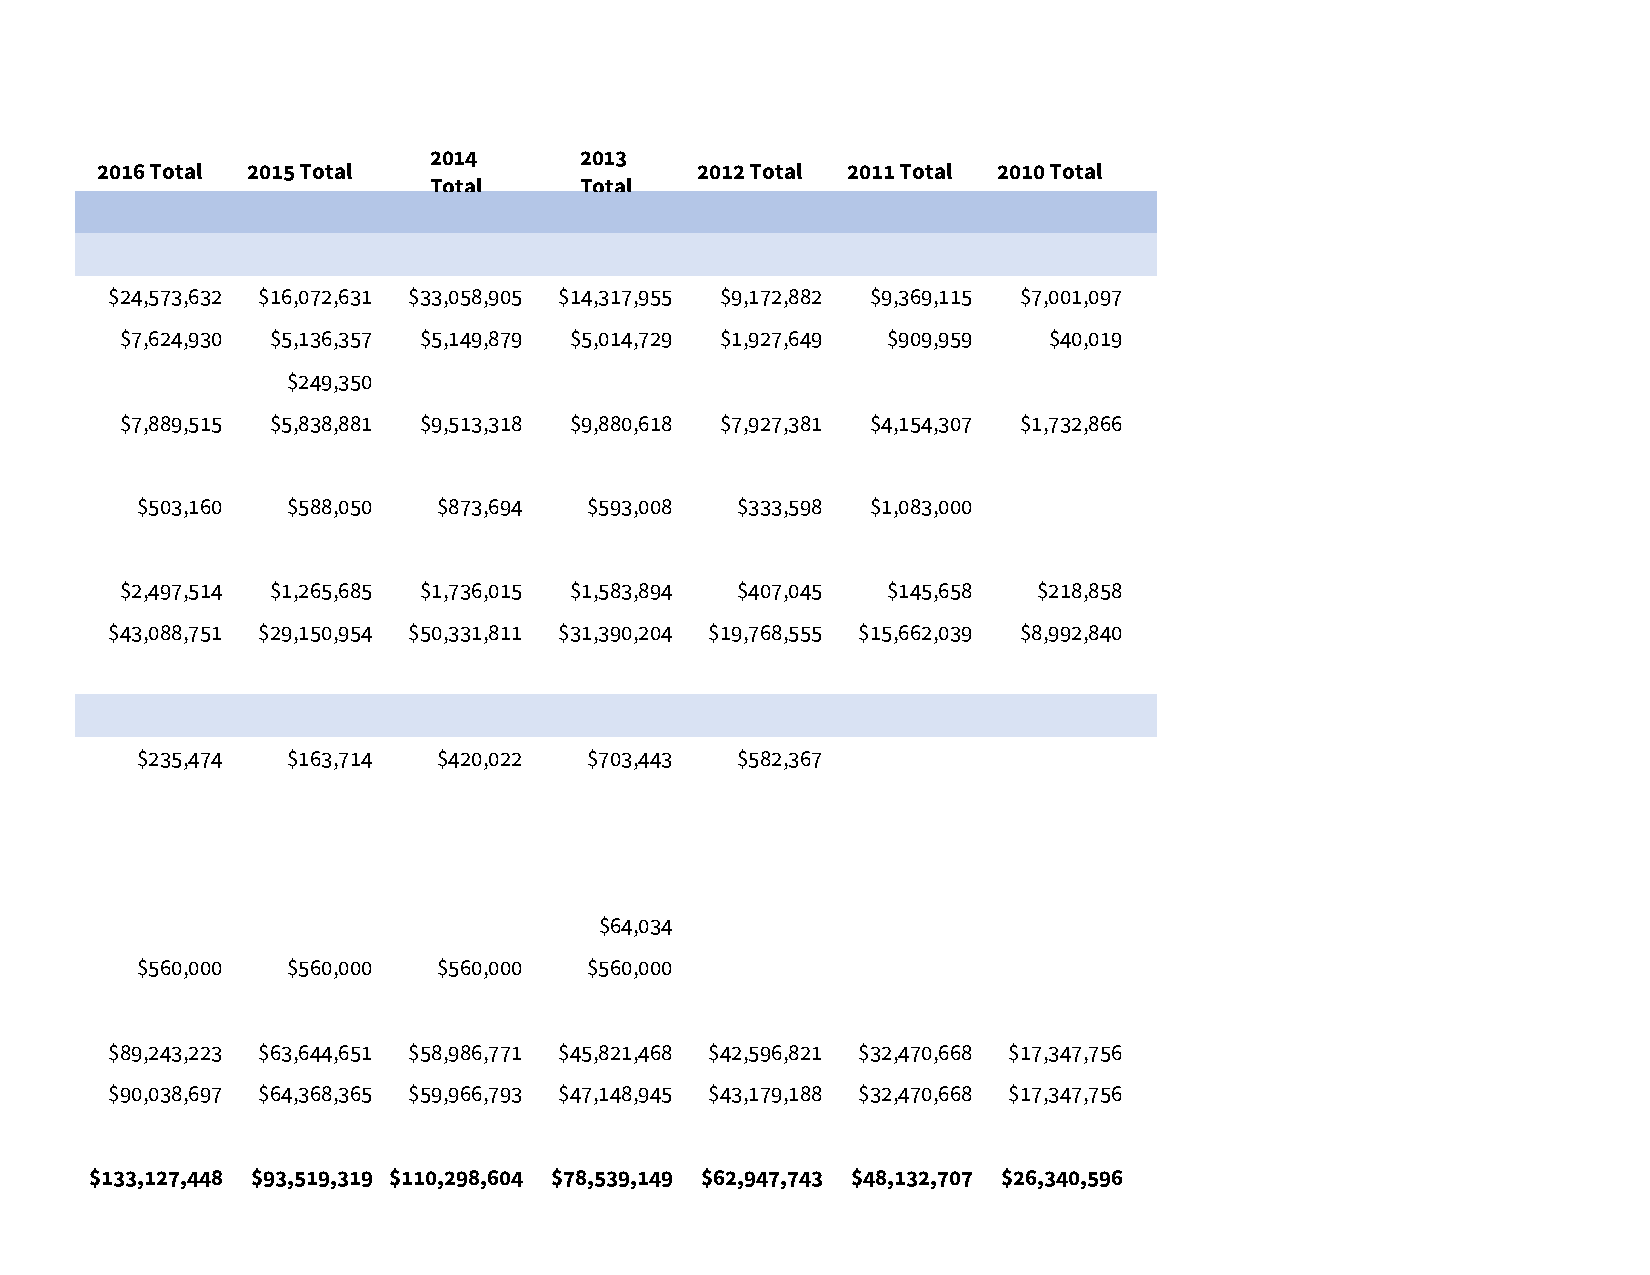
\includegraphics[width=\textwidth]{Consolidated Financial Statements/v5 Spreadsheets/Consolidated_Financial_Position_Years_2010-2022 PDF pages/.pg_0003}\\ %chktex 8
\end{figure}
\begin{figure}[hbt]
    \caption[Consolidated Financial Position, Years Ending 2010–2022]{\textit{Consolidated Financial Position, Years Ending 2010-2022}}\label{fig:consolidated_financial_position_2010-2022-4} %chktex 8
    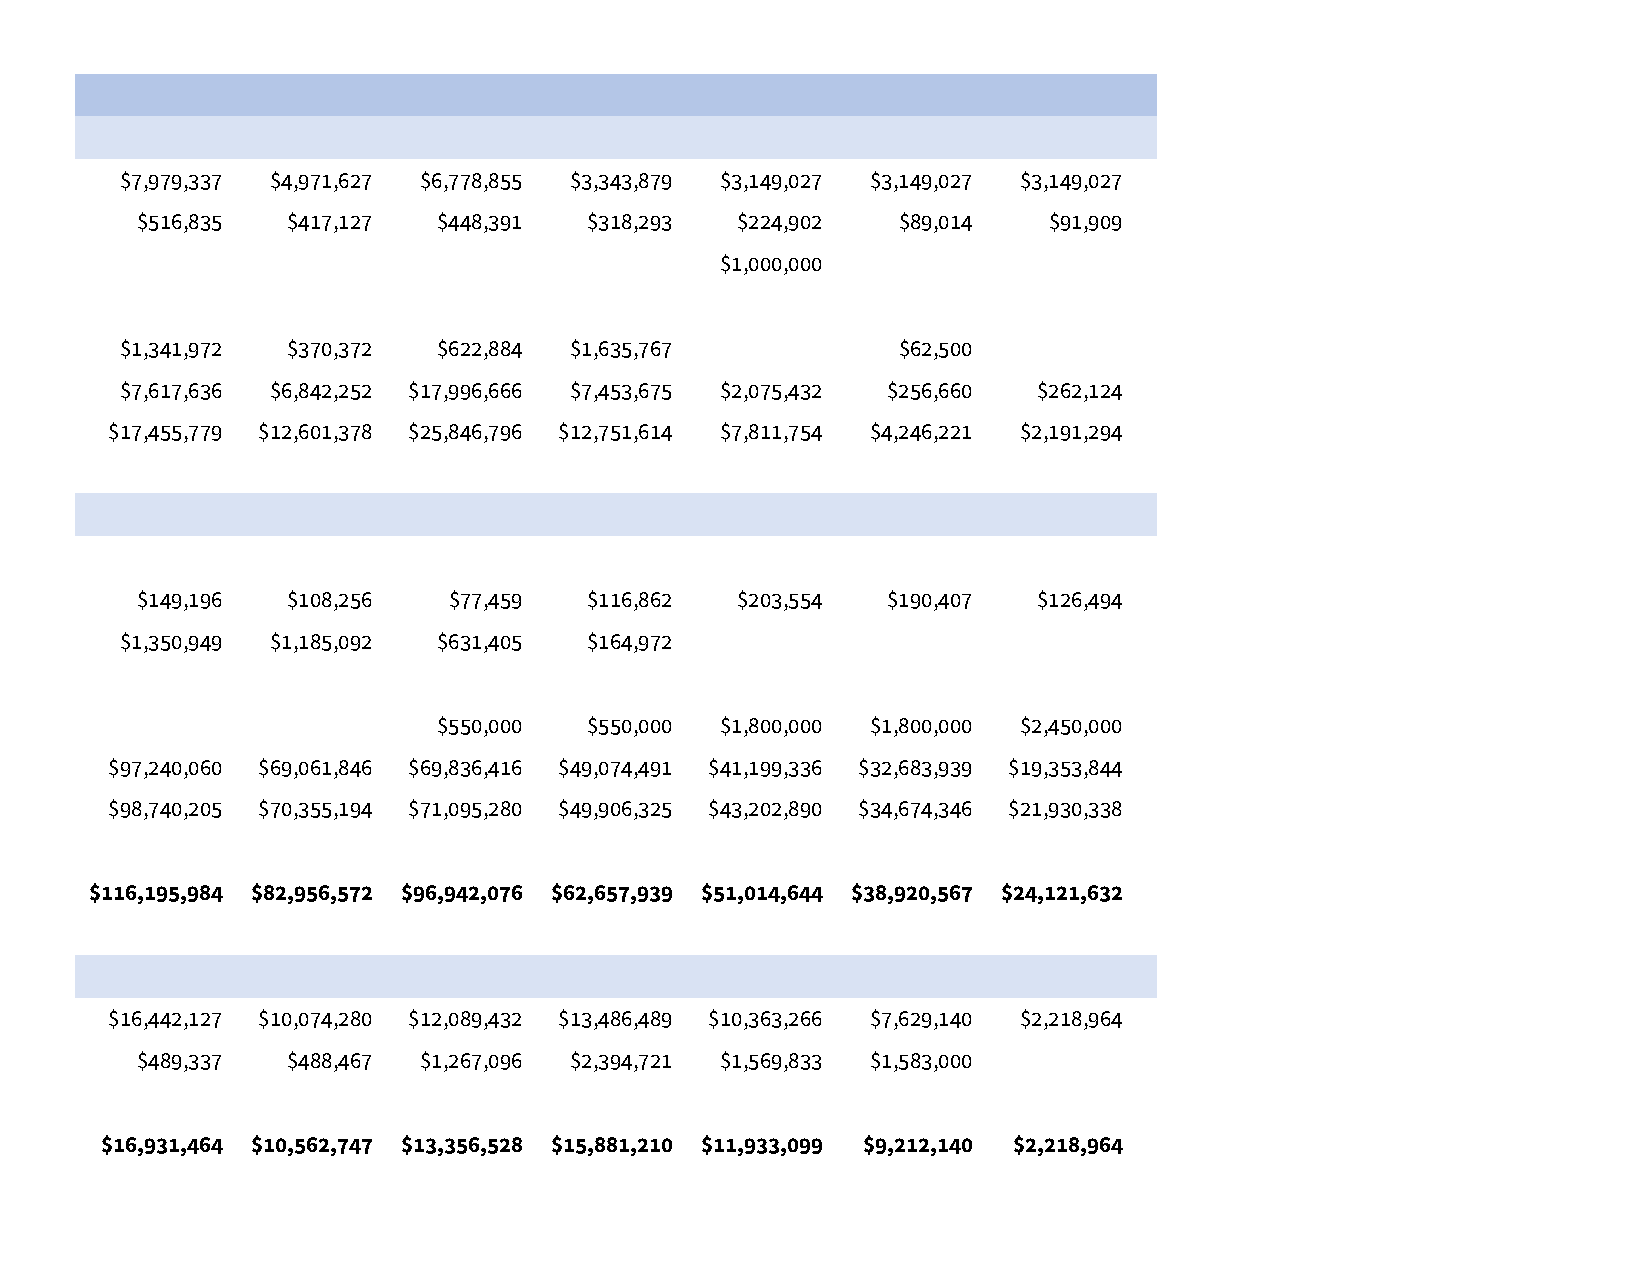
\includegraphics[width=\textwidth]{Consolidated Financial Statements/v5 Spreadsheets/Consolidated_Financial_Position_Years_2010-2022 PDF pages/.pg_0004}\\ %chktex 8
\end{figure}

%%% Local Variables:
%%% mode: latex
%%% TeX-master: "Rocketship_Education-An_Exploratory_Public_Policy_Case_Study"
%%% End:

\clearforchapter%%% Time-stamp: <2023-07-19 16:18:44 vladimir>
%%% Copyright (C) 2019-2023 Vladimir G. Ivanović
%%% Author: Vladimir G. Ivanović <vladimir@acm.org>
%%% ORCID: https://orcid.org/0000-0002-7802-7970

\chapter{Consolidated Activities (2010-2022)}\label{ch:consolidated_activities_2010-22}

  \begin{sidewaysfigure}
    \caption[Consolidated Activities, Years Ending 2010–2022]{\textit{Consolidated Activities, Years Ending 2010-2022}}\label{fig:consolidated_activities_2010-2022-4} %chktex 8
    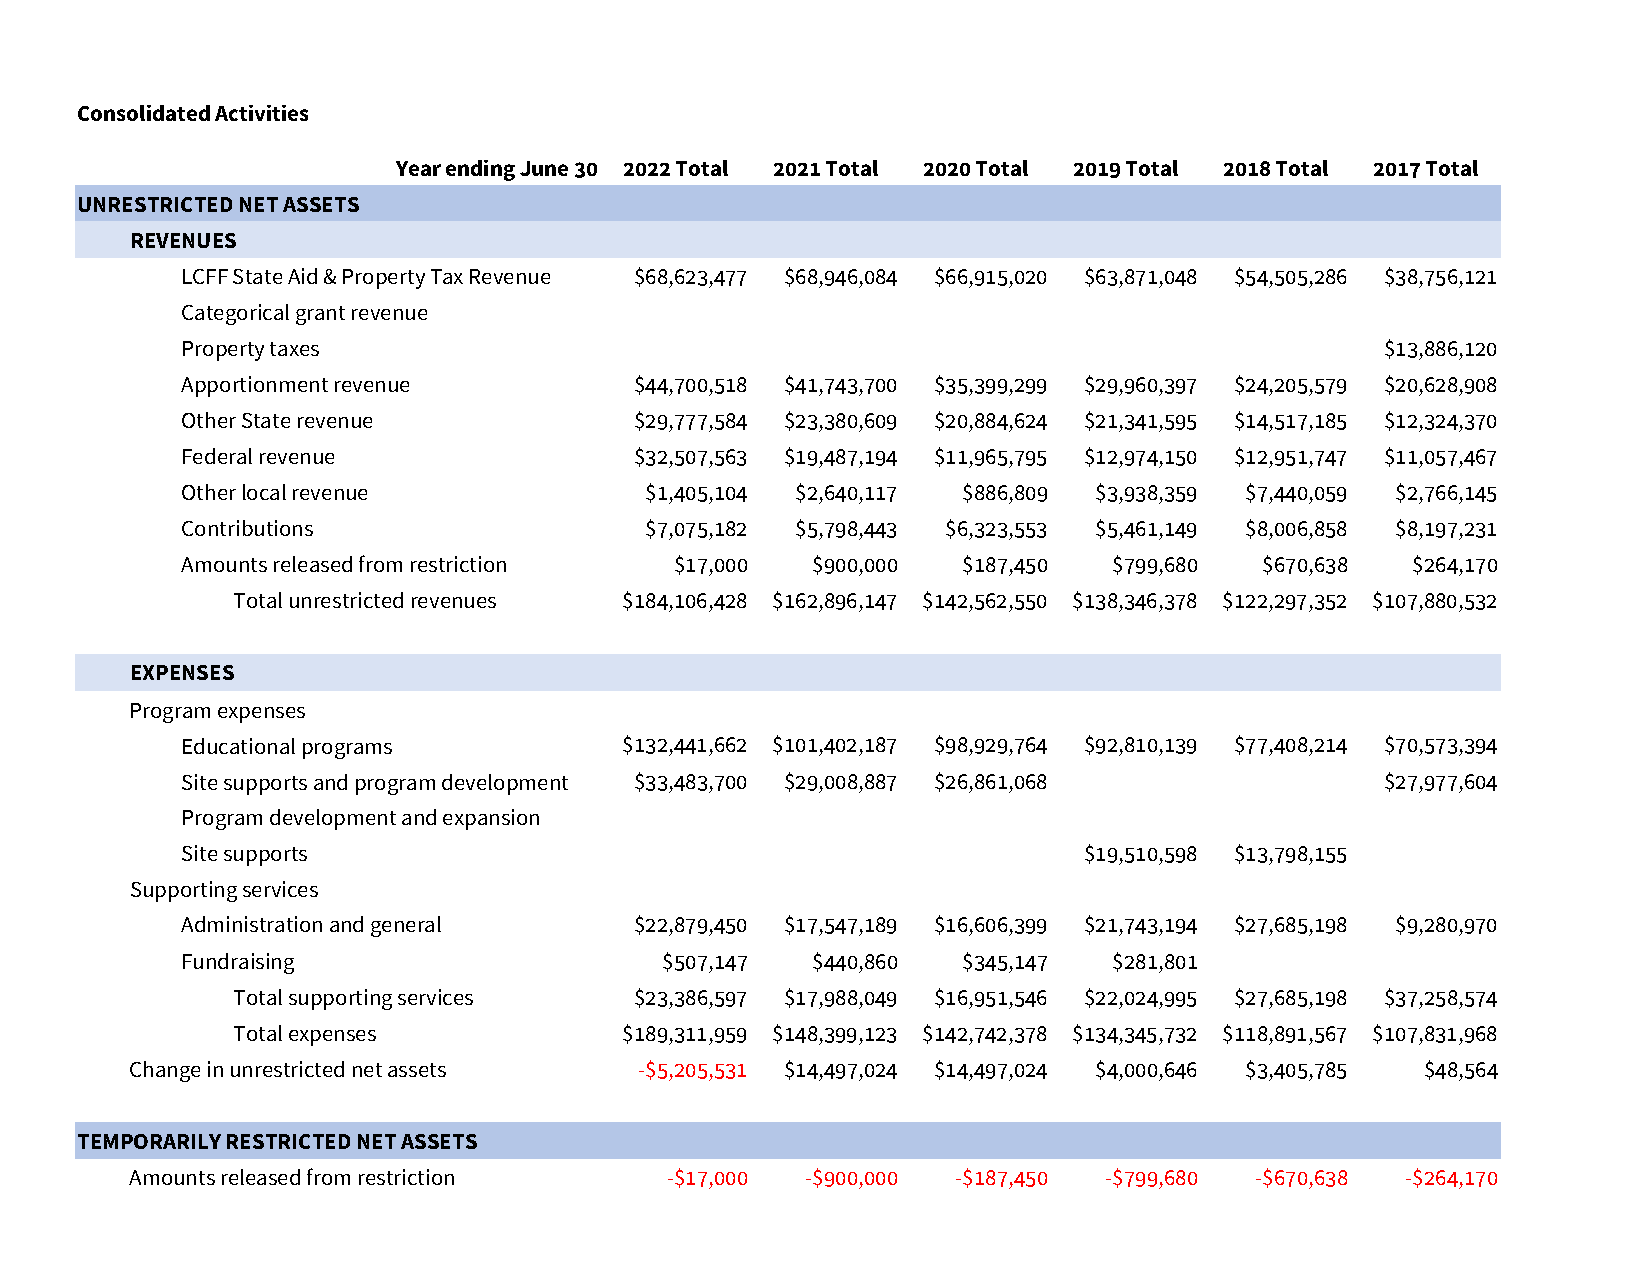
\includegraphics[width=0.9\textheight]{Consolidated_Financial_Statements/Consolidated_Activities_Years_2010-2022.pdf}\\ %chktex 8
  \end{sidewaysfigure}

% \begin{figure}[hbt]
%     \caption[Consolidated Financial Position, Years Ending 2010–2022]{\textit{Consolidated Activities, Years Ending 2010-2022}}\label{fig:consolidated_activities_2010-2022-1} %chktex 8
%     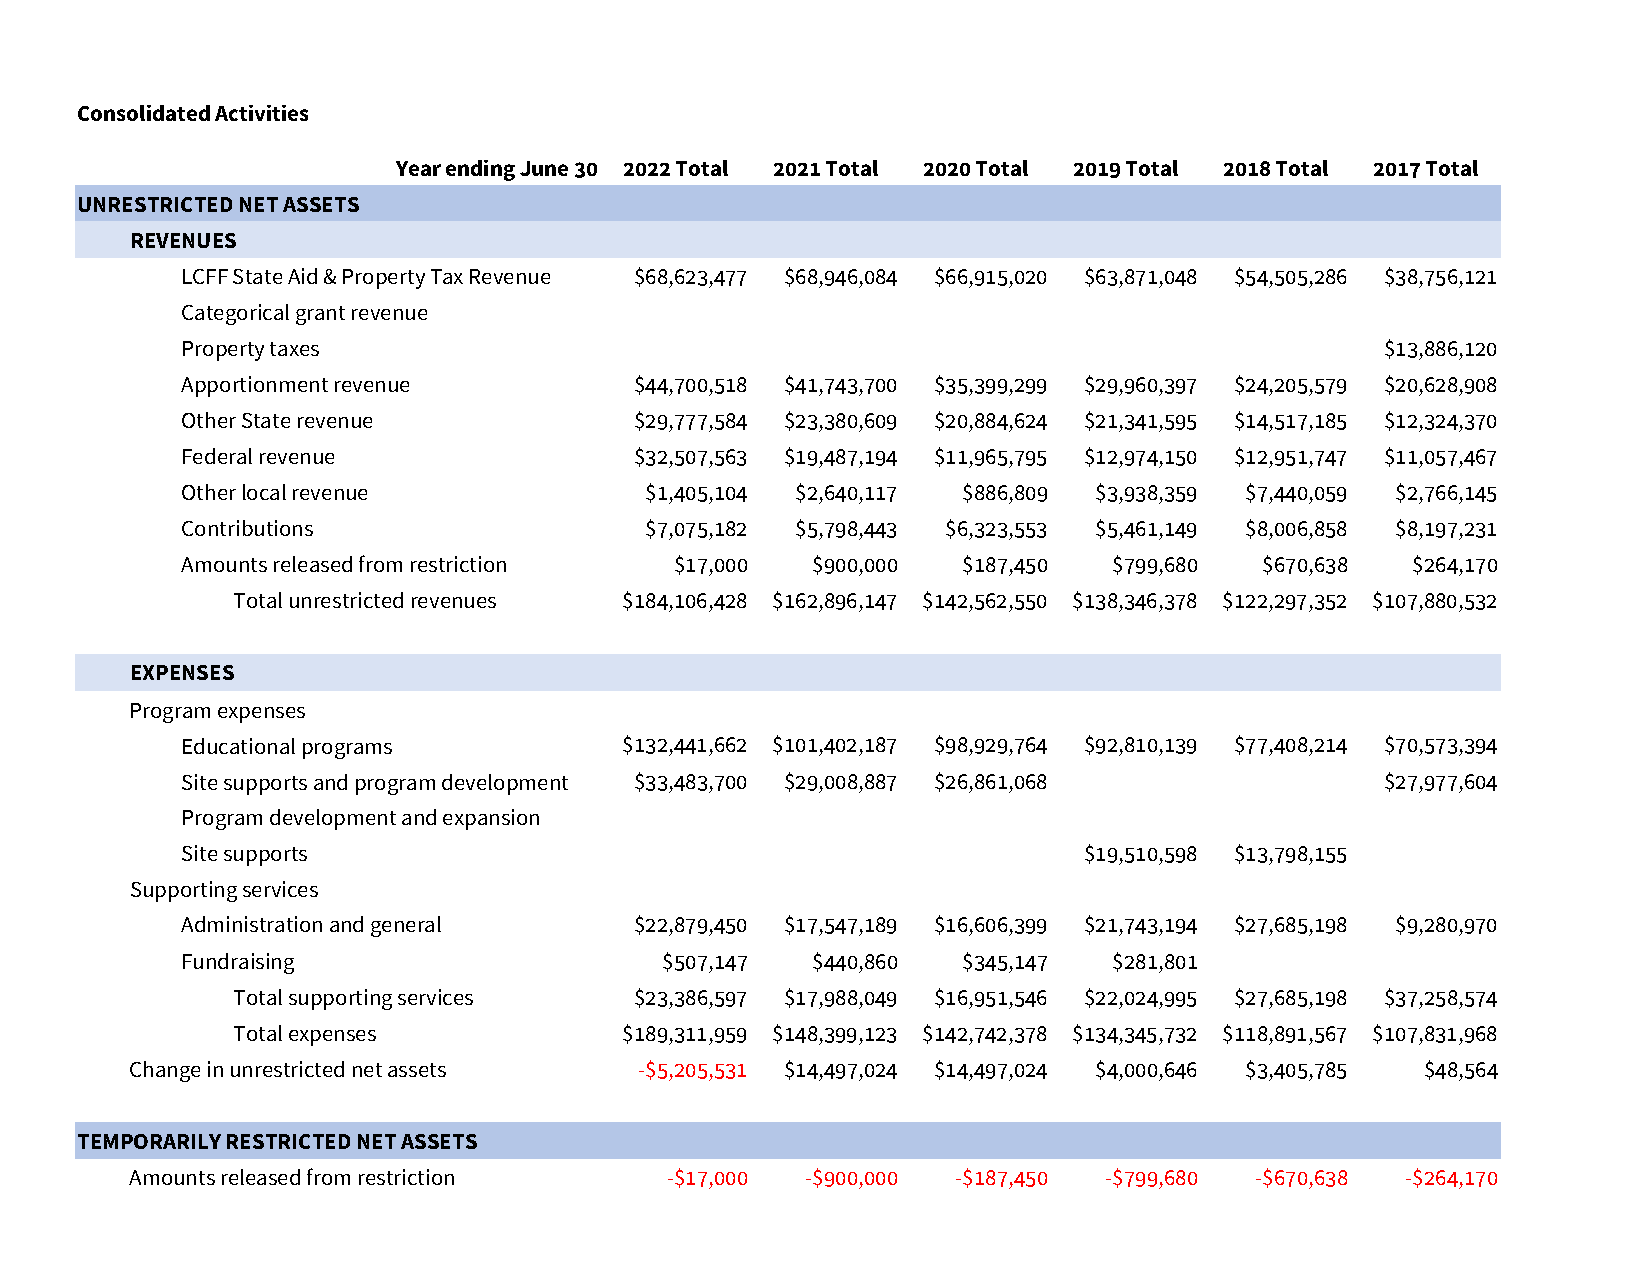
\includegraphics[width=\textwidth]{Consolidated Financial Statements/v5_Spreadsheets/Consolidated_Activities_Years_2010-2022 PDF pages/.pg_0001.pdf}\\ %chktex 8
% \end{figure}

% \begin{figure}[hbt]
%     \caption[Consolidated Activities, Years Ending 2010–2022]{\textit{Consolidated Activities, Years Ending 2010-2022}}\label{fig:consolidated_activities_2010-2022-2} %chktex 8
%     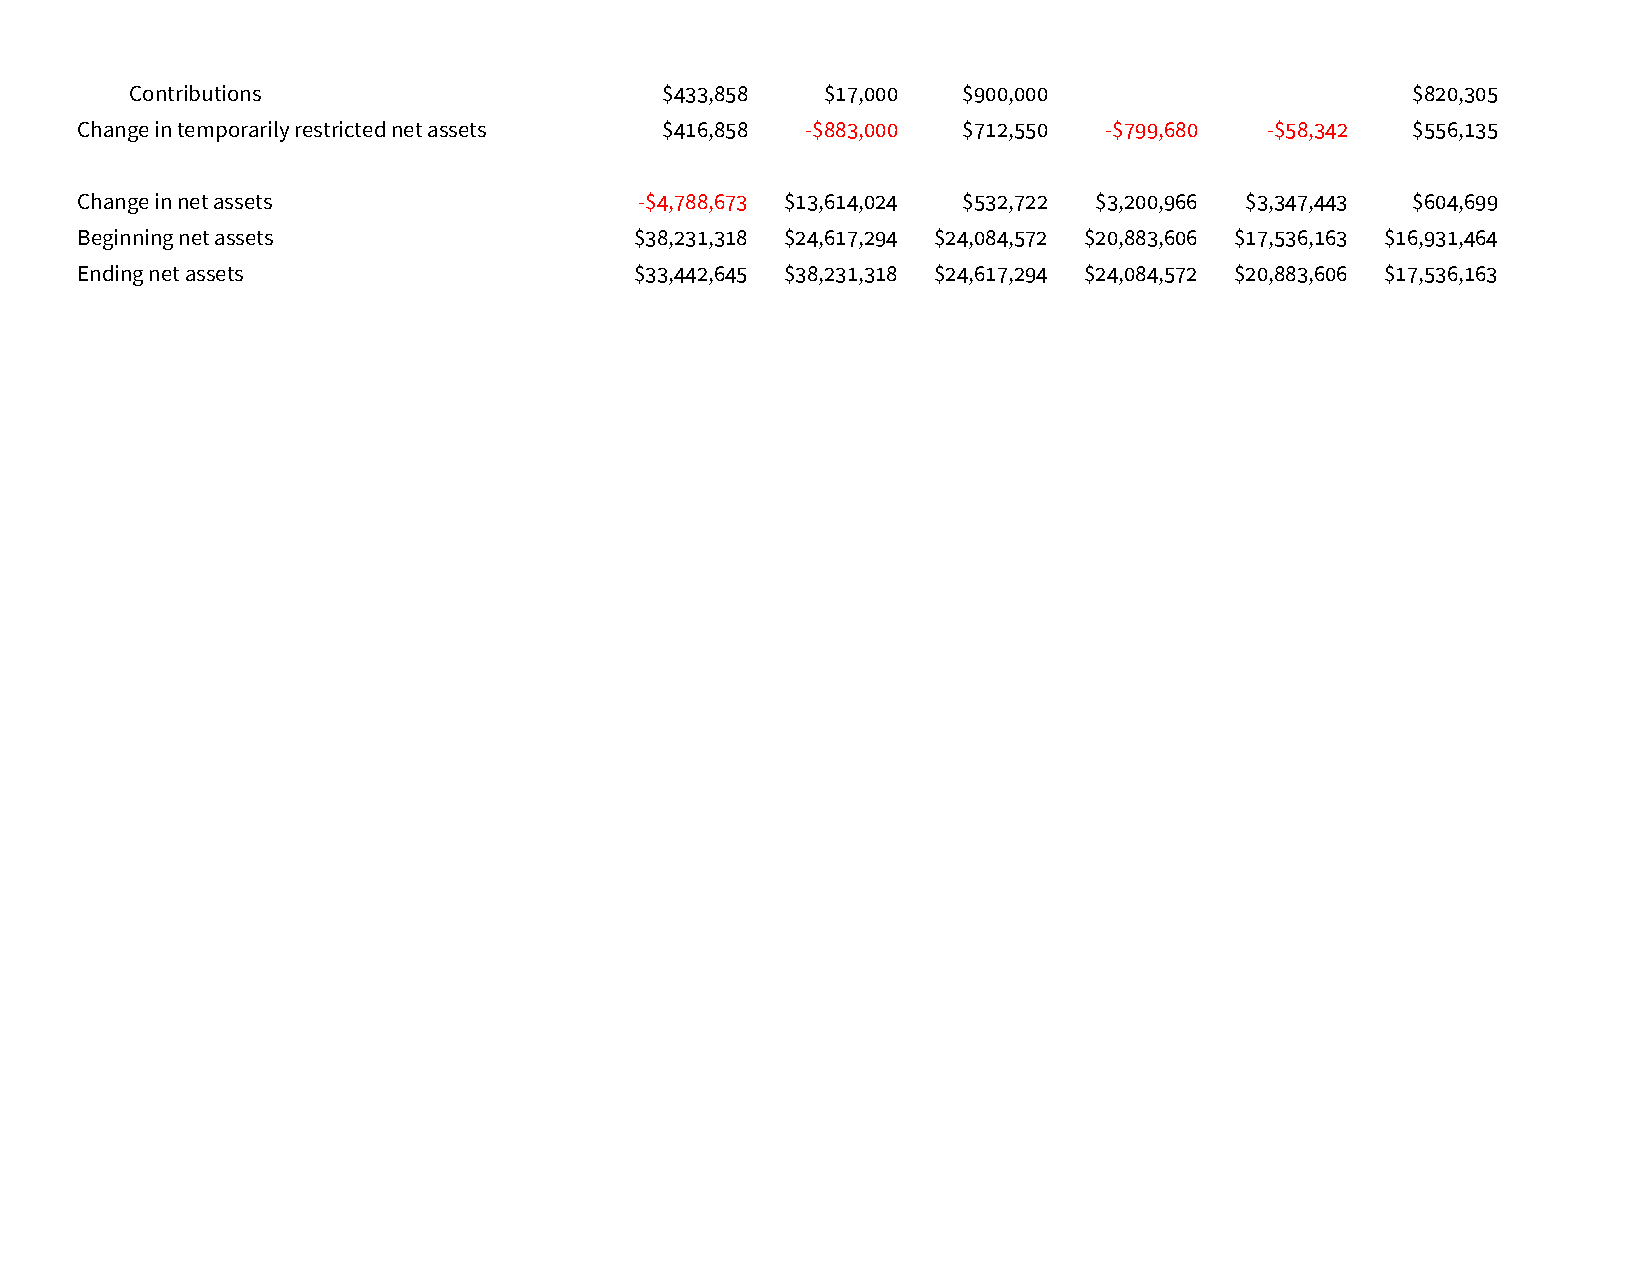
\includegraphics[width=\textwidth]{Consolidated Financial Statements/v5_Spreadsheets/Consolidated_Activities_Years_2010-2022 PDF pages/.pg_0002.pdf}\\ %chktex 8
% \end{figure}

%%% Local Variables:
%%% mode: latex
%%% TeX-master: "Rocketship_Education-An_Exploratory_Public_Policy_Case_Study"
%%% End:

\end{appendices}

%%%%%%%%%%%%%%%%%%%%%%%%%%%%%%%%%%%%%%%%%%%%%%%%%%%%%%%%%%%%%%%%% 
\backmatter{}
%%%%%%%%%%%%%%%%%%%%%%%%%%%%%%%%%%%%%%%%%%%%%%%%%%%%%%%%%%%%%%%%%
\clearforchapter{\small\printindex}
% \linenumbers%
\clearforchapter%%% Time-stamp: <2023-07-13 13:43:01 vladimir>
%%% Copyright (C) 2019-2023  Vladimir G. Ivanović
%%% Author: Vladimir G. Ivanović <vladimir@acm.org>
%%% ORCID: https://orcid.org/0000-0002-7802-7970
\chapter{Colophon}
\small\OnehalfSpacing%

Two versions of this dissertation are available. The contents of both are identical; only the formatting differs.
\begin{enumerate}[nosep]
  \item \url{https://leonora.org}\\\noindent%
  This version, the readable version, has been formatted according to standard typographic practice which emphasizes  readability, and it is hoped, good taste and elegance. 
  \item \url{https://sjsu.edu}\\\noindent%
  This version, the official, submitted version, has been formatted to meet the SJSU Ed.D. doctoral dissertation guidelines. You should read this version only under duress.
\end{enumerate}

This dissertation was created nearly entirely with free, open source programs.\footnote{Two closed source, proprietary programs were used to manipulate PDF files, themselves proprietary programs until recently. These programs could have been replaced with FOSS programs, but the results would not have been as high quality.} The typefaces, the text editor, the markup language, the reference manager, the operating system, and many utilities are all FOSS (free, open source software).
\begin{center}
  \textbf{\adforn{21}\qquad\adforn{21}\qquad\adforn{11}\qquad\adforn{49}\qquad\adforn{49}}
\end{center}
The body and headings were set in 12pt Alegreya. The Alegreya family of serif \& sans serif typefaces was designed by Juan Pablo del Peral of Huerta Tipográfica in 2011 and immediately won praise and awards. It is a classic Renaissance typeface, a kind that was first developed in the fourteenth and fifteenth centuries in northern Italy. It comes in Regular, Medium, Bold and Black weights, all of which are available in Roman and Italic styles. There is a full set of Greek and Cyrillic letters as well as Latin small caps. All have a full set of ligatures, and Old Style, and Lining numerals. Notably, all the numerals share the same width so they line up regardless of which style is being used. (Multiplication using Roman numerals, anyone?) If any criticism can be leveled against the Alegreya superfamily, it is that the family doesn't include display sizes and doesn't contain swash characters. Otherwise it is nearly perfect.
\begin{center}
  \textbf{\adforn{21}\quad\quad\adforn{21}\quad\quad\adforn{11}\quad\quad\adforn{49}\quad\quad\adforn{49}}
\end{center}
The programs \TeX{} \& \LaTeX{}  and the document class \texttt{memoir} were used to format this dissertation. \LaTeX  was created by Leslie Lamport as a user-friendly version of one of the first digital typesetting systems, \TeX . \TeX  is one of the masterpieces of computer programming whose author, Donald Knuth, won the Turing Award in 1974. It is a testament to Knuth's brilliance as both a mathematician and a programmer that \TeX  is still in use more than four decades later and arguably has no peers when it comes to typesetting complex mathematics and scientific material. It is, however, awkward to use and hard to learn. Fortunately, Leslie Lamport wrapped \TeX  in a macro system, \LaTeX , which was orders of magnitude easier to use than \TeX  itself.
LaTeX is extraordinarily flexible because there are thousands of packages which implement specialized tasks. Currently, CTAN (the Comprehensive TeX Archive Network) has just shy of 6000 packages which can be downloaded. One of those packages implements the class \texttt{memoir} that was used here. It was written by Peter Wilson, and released in 2001. (I'm listed as a contributor to \texttt{memoir}, but in truth I really only just corrected some minor typos.)
\newpage
\begin{center}
  \textbf{\adforn{21}\quad\quad\adforn{21}\quad\quad\adforn{11}\quad\quad\adforn{49}\quad\quad\adforn{49}}
\end{center}
Wilson's muse is Robert Bringhurst, author of \textit{The Elements of Typographic Style}, which some consider to be the definitive book on typography and book design. It is certainy the most elegant. The package \texttt{memoir} would undoubtedly meet with Bringhurst's approval.  The class \texttt{memoir} provides in one package nearly everything a person needs to produce ``beautiful books'' (Knuth's words). Although creating a bibliography, glossary, and an index are possible in \texttt{memoir}, specialized packages are normally used instead of the built-in ones supplied by \texttt{memoir}.
\begin{center}
  \textbf{\adforn{21}\quad\quad\adforn{21}\quad\quad\adforn{11}\quad\quad\adforn{49}\quad\quad\adforn{49}}
\end{center}
Zotero is a program to manage and maintain a bibliographic database and to provide citations on demand. It, along with the text editor GNU Emacs (``an operating system disguised as an editor'') and the package \texttt{reftex}, cooperate with \texttt{memoir} to provide a complete system for writing scholarly papers, theses, reports, and dissertation.
\begin{center}
  \textbf{\adforn{21}\quad\quad\adforn{21}\quad\quad\adforn{11}\quad\quad\adforn{49}\quad\quad\adforn{49}}
\end{center}
All of these program run on Linux, a version of Unix using a particular distribution, Arch Linux, one of many. It is notable that GNU Linux, GNU Emacs, \TeX  and \LaTeX\_ are all programs that are decades old, have never been replaced or superseded, are constantly being improved, and are actively used. They share a common set of characteristics: their fundamental architecture is sound, extensibility is a core feature, and they and thousands of specialized packages are freely available. I predict that iPhones will be the faintest of memories when GNU Unix, GNU Emacs, and \LaTeX start to fade from view.
%%% Local Variables:
%%% mode: latex
%%% TeX-master: "Rocketship_Education-An_Exploratory_Public_Policy_Case_Study"
%%% End:


\end{document}

%%% Local Variables:
%%% mode: latex
%%% TeX-master: "Rocketship_Education-An_Exploratory_Public_Policy_Case_Study"
%%% End:
